\documentclass{beamer}
\usetheme{Darmstadt}
\usecolortheme{default}
\usepackage{draftcopy}
\usepackage{graphicx}
\usepackage{amsmath}
\usepackage{enumerate}
\usepackage{verbatim}
\beamertemplatenavigationsymbolsempty


%This script was pulled from pdflatex codes

%\MyLogo{ECO364 (International Trade) Summer 2016}
%\leftheader{Using CVS in Autominder}
%\rightheader{Using CVS in Autominder\quad\textsf{\tiny[\thepage]}}
%\rightheader{\quad\textsf{\tiny[\thepage]}}
%\rightfooter{\quad\textsf{\thepage}}

% Set the default page color and style.
%\pagecolor{white}
%\vpagecolor[lightblue]{green}
%\vpagecolor{bgblue}
%
%\hpagecolor[cyan]{white}


\title{ECO364 (International Trade) Summer 2016}
\date{June 1, 2016}
\author[Scott Orr]{Scott Orr}
\institute{University of Toronto}

\AtBeginSection[]
{
	\begin{frame}
		\frametitle{Outline}
		\tableofcontents[currentsection]
	\end{frame}
}

\begin{document}
	
	\begin{frame}
		\titlepage
	\end{frame}
	
\section{Outline}
	
\begin{frame}
	\frametitle{Section Outline}
\begin{itemize}
	\item Last Section:
	\begin{itemize}
		\item Classical Trade Model:
		\begin{itemize}
			\item Perfect Competition
			\item Comparative Advantage Based Trade
		\end{itemize}
	\end{itemize}
	\item This Section:
	\begin{itemize}
		\item Trade Policy 
		\begin{itemize}
			\item When are trade restrictions welfare improving? Why?
		\end{itemize}
		\item Trade with Increasing Returns and Imperfect Competition
		\begin{itemize}
			\item``Pro-Competitive" Gains From Trade
		\end{itemize}
		\item Trade Policy With Imperfect Competition
	\end{itemize}
	\item Today:
	\begin{itemize}
		\item The Instruments of Trade Policy (KMO Ch. 9)
			\begin{itemize}
				\item Appendix to KMO Ch 10 (Optimal Tariffs)
			\end{itemize}
	\end{itemize}
\end{itemize}
\end{frame}

\begin{frame}
	\frametitle{The Instruments of Trade Policy (KMO Ch. 9)}
\begin{center}
\textbf{Outline For Today's Lecture}
\end{center}
\begin{itemize}
\item Tariffs
\begin{itemize}
\item Intro and Definitions
\item Theory: Small country
\item Theory: Large country
\end{itemize}
\item Other Instruments
\begin{itemize}
	\item Export subsidies
	\item Quotas
	\item Voluntary Export Restraints (VERs)
\end{itemize}
\end{itemize}

\end{frame}

\section{Tariffs}

\begin{frame}
	\frametitle{Tariffs: Definitions}
Broad definition: A tariff is a tax on imports. The tax can take a variety of forms:
\begin{itemize}	\vspace{3mm}
	\item 	\textbf{Specific tariff}: tax levied as a fixed charge for each unit imported
	\begin{itemize}
		\item Revenue = $(p-t)q$\\ \vspace{2mm}
	\end{itemize} 
	\item \textbf{Ad-valorem tariff}: tax levied as a fraction of the value being imported
	\begin{itemize}
		\item Revenue = $(1-\tau)pq$\\ \vspace{2mm}
	\end{itemize} 
	\item \textbf{Compound duty}: mixture of specific and ad-valorem tariff
	\begin{itemize}
		\item Revenue = $(1-\tau)(p-t)q$\\ \vspace{2mm}
	\end{itemize} 
\end{itemize}
	
\end{frame}

\subsection{Definitions and Introduction}

\begin{frame}
\frametitle{Tariffs in practice}

Tariffs have generally fallen over the last 20 years
\begin{itemize}
  \item Canada: Average Tariff Rates 
	  \begin{itemize}
	  	\item 1996: 7.82 \%
	  	\item 2014: 1.43 \%
	  \end{itemize}
	   \item United States: Average Tariff Rates 
	    \begin{itemize}
	    	\item 1996: 4.44 \%
	    	\item 2014:  2.74 \%
	    \end{itemize}
	   \item China: Average Tariff Rates 
	   \begin{itemize}
	   	\item 1994: 33.32 \%
	   	\item 2014: 7.74 \%
	   \end{itemize}
\end{itemize}

\begin{center}
	Source: World Bank WITS database. All tariff rates are simple averages.
\end{center}

\end{frame}



\begin{frame}
	\frametitle{Tariffs in practice}
Tariff rates vary widely by product group
\begin{itemize}
  \item Canada: Average Tariff Rates in 2014 by Product Groups
  \begin{itemize}
	\item Animals : 10.70 \%
	\item Textiles and Clothing: 8.77 \%
	\item Food Products: 8.03 \%
	\item Footwear: 7.33 \%
	\item Chemicals 1.09 \%
	\item Fuels: 0.62 \%
	\item Capital Goods: 0.35 \%
	\item Minerals: 0.02 \%

  \end{itemize}
\end{itemize}
\begin{center}
	Source: World Bank WITS database. All tariff rates are simple averages.
\end{center}
	
\end{frame}

\begin{frame}
	\frametitle{Tariffs in practice}
	
\begin{itemize}
		\item Why do countries use tariffs?
		\item Why are many countries actively trying to cut tariffs?
			\begin{itemize}
				\item  \textbf{Trans-Pacific Partnership (TPP)}: Recently signed trade agreement between Australia, Brunei, Canada, Chile, Japan, Malaysia, Mexico, New Zealand, Peru, Singapore, the United States, and Vietnam.
					\begin{itemize}
						\item Deal would reduce approximately 18,000 tariffs! (``Small Businesses With a Big Stake in the Pacific Trade Deal" \emph{Wall Street Journal})
					\end{itemize}
			\end{itemize}
		\item Is it beneficial for tariffs to fall?
			\begin{itemize}
				\item Most trade agreements, TPP included, are met with protest.
				\item In general, there are \emph{winners and losers} following trade agreements.
			\end{itemize}
		
	\end{itemize}
\end{frame}


\begin{frame}
	\frametitle{Theory: Tariffs in partial equilibrium}
	\begin{itemize}
		\item Up until now we have been considering a \emph{general equilibrium} model of the economy.
			\begin{itemize}
				\item General Equilibrium: Multiple markets, equilibrium price vector chosen to clear all markets.
			\end{itemize}
		\item We will now consider a \emph{partial equilibrium} model of a single market.
			\begin{itemize}
				\item Standard supply and demand framework (One good, one price per market)
				\item We will assume the existence of supply and demand curves without explicitly deriving them from consumer preferences.
			\end{itemize}
		
	\end{itemize}
\end{frame}

\begin{frame}
	\frametitle{Costs and benefits of partial equilibrium analysis}

\begin{itemize}
		\item Benefits of partial equilibrium 
		\begin{itemize}
			\item Simplifies analysis a great deal.
			\item We will be able to solve for the optimal tariff in closed form!
			\item Much of the intuition carries over to the general equilibrium case.
		\end{itemize}
		\item Costs
		\begin{itemize}
			\item We will have to ignore some secondary effects of the a tariff
				\begin{itemize}
					\item Impact on the price of Home country's export good.
					\item Income Effects
				\end{itemize}
		\end{itemize}
	\item See extra reading (Bagwell and Staiger 2010) for analysis of tariffs in general equilibrium.
		\begin{itemize}
			\item Bit advanced for this course, but a good introduction for students who want to learn a bit more.
			\item Focus on terms of trade incentives to unilaterally introduce trade barriers.
		\end{itemize}
\end{itemize}
\end{frame}

\begin{frame}
	\frametitle{Supply and Demand in a Single Industry and Single Country}
	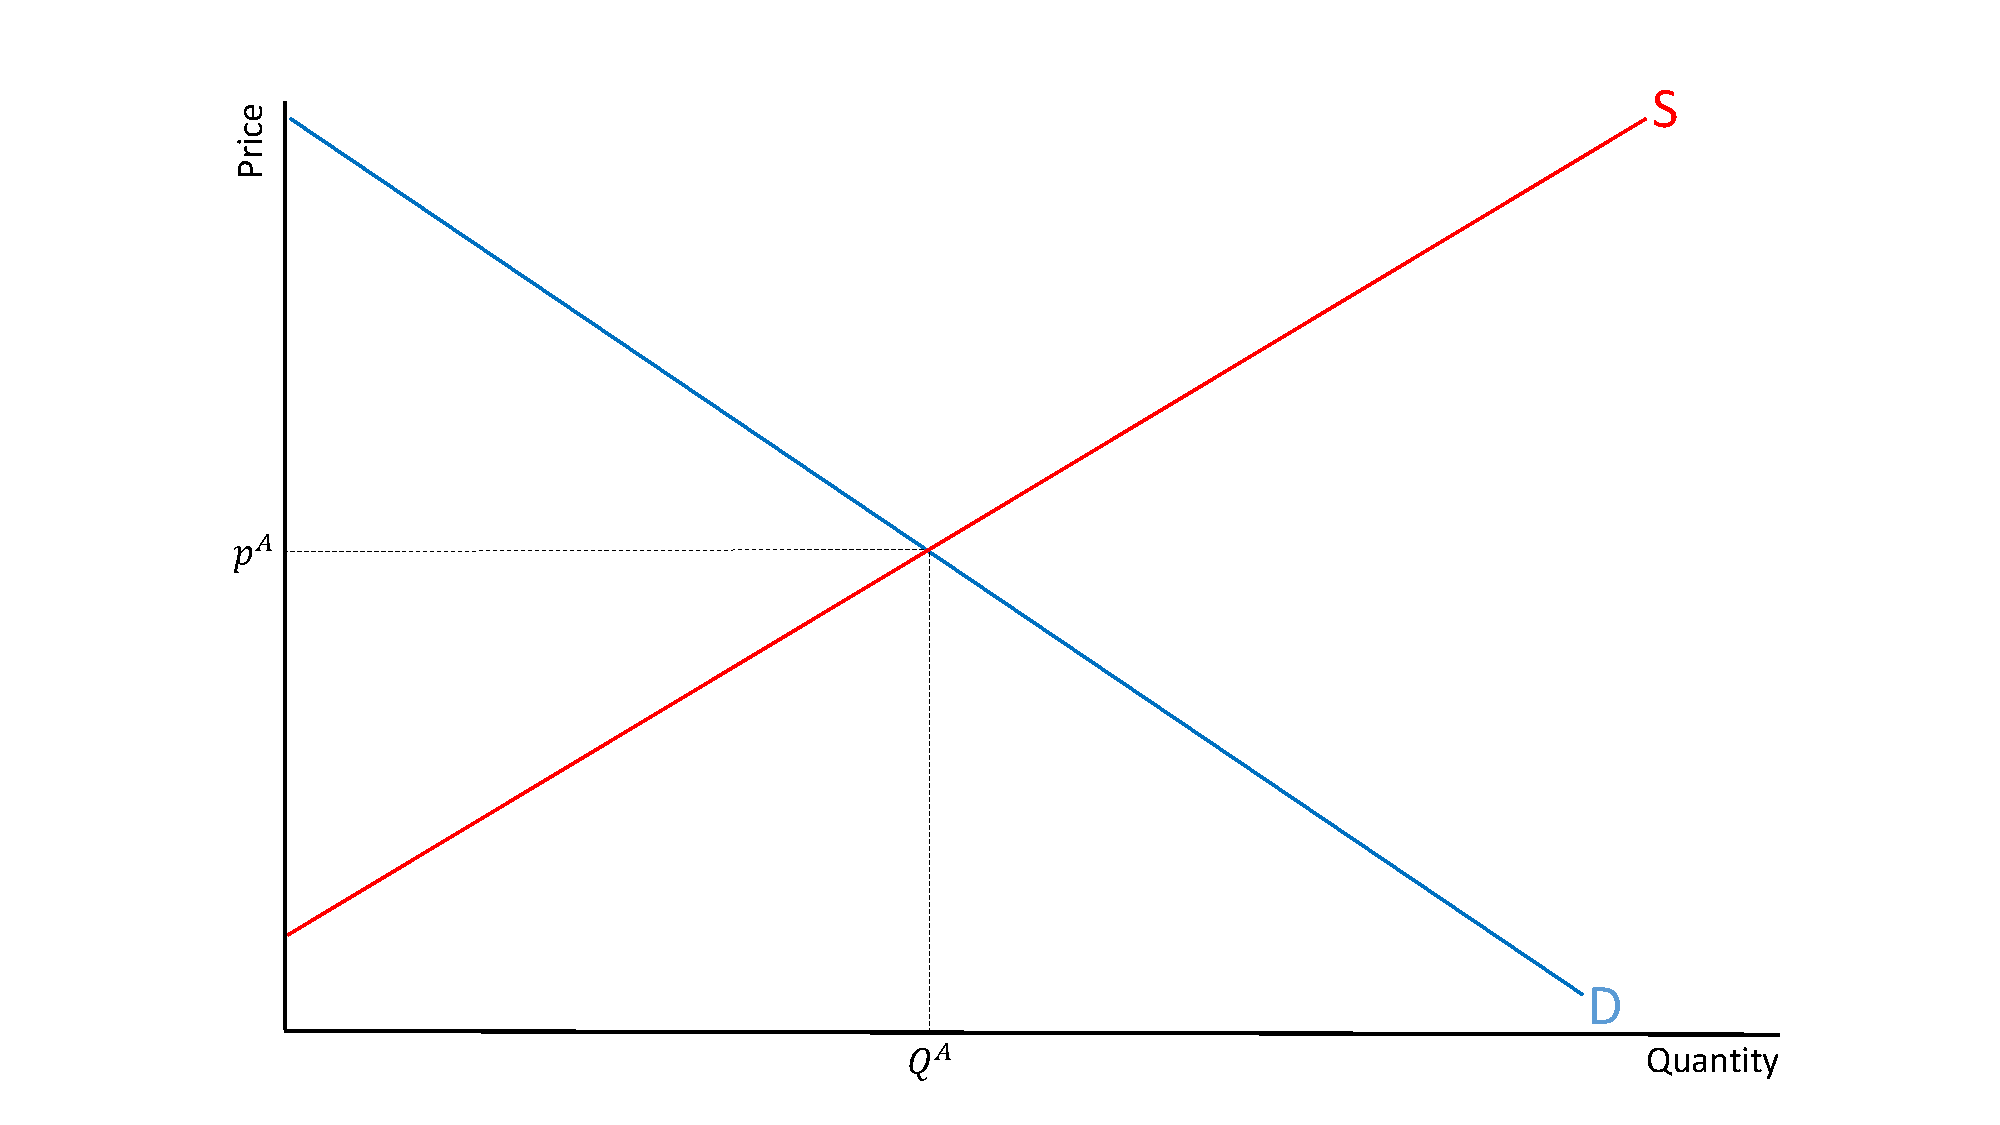
\includegraphics[scale=0.30]{SL_1.pdf} 
	\begin{itemize}
		\item Equilibrium corresponds to the \emph{autarky} price and quantity.
	\end{itemize}
\end{frame}

\begin{frame}
	\frametitle{Welfare In Partial Equilibrium: Consumers Surplus}
	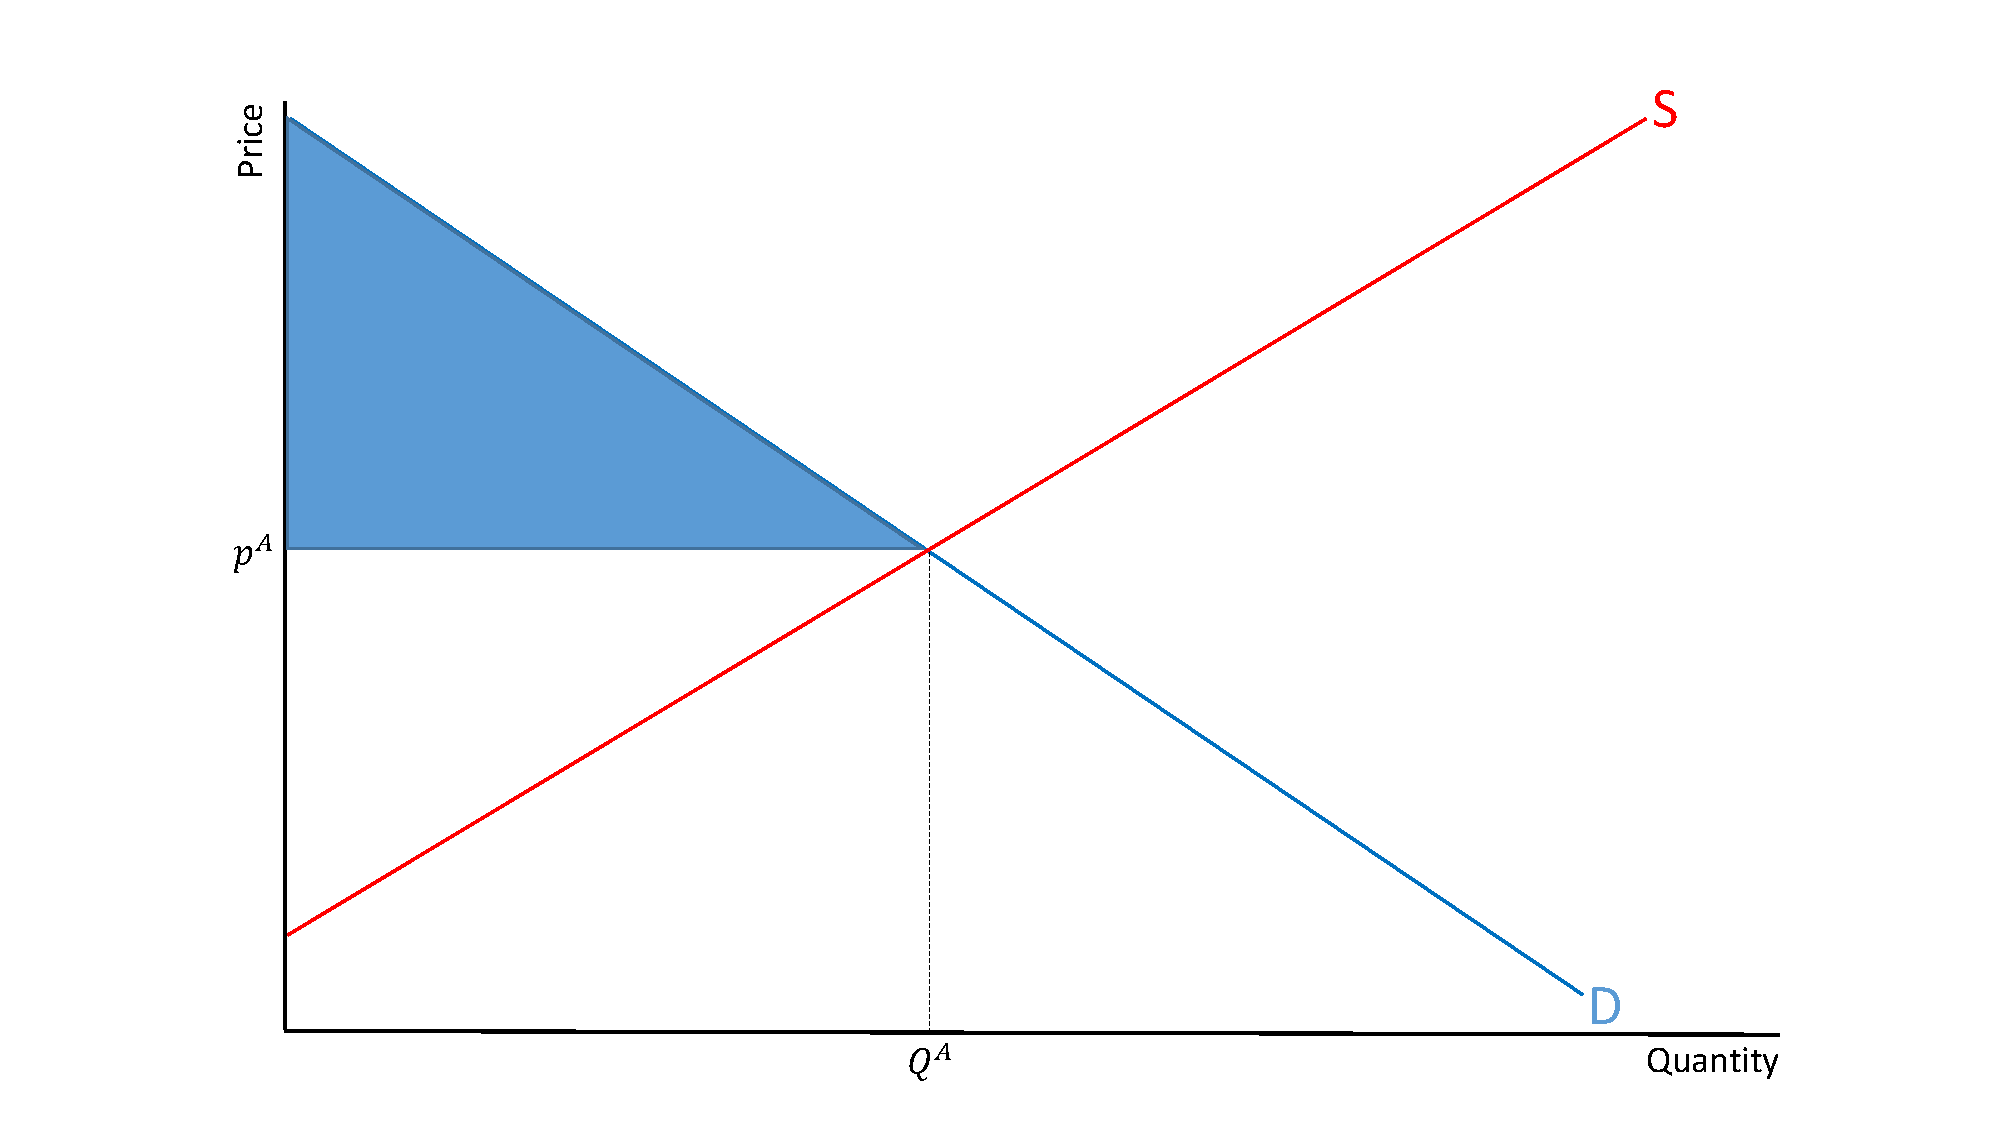
\includegraphics[scale=0.30]{SL_2.pdf}

\footnotesize
Consumer Surplus: Area under demand curve but above equilibrium price.
	\footnotesize
		\begin{itemize}
			\item Difference between willingness to pay for each marginal unit, versus what they actually pay.
		\end{itemize}

\end{frame}

\begin{frame}
	\frametitle{Welfare In Partial Equilibrium: Producer Surplus}
	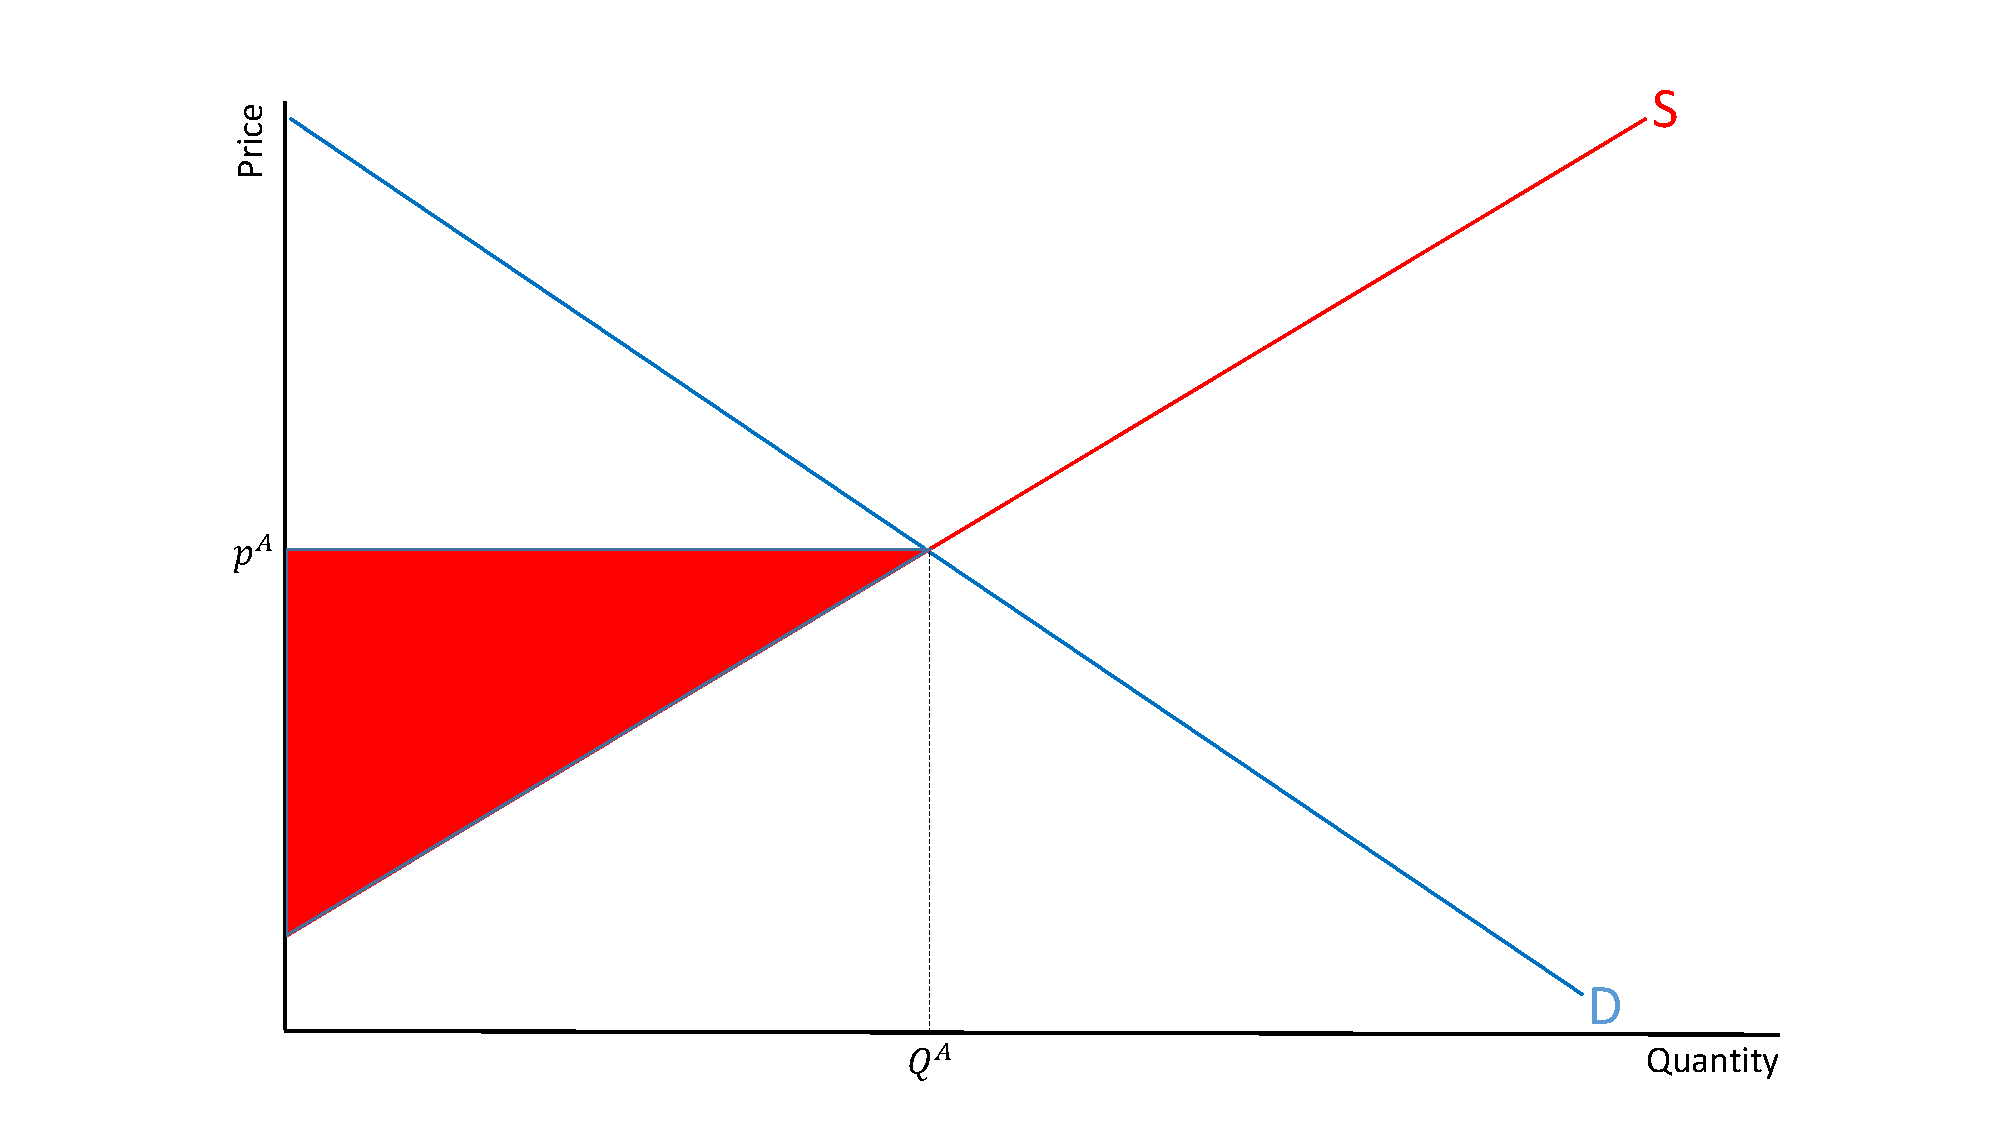
\includegraphics[scale=0.30]{SL_3.pdf}
\scriptsize
	\begin{itemize}
		\item Producer Surplus: Area above supply curve but above equilibrium price.
		\begin{itemize}
			\scriptsize
			\item Recall that supply curve is the marginal cost curve with perfect competition.
			\item Measures difference between the price earned per unit, versus the marginal cost for that particular unit.
		\end{itemize}
	\end{itemize}
\end{frame}

\begin{frame}
	\frametitle{Welfare In Partial Equilibrium: Total Surplus}
		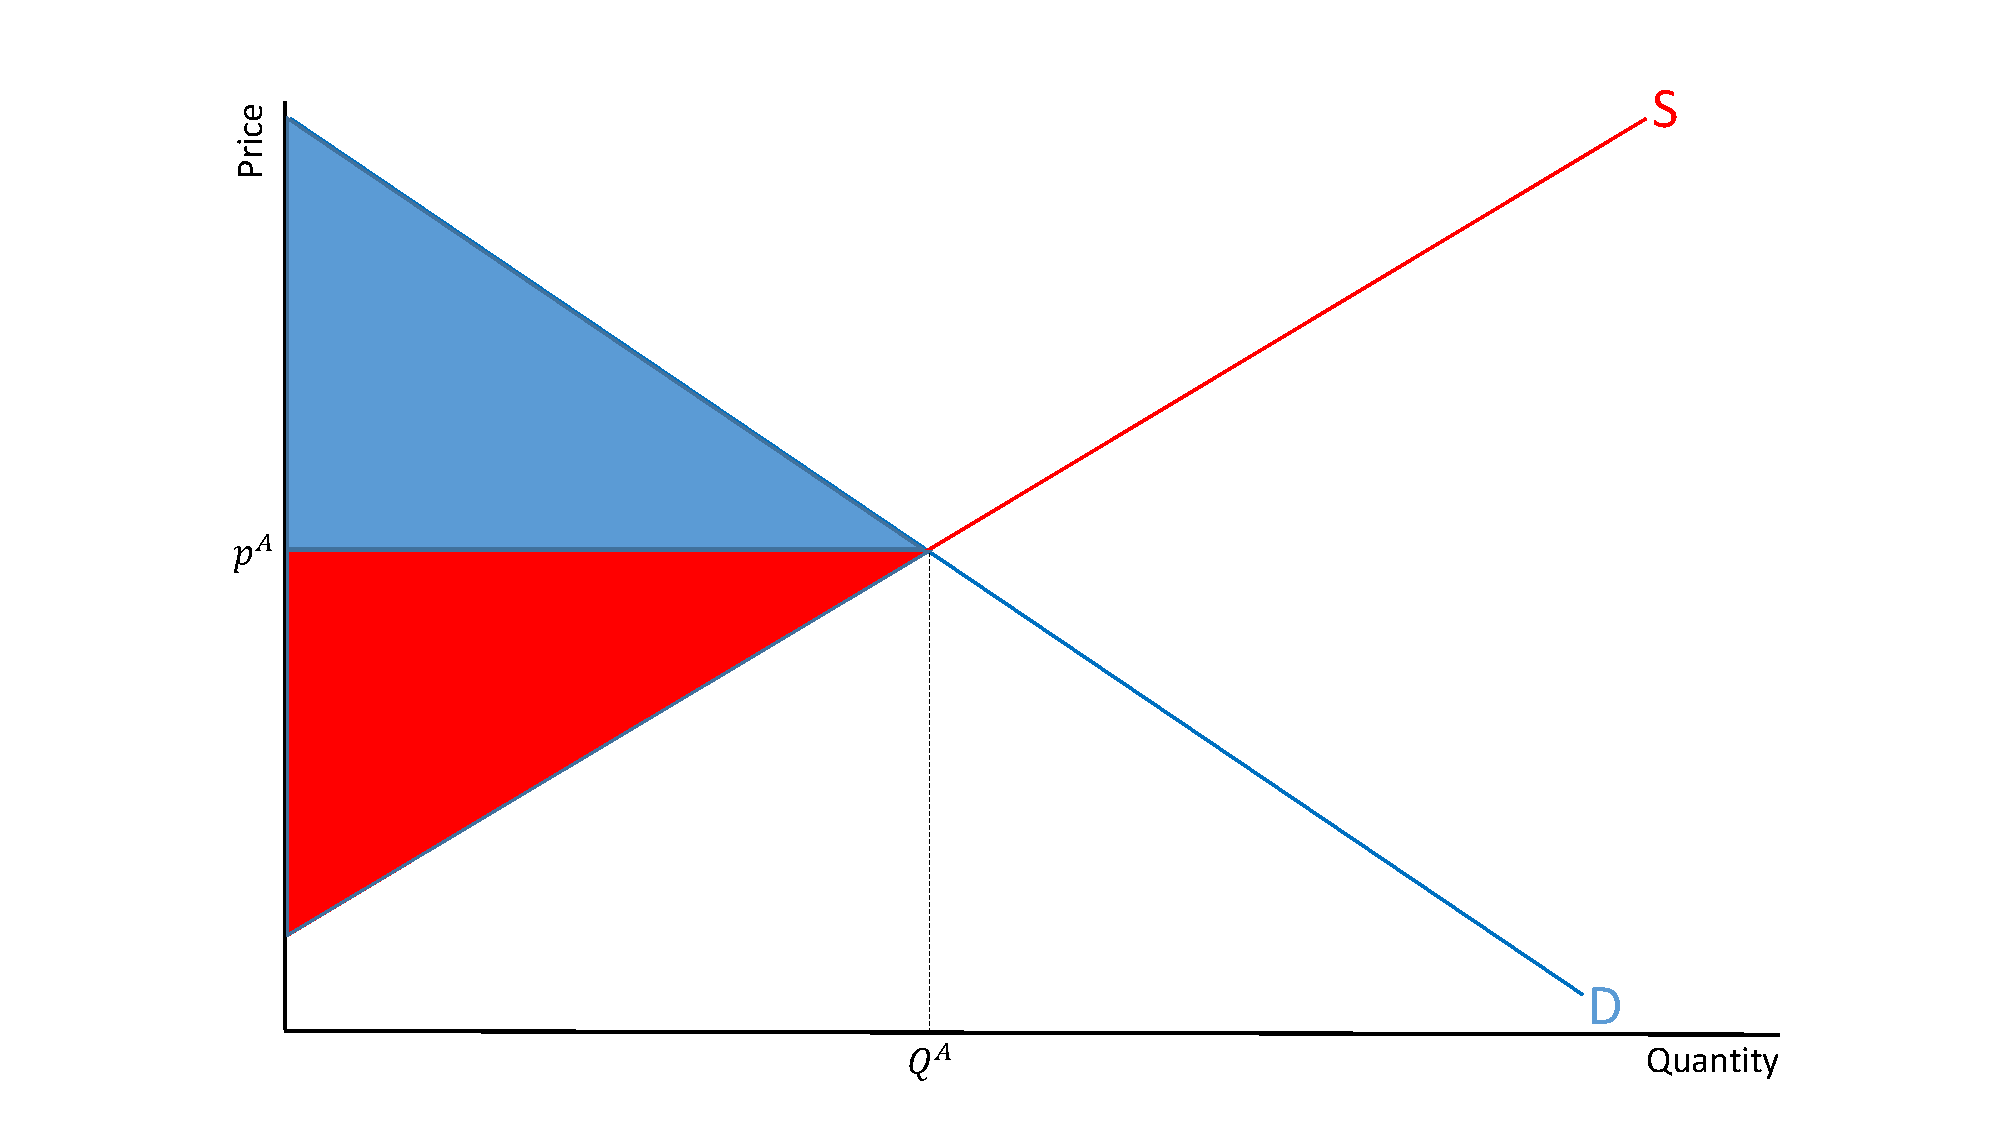
\includegraphics[scale=0.30]{SL_4.pdf}
	\begin{itemize}
		\item Total Surplus: Add up consumer and producer surplus
		\begin{itemize}
			\item Issue: Ignores distributional issues.
		\end{itemize}
	\end{itemize}
\end{frame}

\subsection{Theory: Small country}

\begin{frame}
	\frametitle{Demand and Supply: Small Open Economy}
	\begin{itemize}
		\item  Small Open Economy
			\begin{itemize}
				\item Takes world prices as given (exogenous).
				\item Price does not have to clear Home market!
			\end{itemize}
		\item Consider a single small open economy called ``Home." 
			\begin{itemize} 
				\item Assume that world prices such that Home imports the good.
					\begin{itemize}
						\item Clearly will only be the case if $p^*_W<p^A_H$
					\end{itemize}
			\end{itemize}
	\end{itemize}
\end{frame}

\begin{frame}
	\frametitle{Supply, Demand, and Imports}
	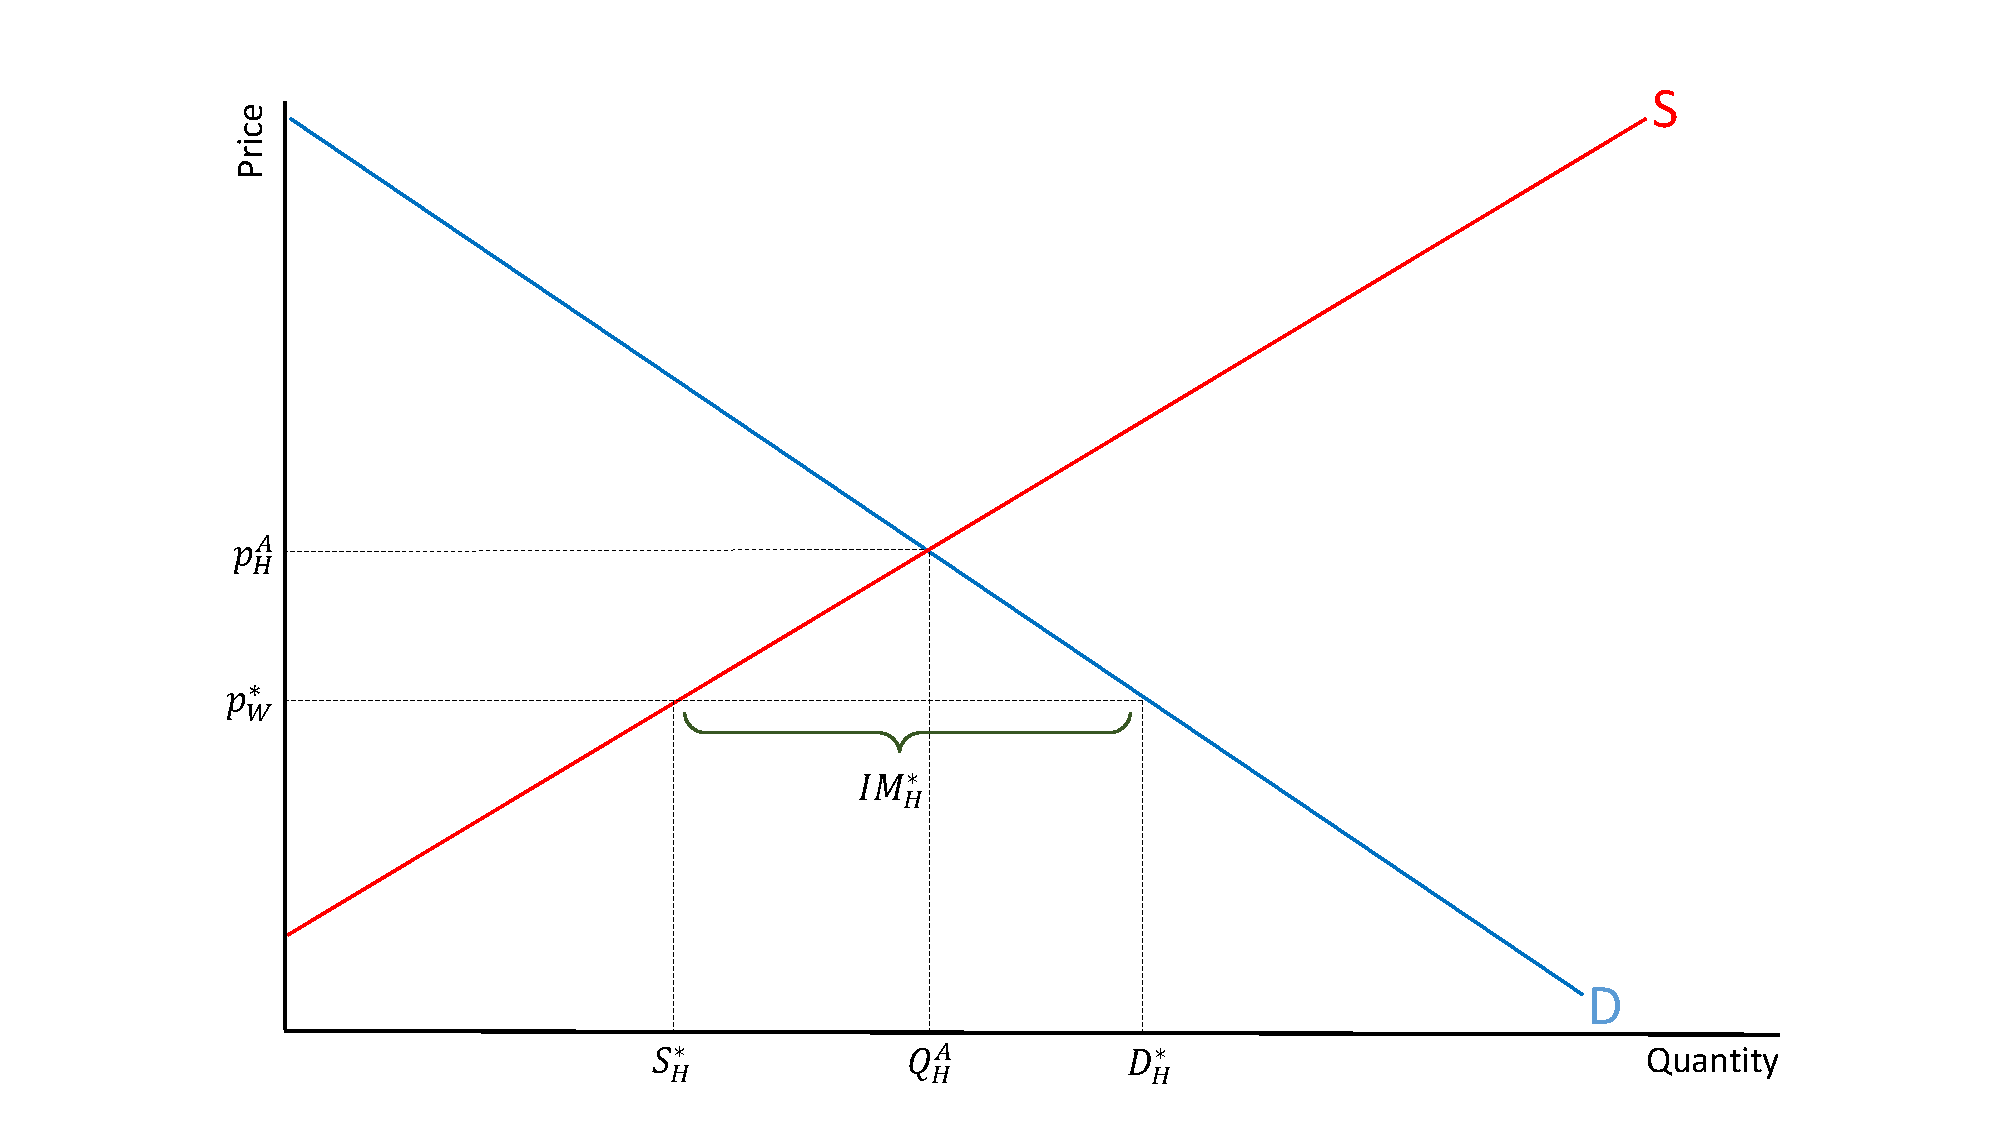
\includegraphics[scale=0.3]{SL_extra1.pdf}
\end{frame}

\begin{frame}
\frametitle{Import Demand}
	\begin{itemize}
		\item Note that imports will increase as the world price falls.
		\item Take distance between demand and supply for each world price to obtain import demand curve.
		\end{itemize}
\begin{equation}
IM(p_W)=D(p_W)-S(p_W) \nonumber
\end{equation}
	
\end{frame}


\begin{frame}
	\frametitle{Supply, Demand, and Import Demand}
	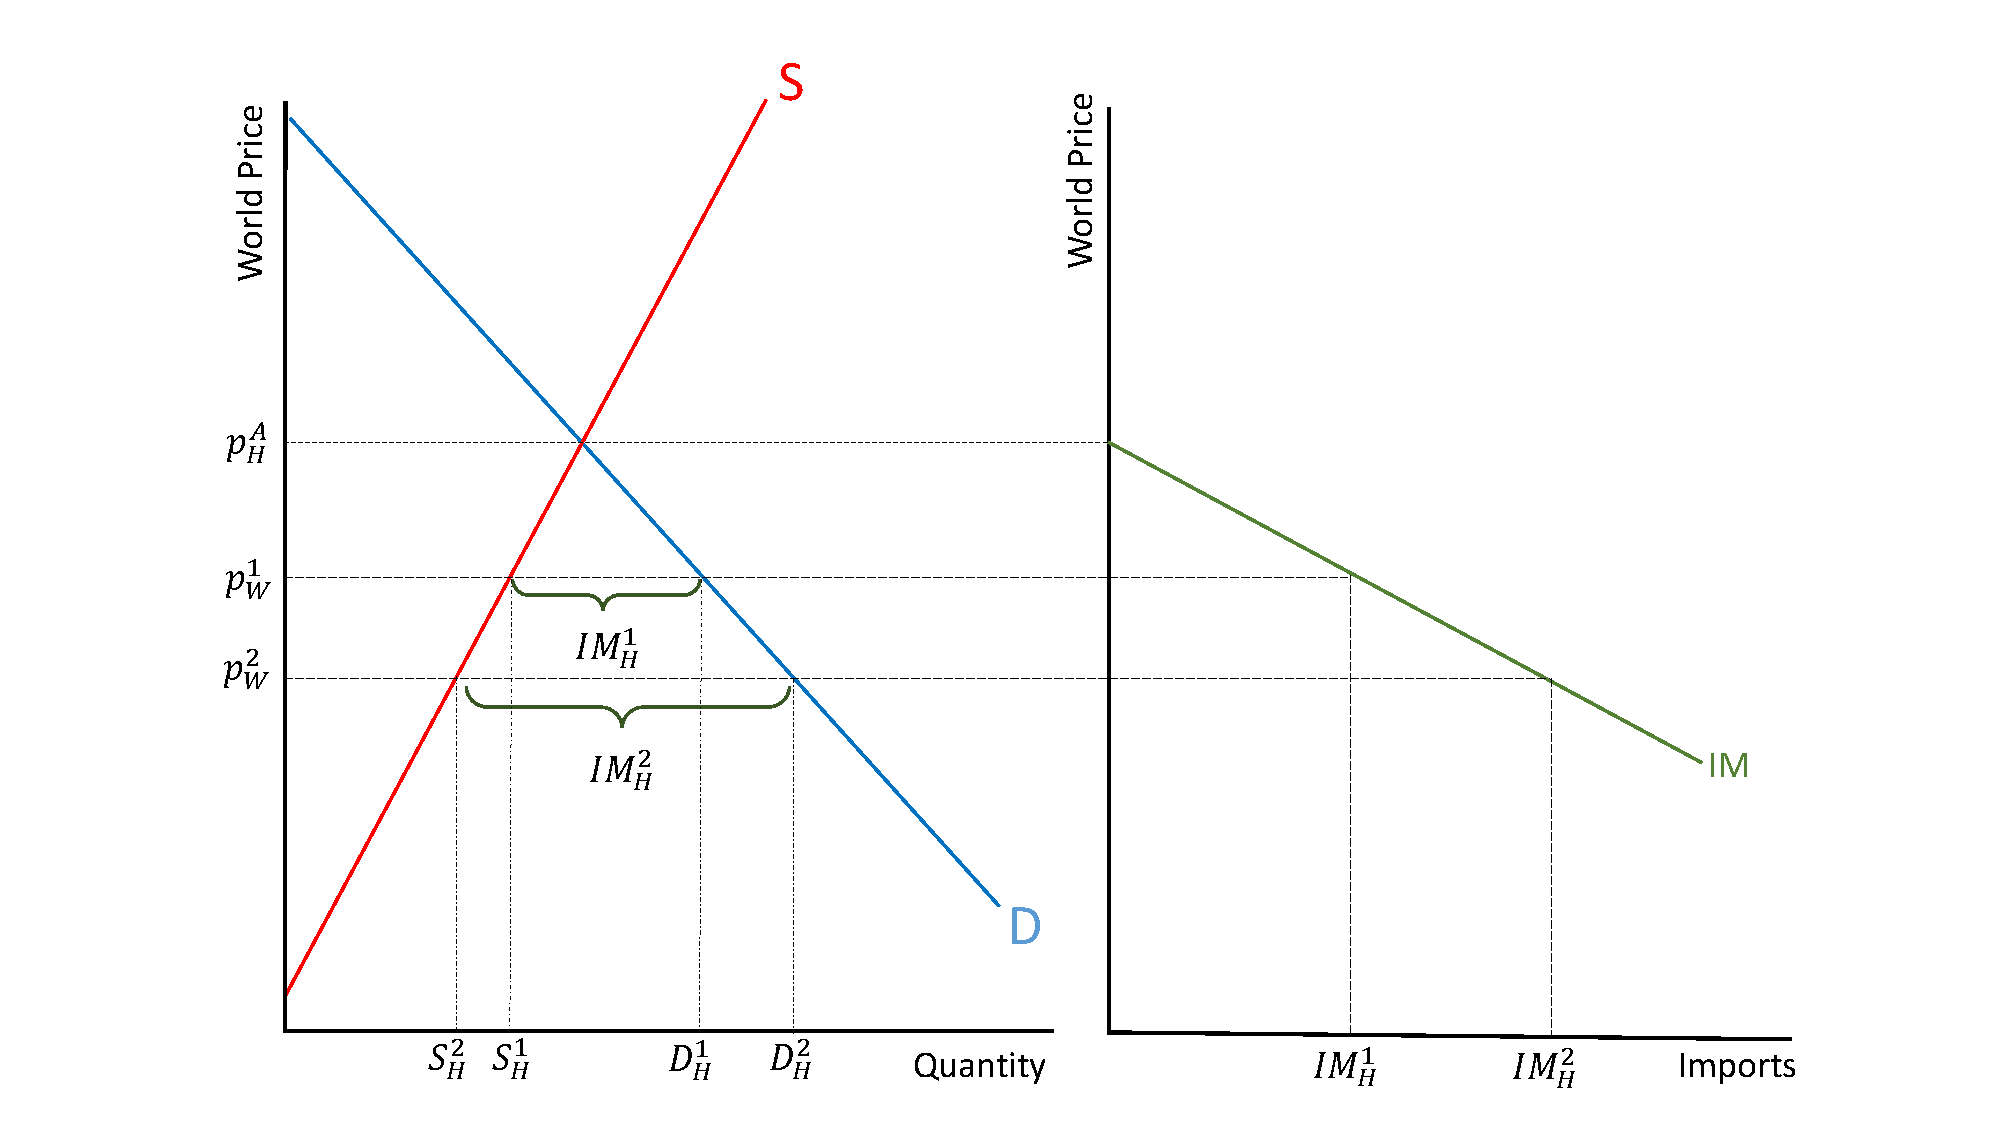
\includegraphics[scale=0.3]{SL_5.pdf}
\end{frame}

\begin{frame}
	\frametitle{Impact of Tariffs for Small Open Economy}
	\begin{itemize}
		\item For simplicity, we just consider specific tariffs, $t$.
		\item Specific tariff generates a wedge between the equilibrium world price $p_W$, and the Home price $p_H$
			\begin{itemize}
				\item Suppliers on the world market only willing to ship to this market if they receive enough to compensate them for the tariff.
					\begin{itemize}
						\item $p_H-t \geq p_W$
					\end{itemize}
				\item Home price cannot be too low, other all world suppliers would ship to the Home market!
				\begin{itemize}
					\item $p_H-t \leq p_W$
				\end{itemize}
				\item Must be that in equilibrium: $p_H-t = p_W \rightarrow p_H = p_W + t$ 
			\end{itemize}
	\end{itemize}
	\begin{center}
		\item Can show that this leads to a fall in imports, as well as welfare.
	\end{center}
\end{frame}

\begin{frame}
	\frametitle{Tariffs for Small Open Economy: Prices and Imports}
	
	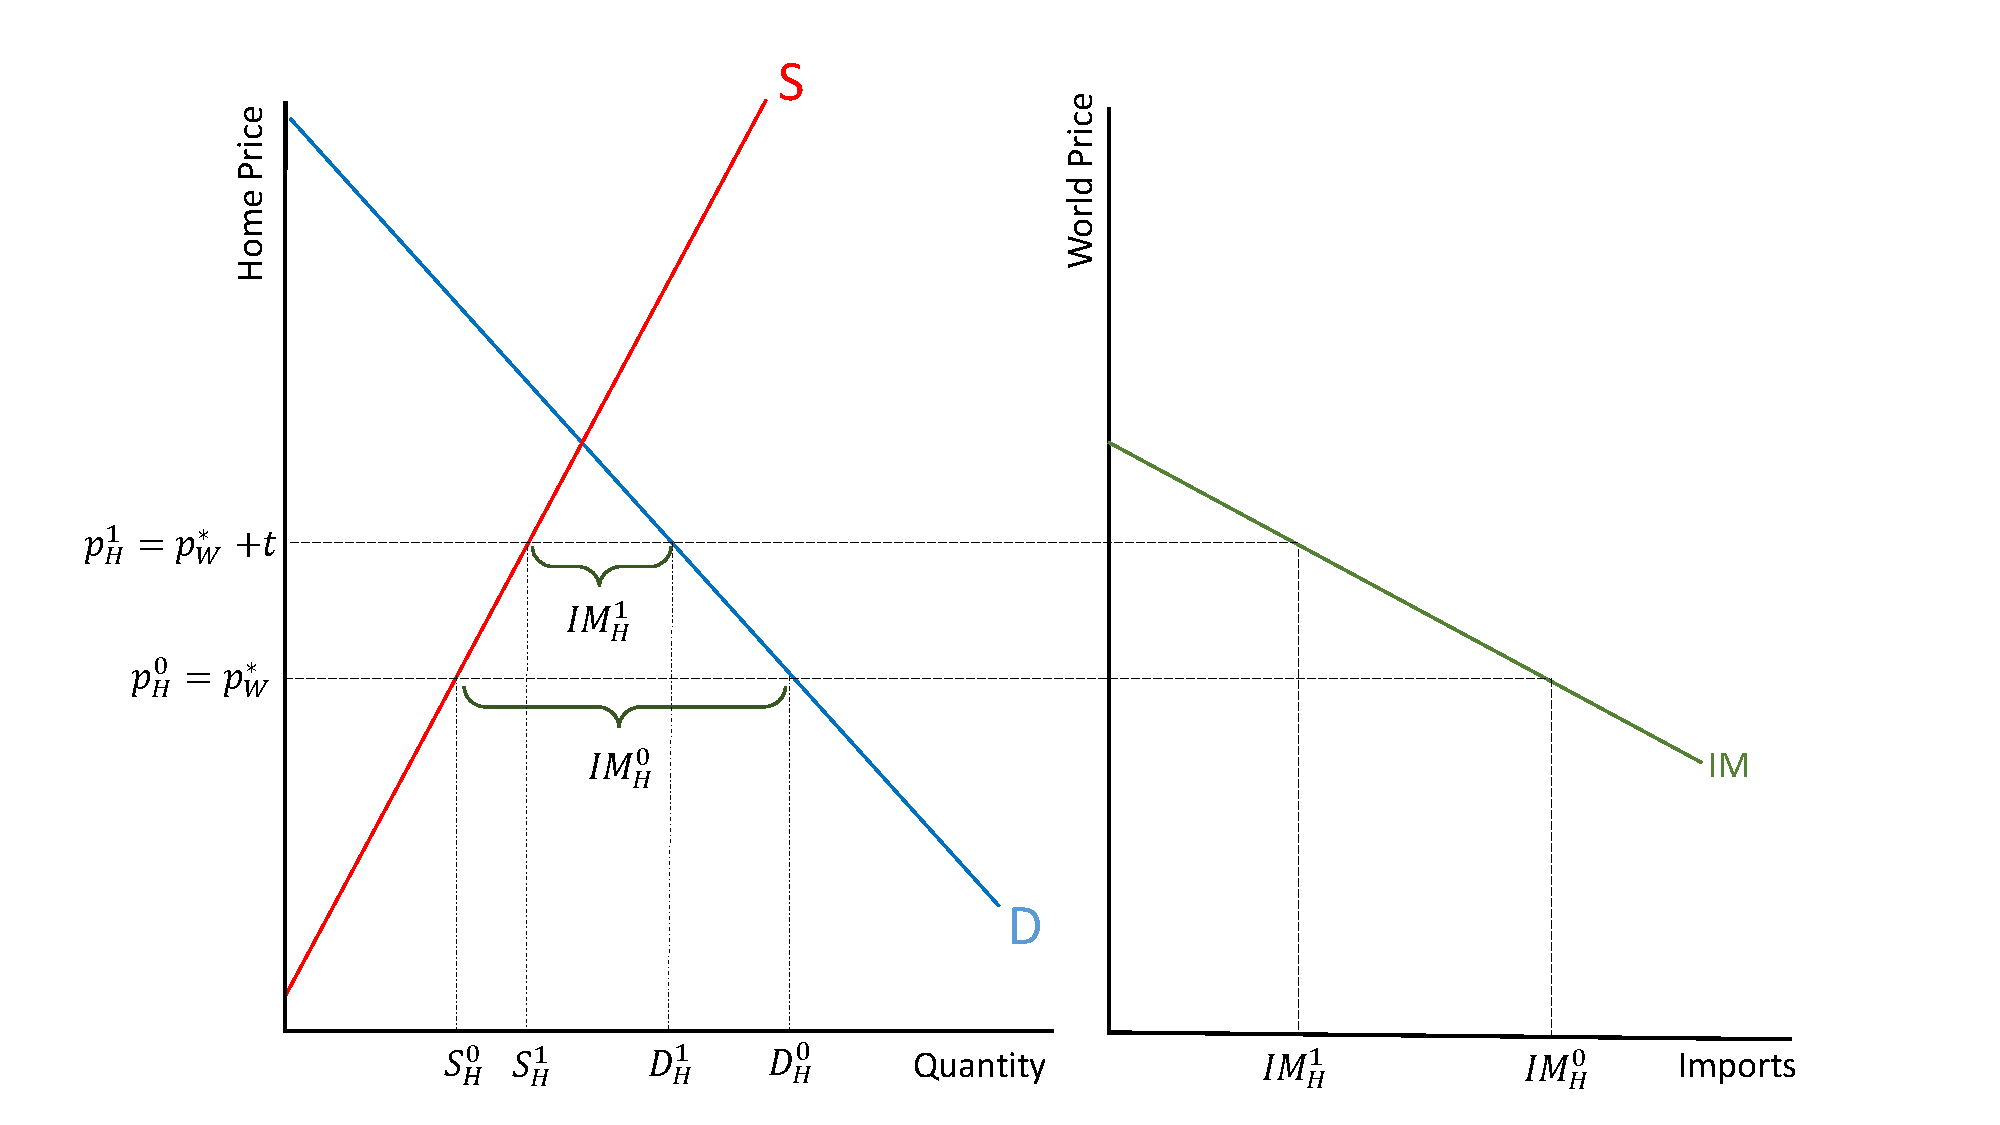
\includegraphics[scale=0.3]{SL_6.pdf}
	
\end{frame}

\begin{frame}
	\frametitle{Tariffs for Small Open Economy: Pre-Tarif Surplus}
	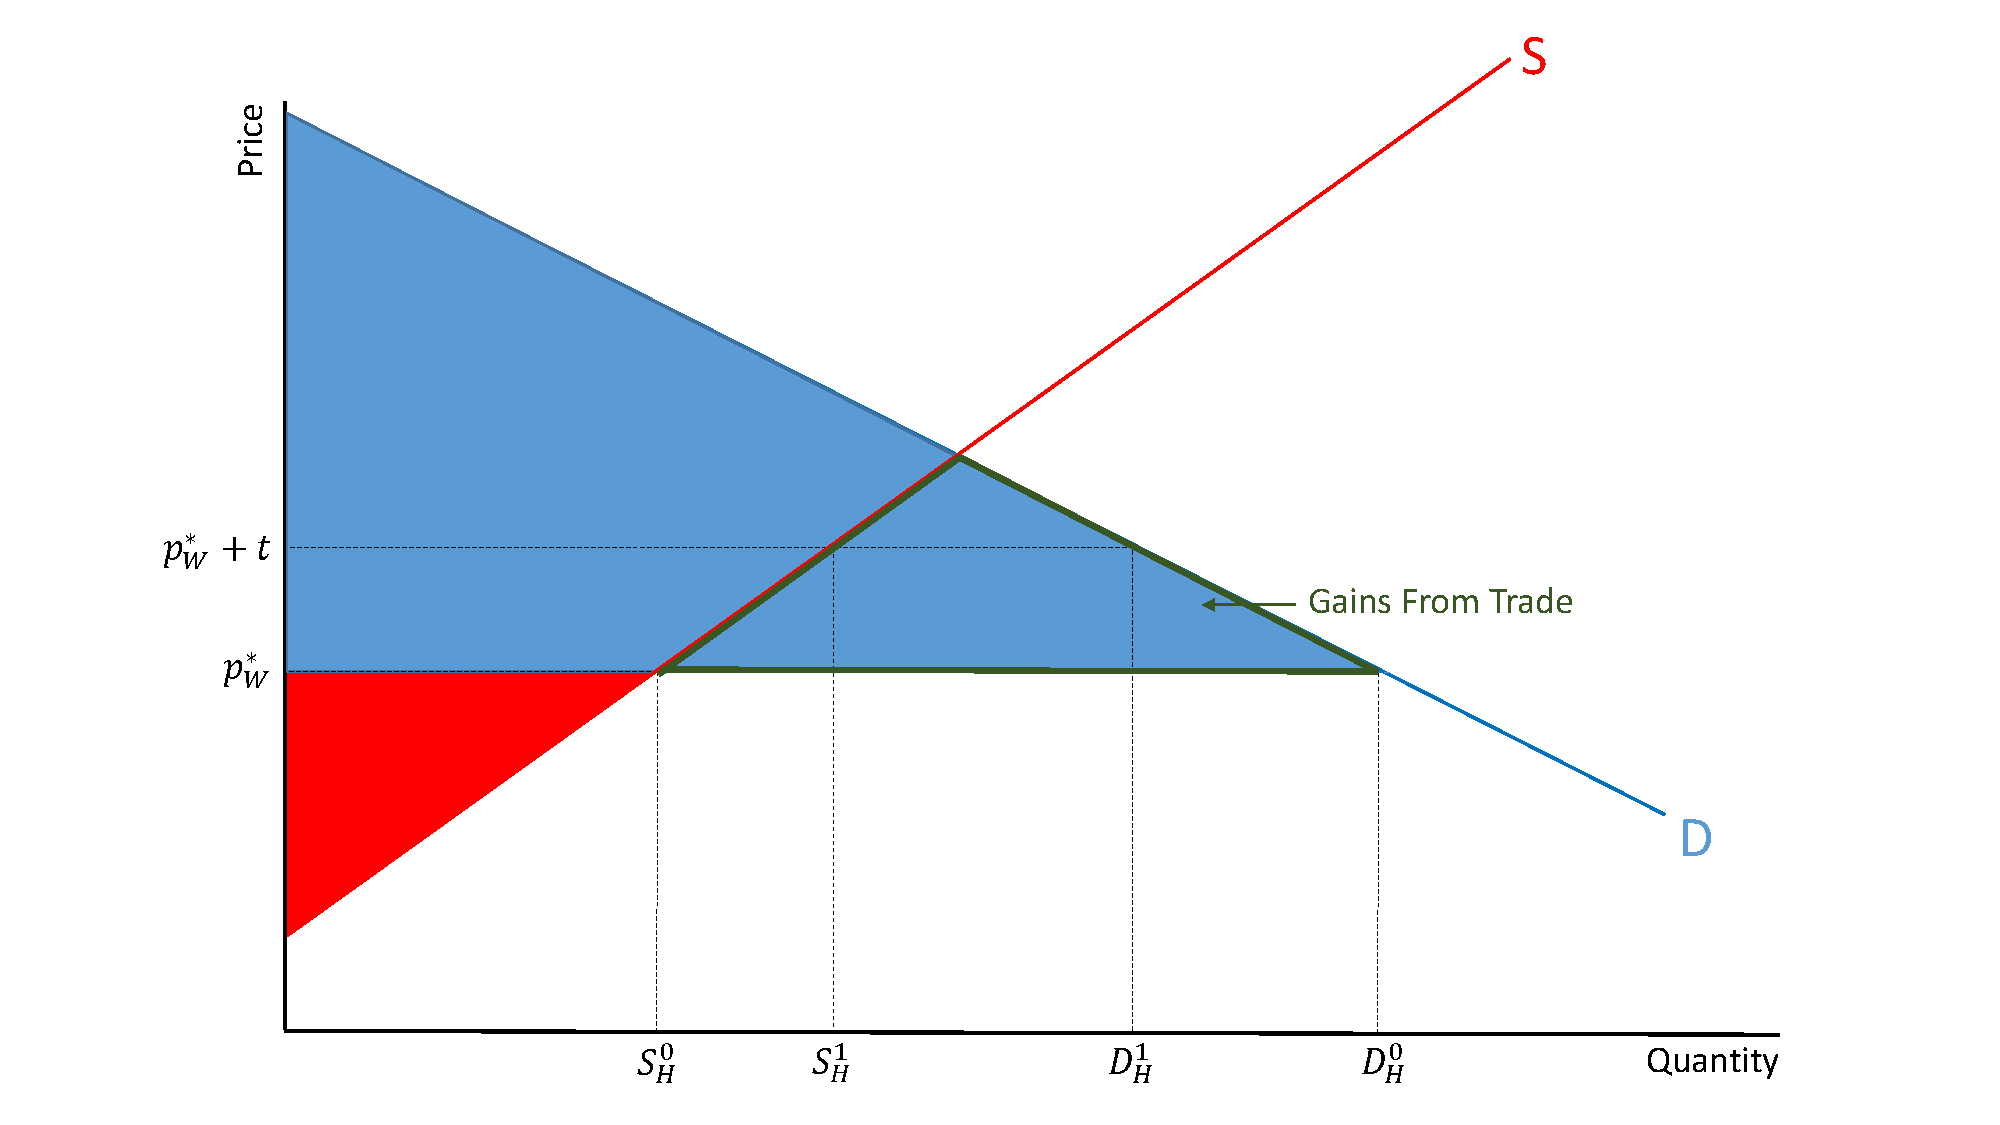
\includegraphics[scale=0.3]{SL_7.pdf}
\end{frame}

\begin{frame}
	\frametitle{Tariffs for Small Open Economy: Post-Tarif Surplus}
	
	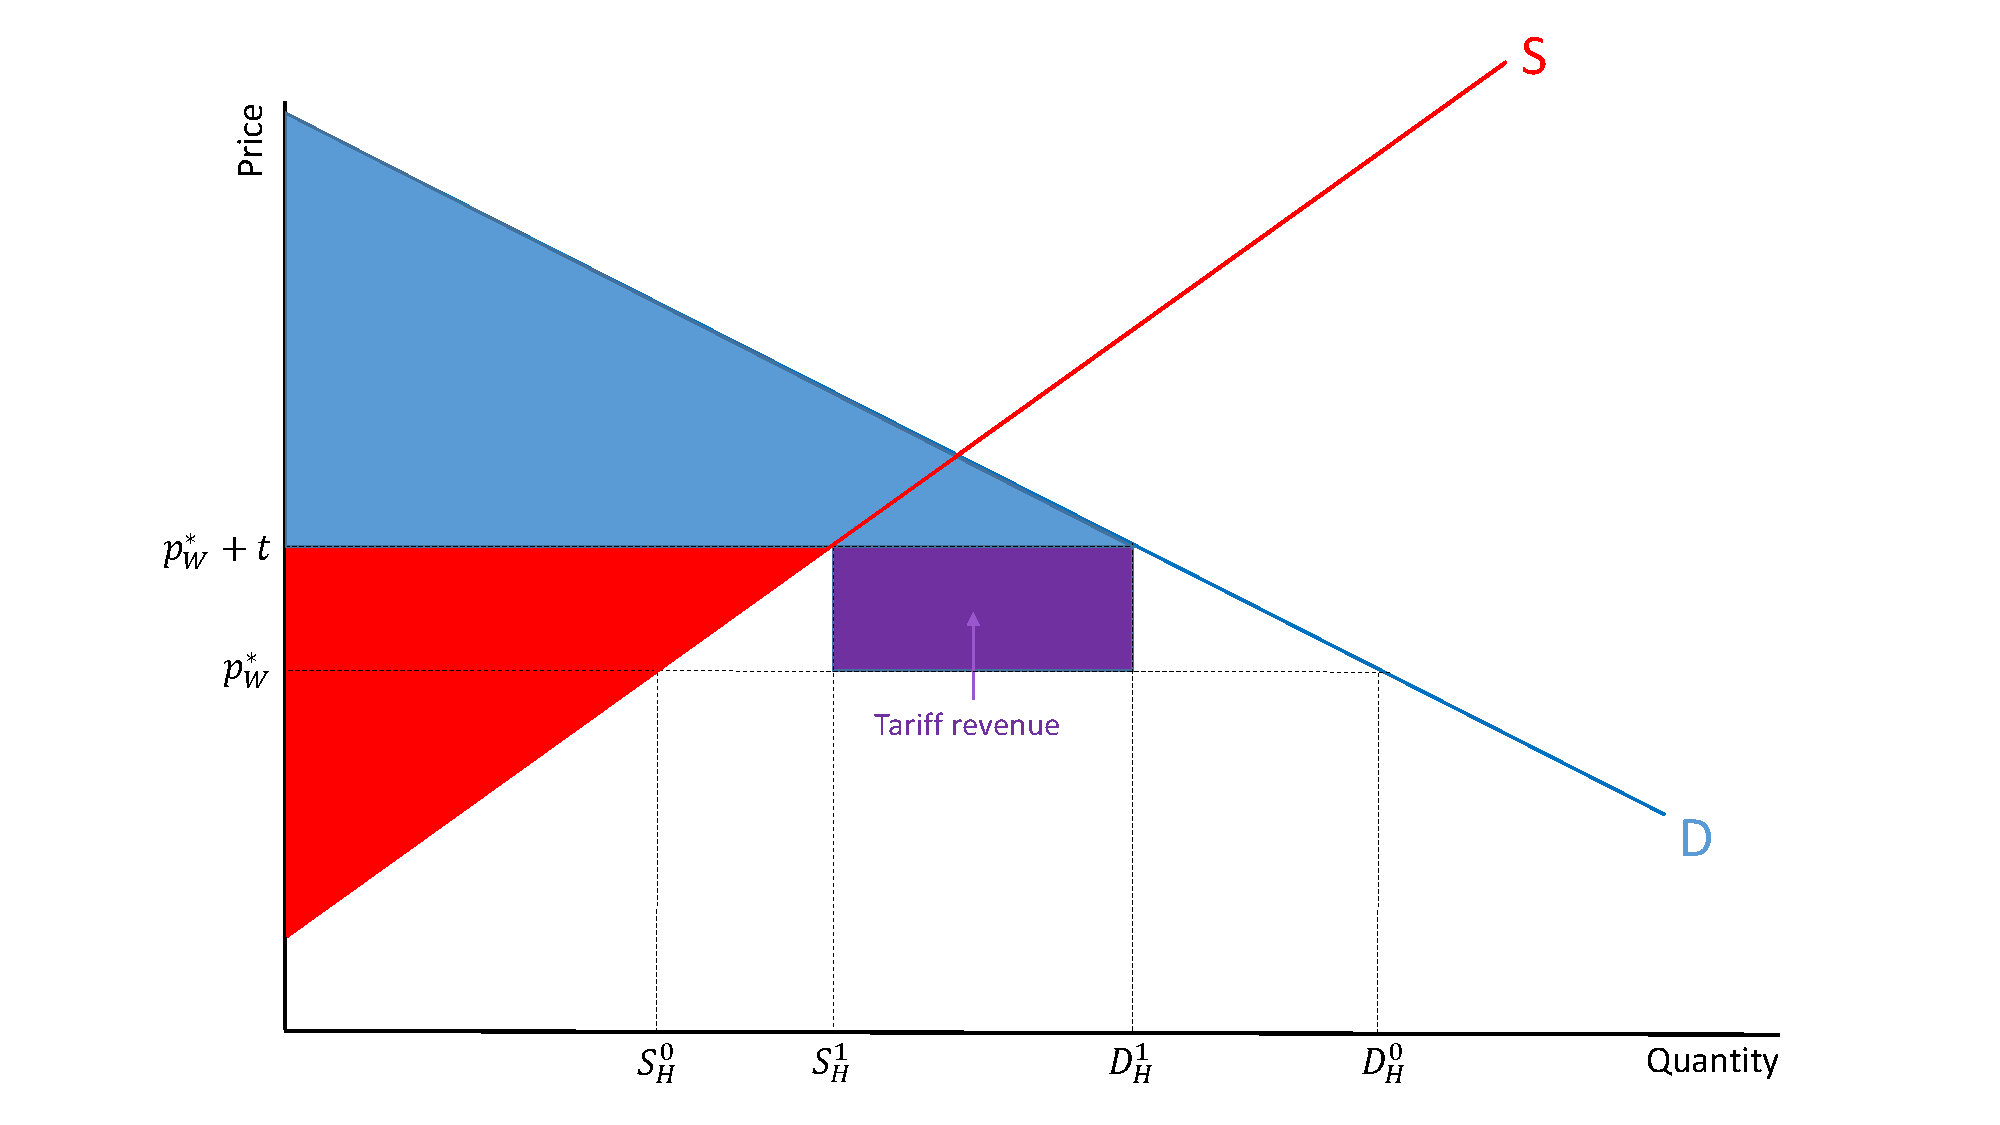
\includegraphics[scale=0.3]{SL_8.pdf}
	
\end{frame}

\begin{frame}
	\frametitle{Tariffs for Small Open Economy: Fall in Surplus}
	
		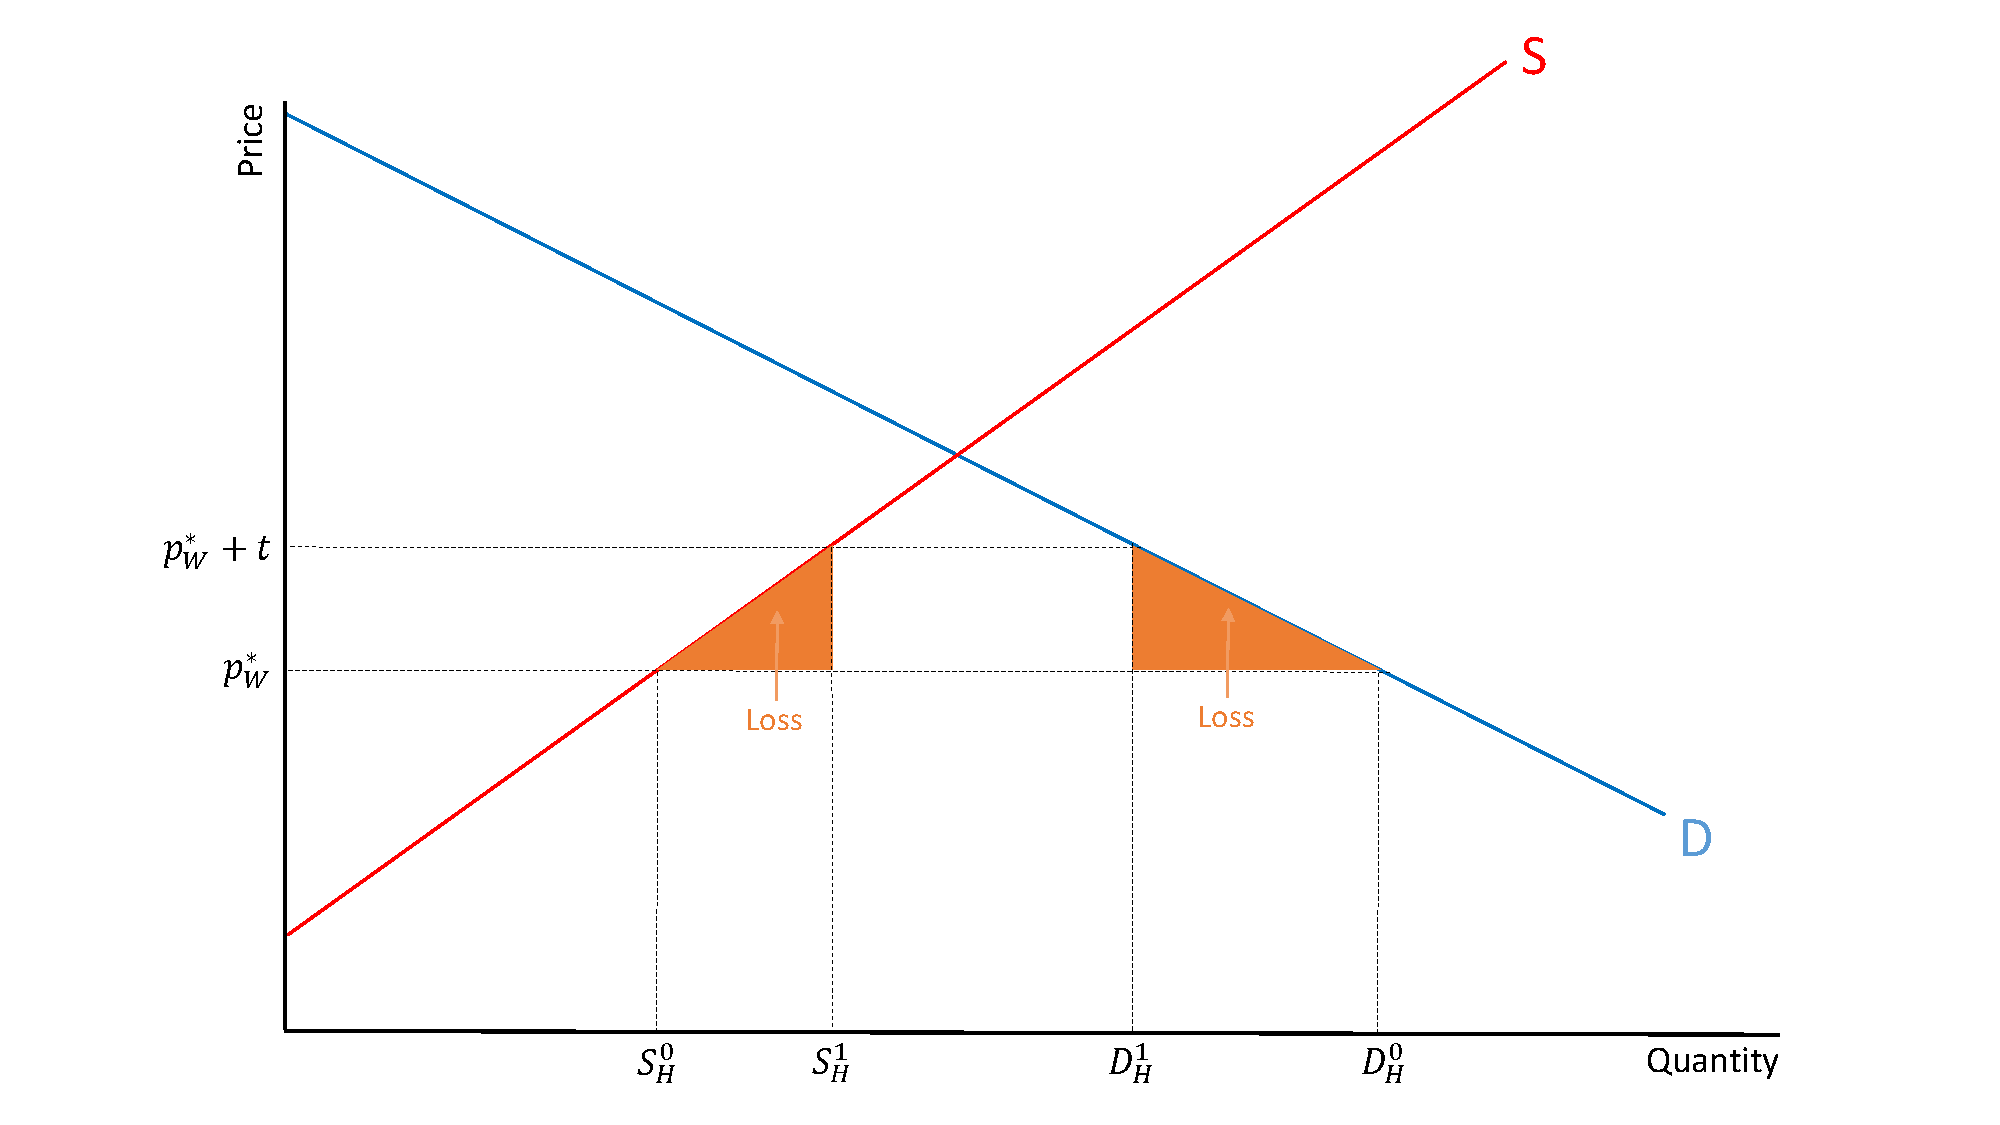
\includegraphics[scale=0.3]{SL_9.pdf}
\end{frame}

\subsection{Theory: Large country}

\begin{frame}
	\frametitle{Tariffs in a large open economy}
	\begin{itemize}
		\item Tariffs non-optimal for a small open economy!
		\item So why do we see them?
		\begin{itemize}
				\item Terms of trade considerations!
					\begin{itemize}
						\item Tariff barriers can drive down the world price of the import good, benefiting consumers.
						\item For this to be true, economy needs to be ``large" (i.e., its behaviour must affect world prices.)
					\end{itemize}
			\end{itemize}
		\item We now turn to a large country model to understand the potential benefits of tariff barriers.
	\end{itemize}
\end{frame}

\begin{frame}
	\frametitle{Free-Trade Equilibrium with a Large Open Economy}
	\begin{itemize}
		\item For simplicity, we suppose there are two large economies: Home ($H$) and Foreign ($F$) 
		\item Equilibrium free-trade price, $p_W$, is the price such that import demand from one country is equal to the export supply of the other country.
		\item Suppose Home imports, Foreign exports
		\item Equilibrium given by the following conditions:
			\begin{enumerate}
				\item Exports = Imports
								\begin{itemize}
									\item $D_H(p_w) - S_H(p_w) = S_F(p_w) - D_H(p_w)$
								\end{itemize}
			\item World Demand = World Supply
					\begin{itemize}
						\item $D_H(p_w) +  D_H(p_w) = S_H(p_w) + S_F(p_w)$ 
					\end{itemize}
			\end{enumerate}
		\item Note that (1) is just (2) rearranged, so we can use either condition to solve for equilibrium.
	\end{itemize}
\end{frame}

\begin{frame}
	\frametitle{Equilibrium with a Large Open Economy: Diagram}
	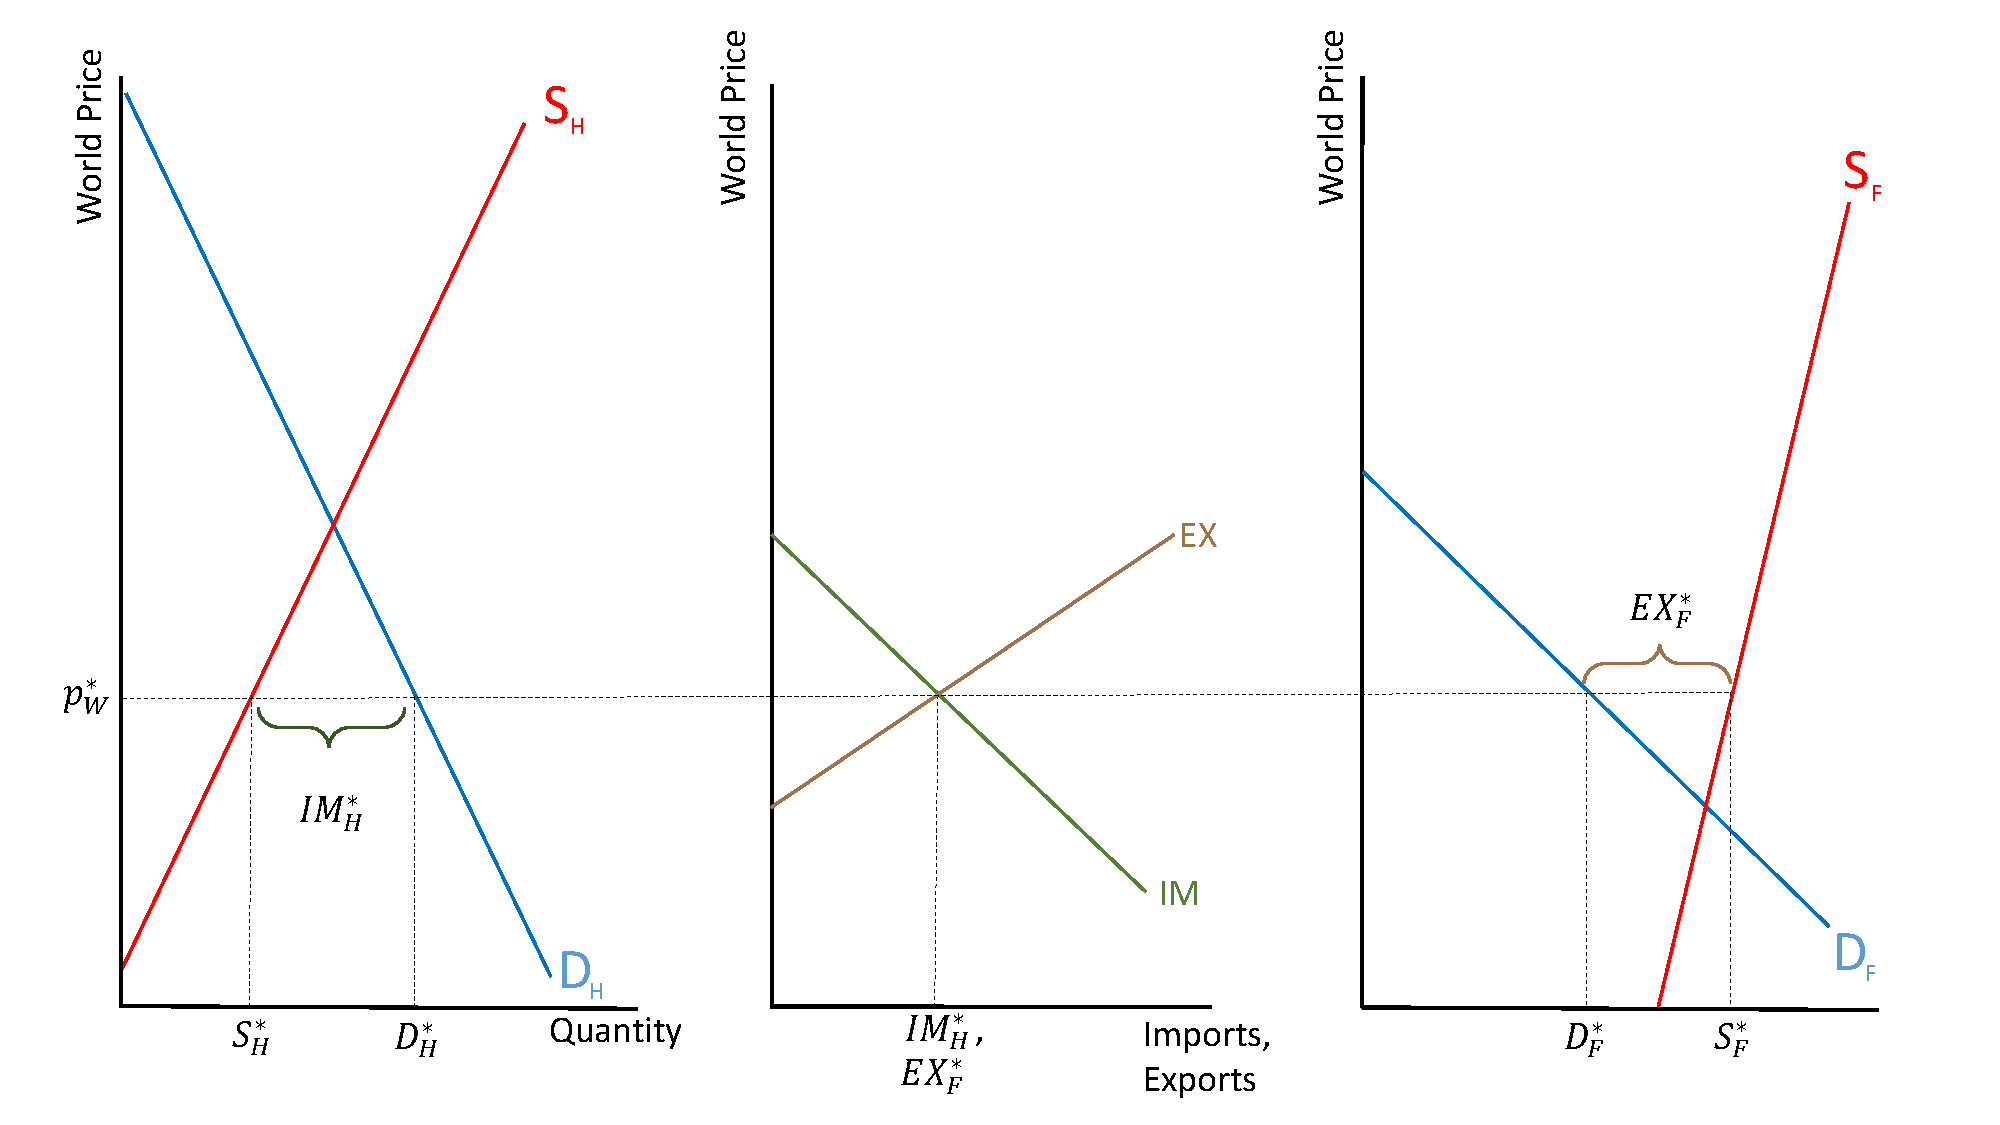
\includegraphics[scale=0.3]{SL_10.pdf}
\end{frame}

\begin{frame}
	\frametitle{Solving for Free Trade Prices and Quantities}
\begin{itemize}
	\item Need to know who will export and who will import.
		\begin{itemize}
			\item Solve for equilibrium prices \emph{in autarky}. The country with the lowest price will be the exporter.
				\begin{itemize}
					\item Why?
				\end{itemize}
	\item Solve for Import Demand $D_i - S_i$ and Export Supply $S_j-D_j$ curves.
	\item Set Import Demand equal to Export Supply, solve for prices.
	\item Substitute prices back in to Import Demand (or Export Supply) to get trade levels.
		\end{itemize}\vspace{4mm}
Note: Can also use World Demand = World Supply Condition
\end{itemize}
\end{frame}

\begin{frame}
	\frametitle{Effect of Tariff for Large Open Economy.}
	\begin{itemize}
		\item Specific tariff, $t$, introduces a wedge between the \emph{Foreign} price ($p_F$) and the \emph{Home} price ($p_H$).
		\begin{itemize}
			\item If we have two countries with two different prices, not clear what the world price is.
			\item Instead of one endogenous world price, we have two endogenous \emph{local} prices.
		\end{itemize}
	\item Equilibrium condition
		\begin{itemize}
		\item Exporters (Foreign Suppliers) still need to be compensated for the extra cost associated with selling in the Home market.
		\begin{itemize}
			\item Must be that $p_H-t=p_F$ or $p_H = p_F + t$
		\end{itemize}
	\end{itemize}
	\end{itemize}
\end{frame}

\begin{frame}
	\frametitle{Effect of Tariff for large Open Economy}
Since $p_H=p_F+t$, effective price at home needs to be higher for every candidate value of $p_F$.
	\begin{itemize}
		\item Can be represented as a shift inwards in the import demand curve, treating $p_F$ as the new ``world price"
		\begin{itemize}
			\item Mathematically: Instead of taking $p_W$ as given, take $p_F+t$ as given, and re-derive import demand curve.
			\begin{itemize}
				\item $IM_H(p_F+t)=D_H(p_F+t) - S_H(p_F+t) $
				\item Note: Before tariff: $p_W=p_F$
			\end{itemize}
			\item Side Note: Could instead treat $p_H$ as the world price, in which case the export supply curve shifts.
		\end{itemize}
	\end{itemize}
\end{frame}

\begin{frame}
	\frametitle{Effect of Tariff for Large Open Economy}
	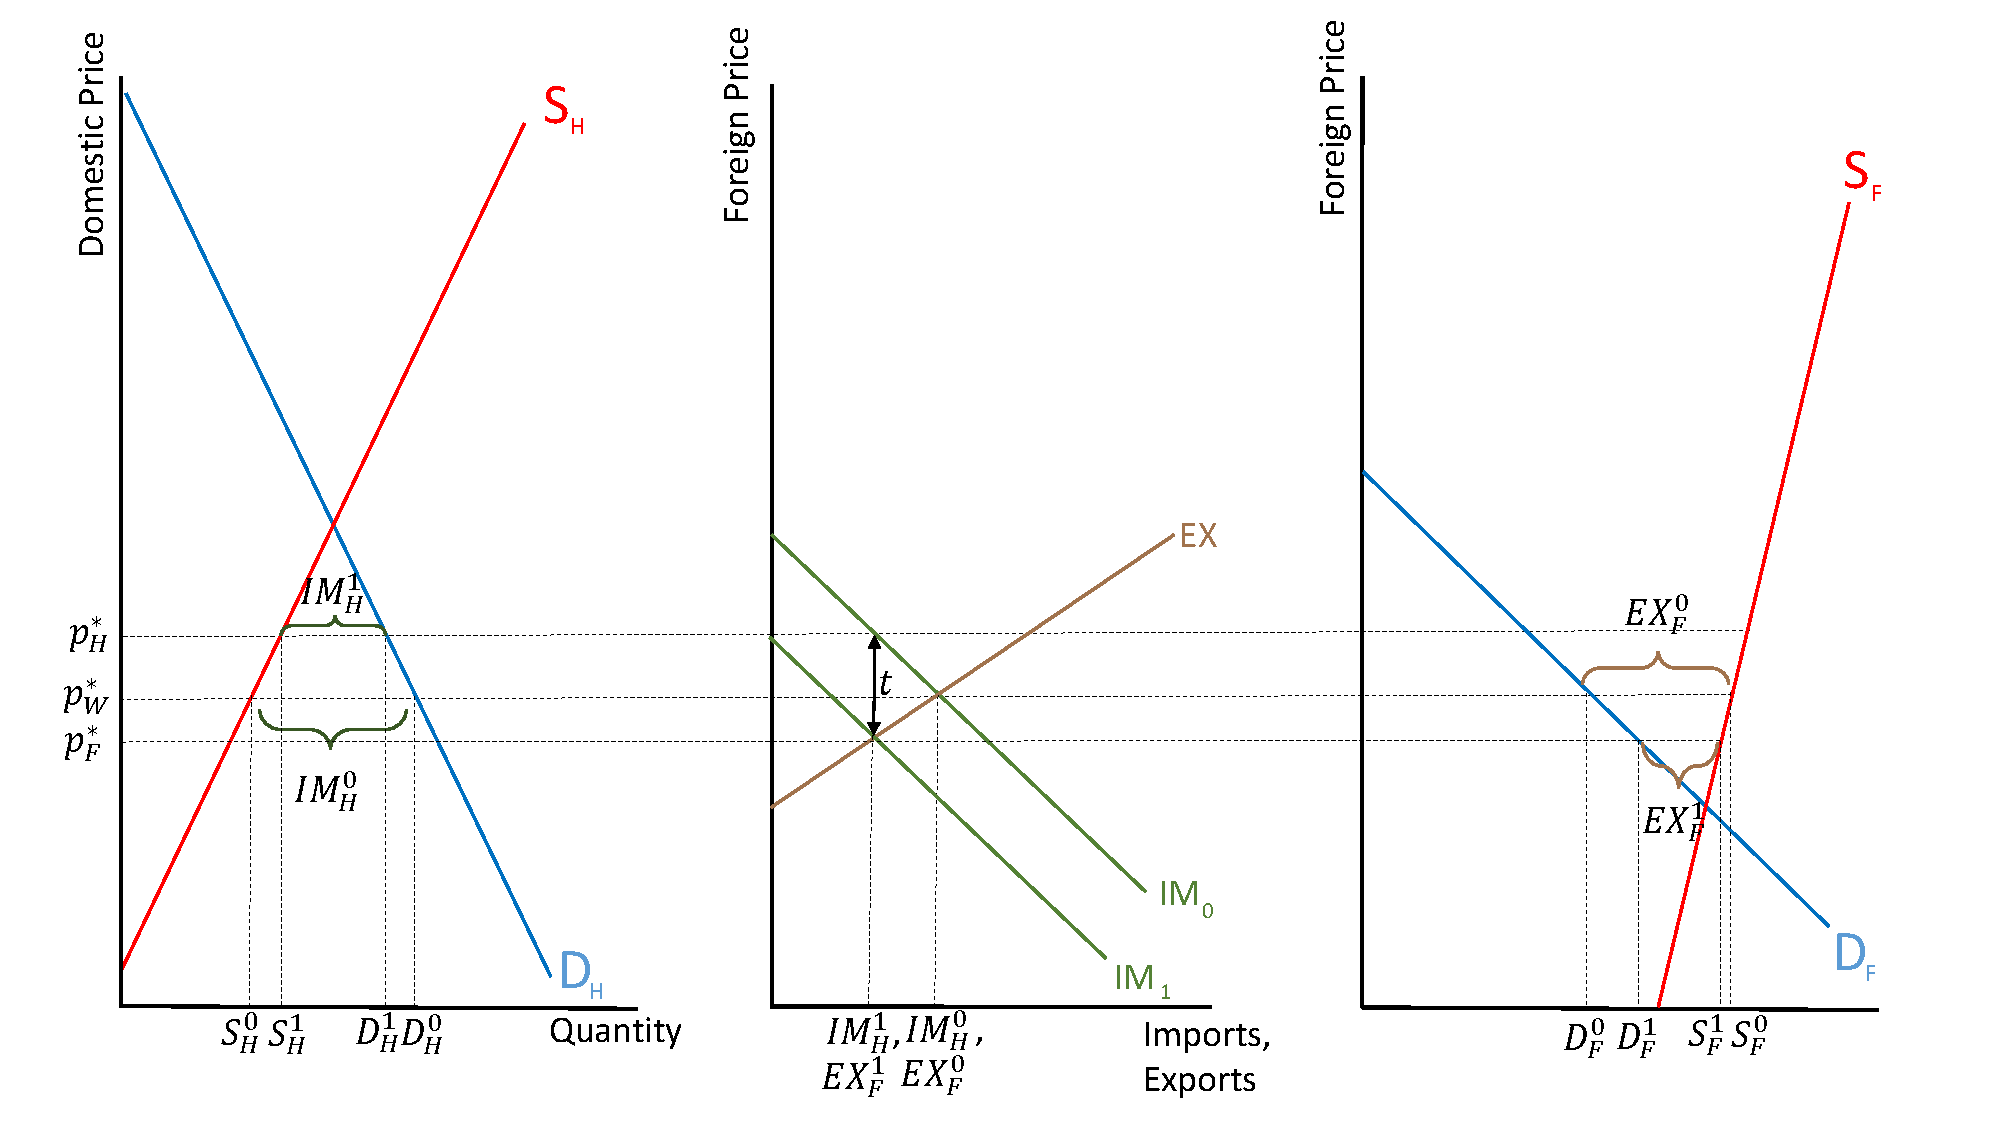
\includegraphics[scale=0.3]{SL_11.pdf}
\end{frame}

\begin{frame}
	\frametitle{Solving For Prices and Quantities with Tariffs}
	
	\begin{itemize}
		\item Solve for equilibrium $p_F$
			\begin{itemize}
				\item Set new $IM_H(p_F+t)=D_H(p_F+t) - S_H(p_F+t) $ equal to $EX_F(p_F)$, and solve.
			\end{itemize}
		\item Must have $p_H = p_F + t$
		\item Trade flows obtained by substituting $p_F$ into $EX_F(p_F)$
		\item Quantities demand and supplied obtained by plugging the appropriate price into the demand and supply functions.
	\end{itemize}

\end{frame}

\begin{frame}
	\frametitle{Effect of Tariff for Large Open Economy}
	\begin{itemize}
		\item Imports fall, as in the open economy case.
		\item However, the foreign price of the good \emph{falls}.
		\item Wedge between foreign and home price generates a \emph{terms-of-trade gain} 
			\begin{itemize}
				\item Fall in foreign price means imports are cheaper for the country.
				\item While the price consumers pay domestically is actually higher, the gains from cheaper imports show up in the tariff revenue.
					\begin{itemize}
						\item Government revenue can be transferred to consumers, so acts as a wealth effect.
					\end{itemize}
			\end{itemize}
	\end{itemize}
\end{frame}

\begin{frame}
	\frametitle{Tariffs in Large Open Economies:  Pre-Tarif Surplus}
	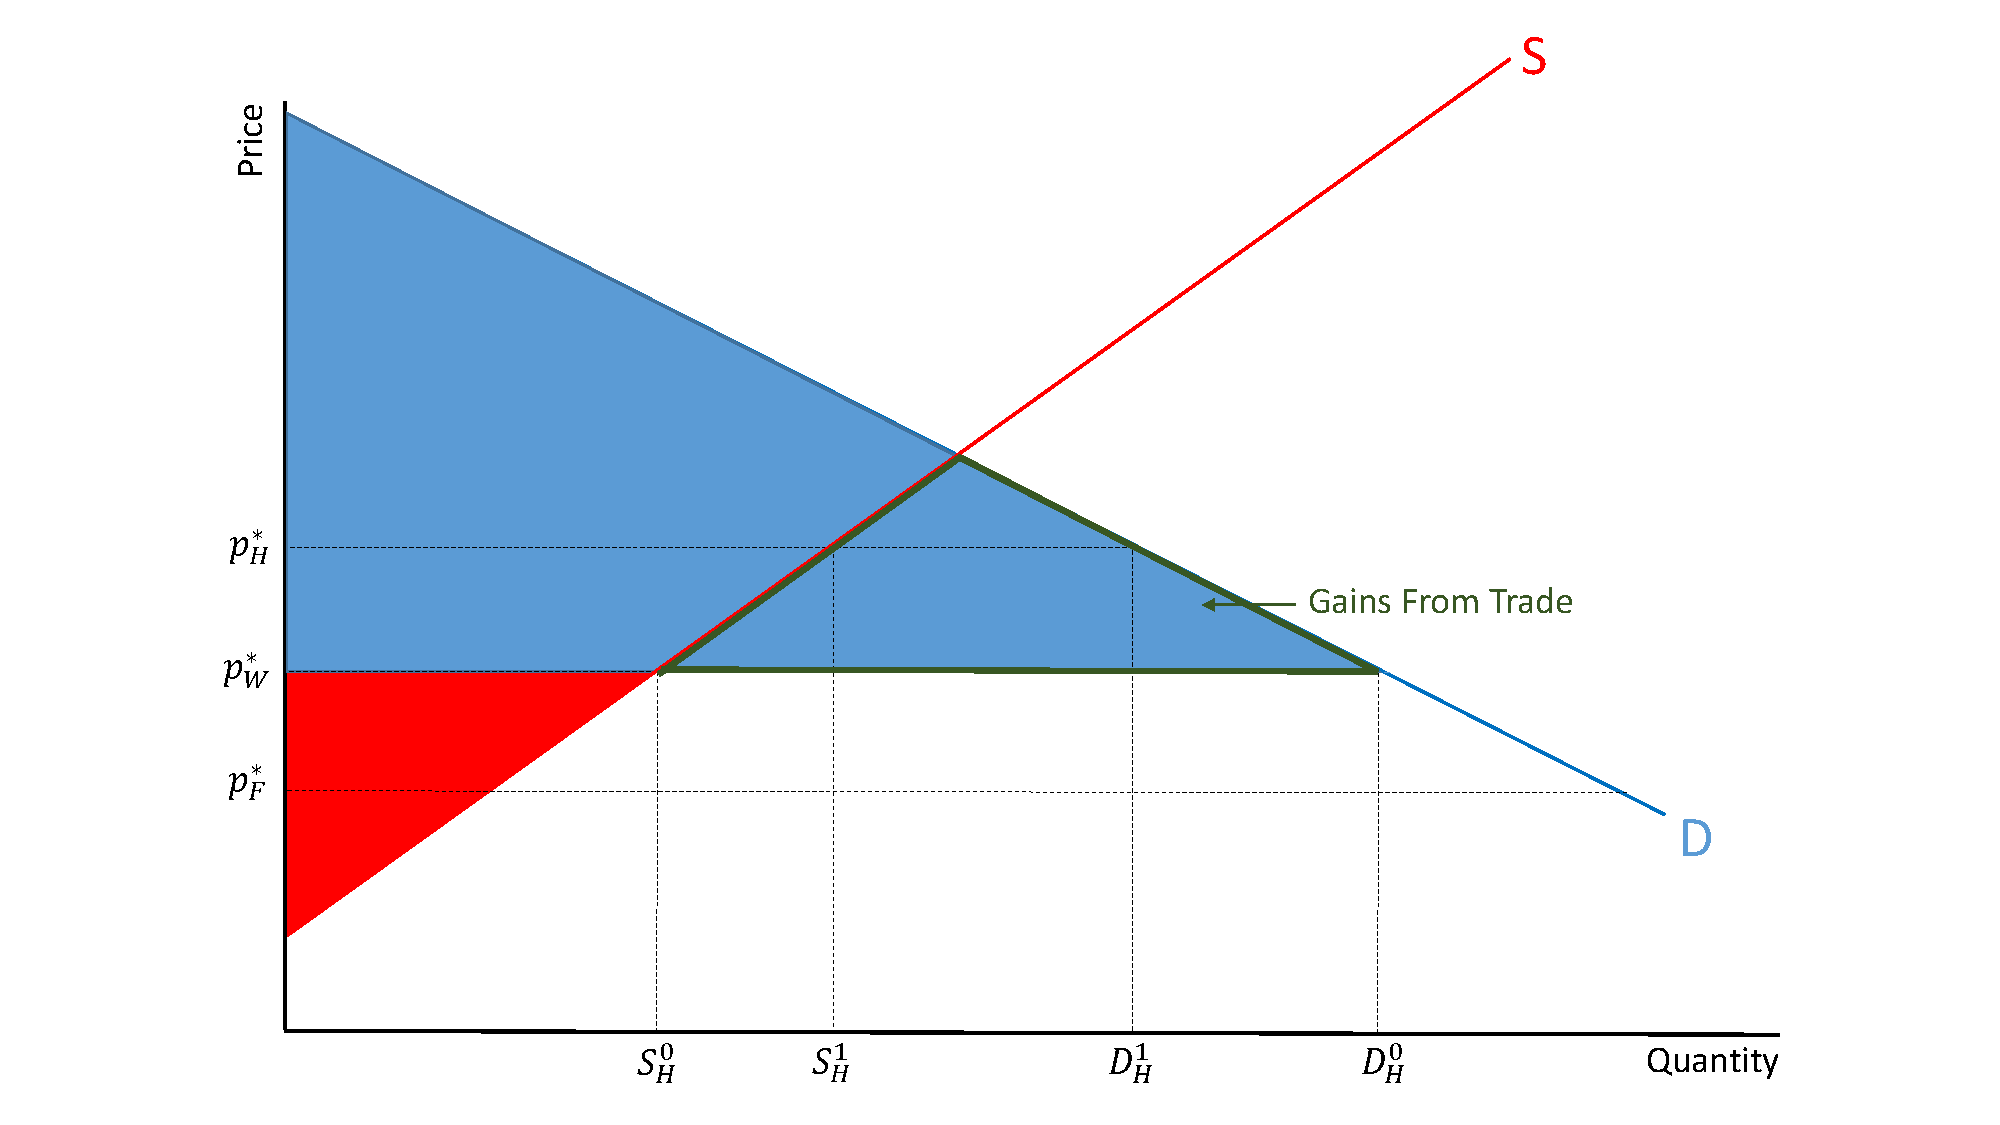
\includegraphics[scale=0.3]{SL_12.pdf}

	
\end{frame}

\begin{frame}
	\frametitle{Tariffs in Large Open Economies:  Post-Tarif Surplus}
	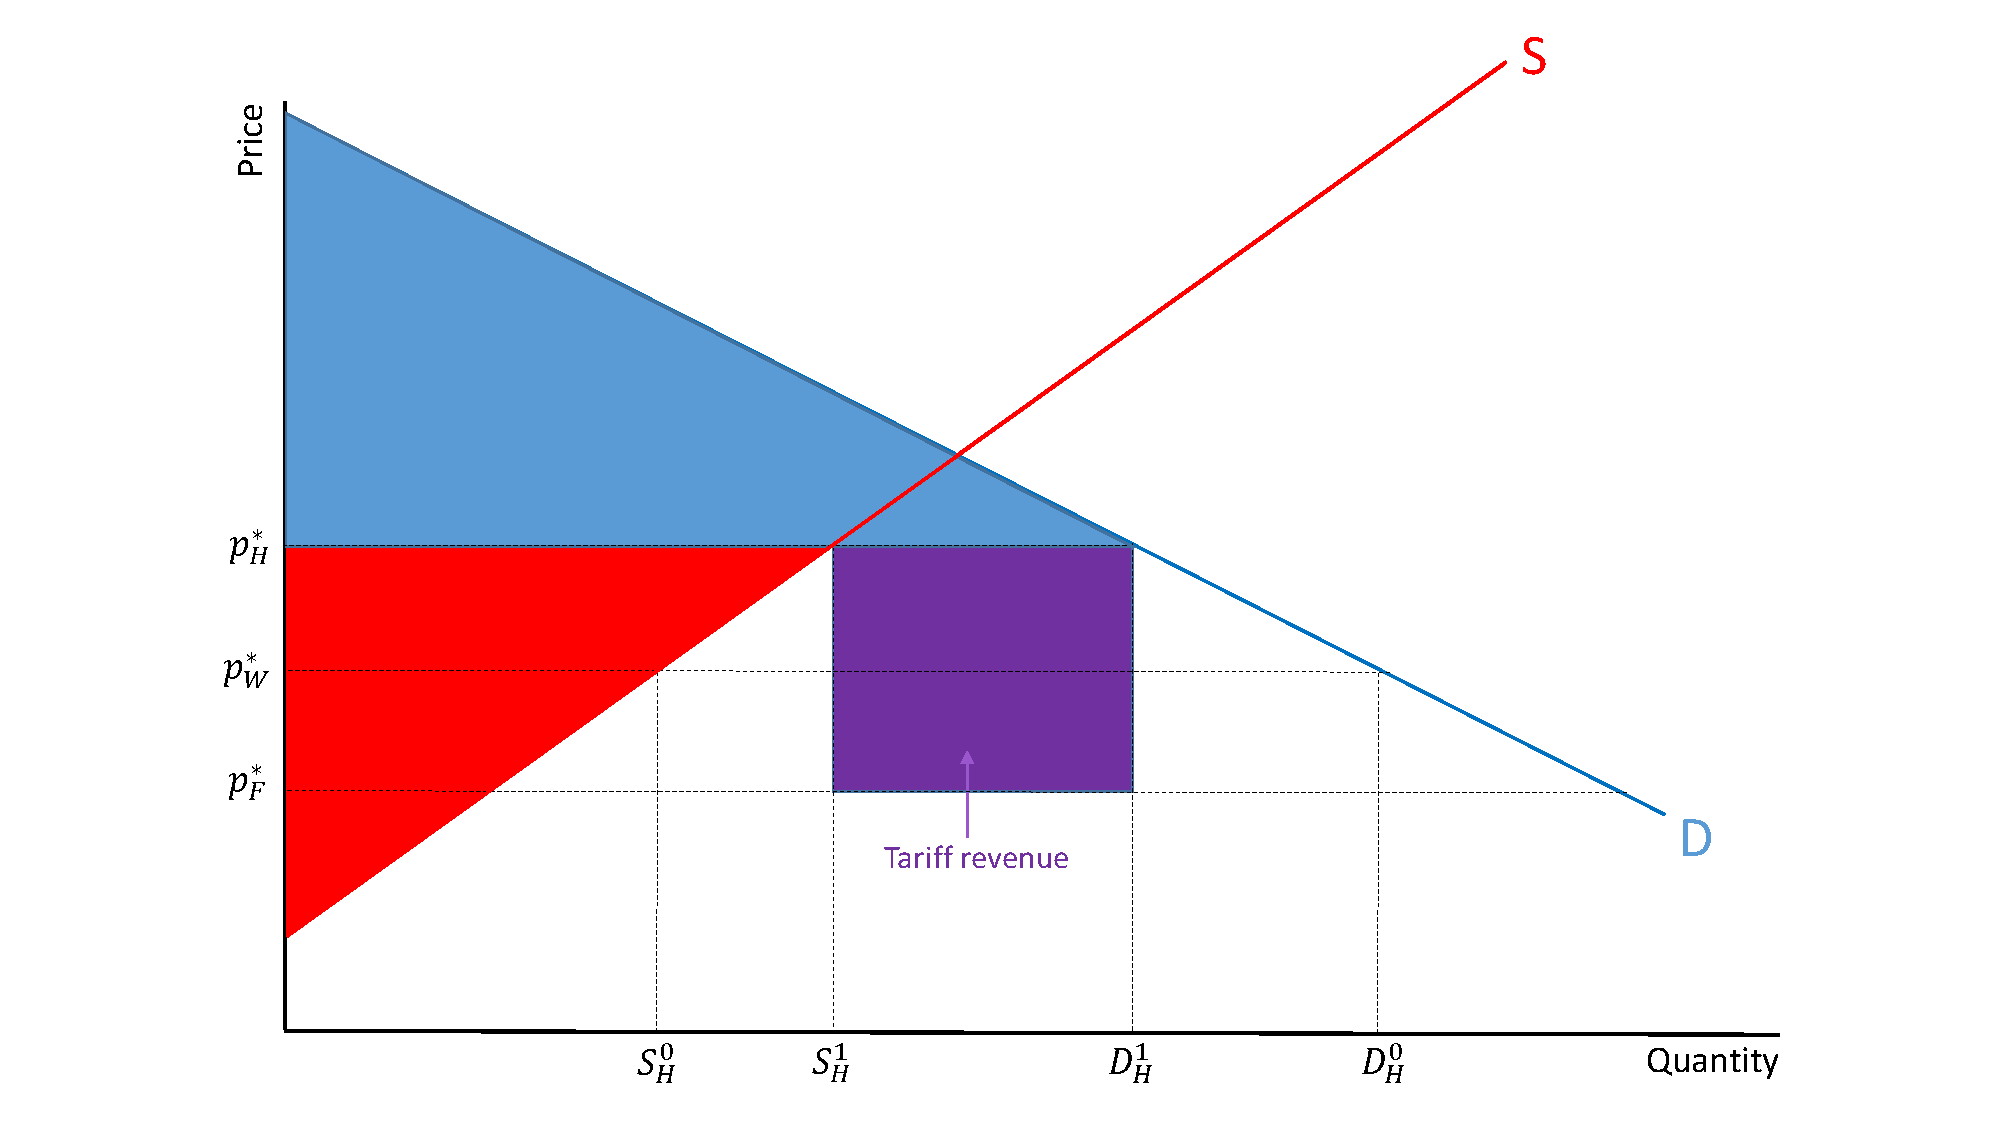
\includegraphics[scale=0.3]{SL_13.pdf}
	
	
\end{frame}

\begin{frame}
	\frametitle{Tariffs in Large Open Economies: Net Surplus}
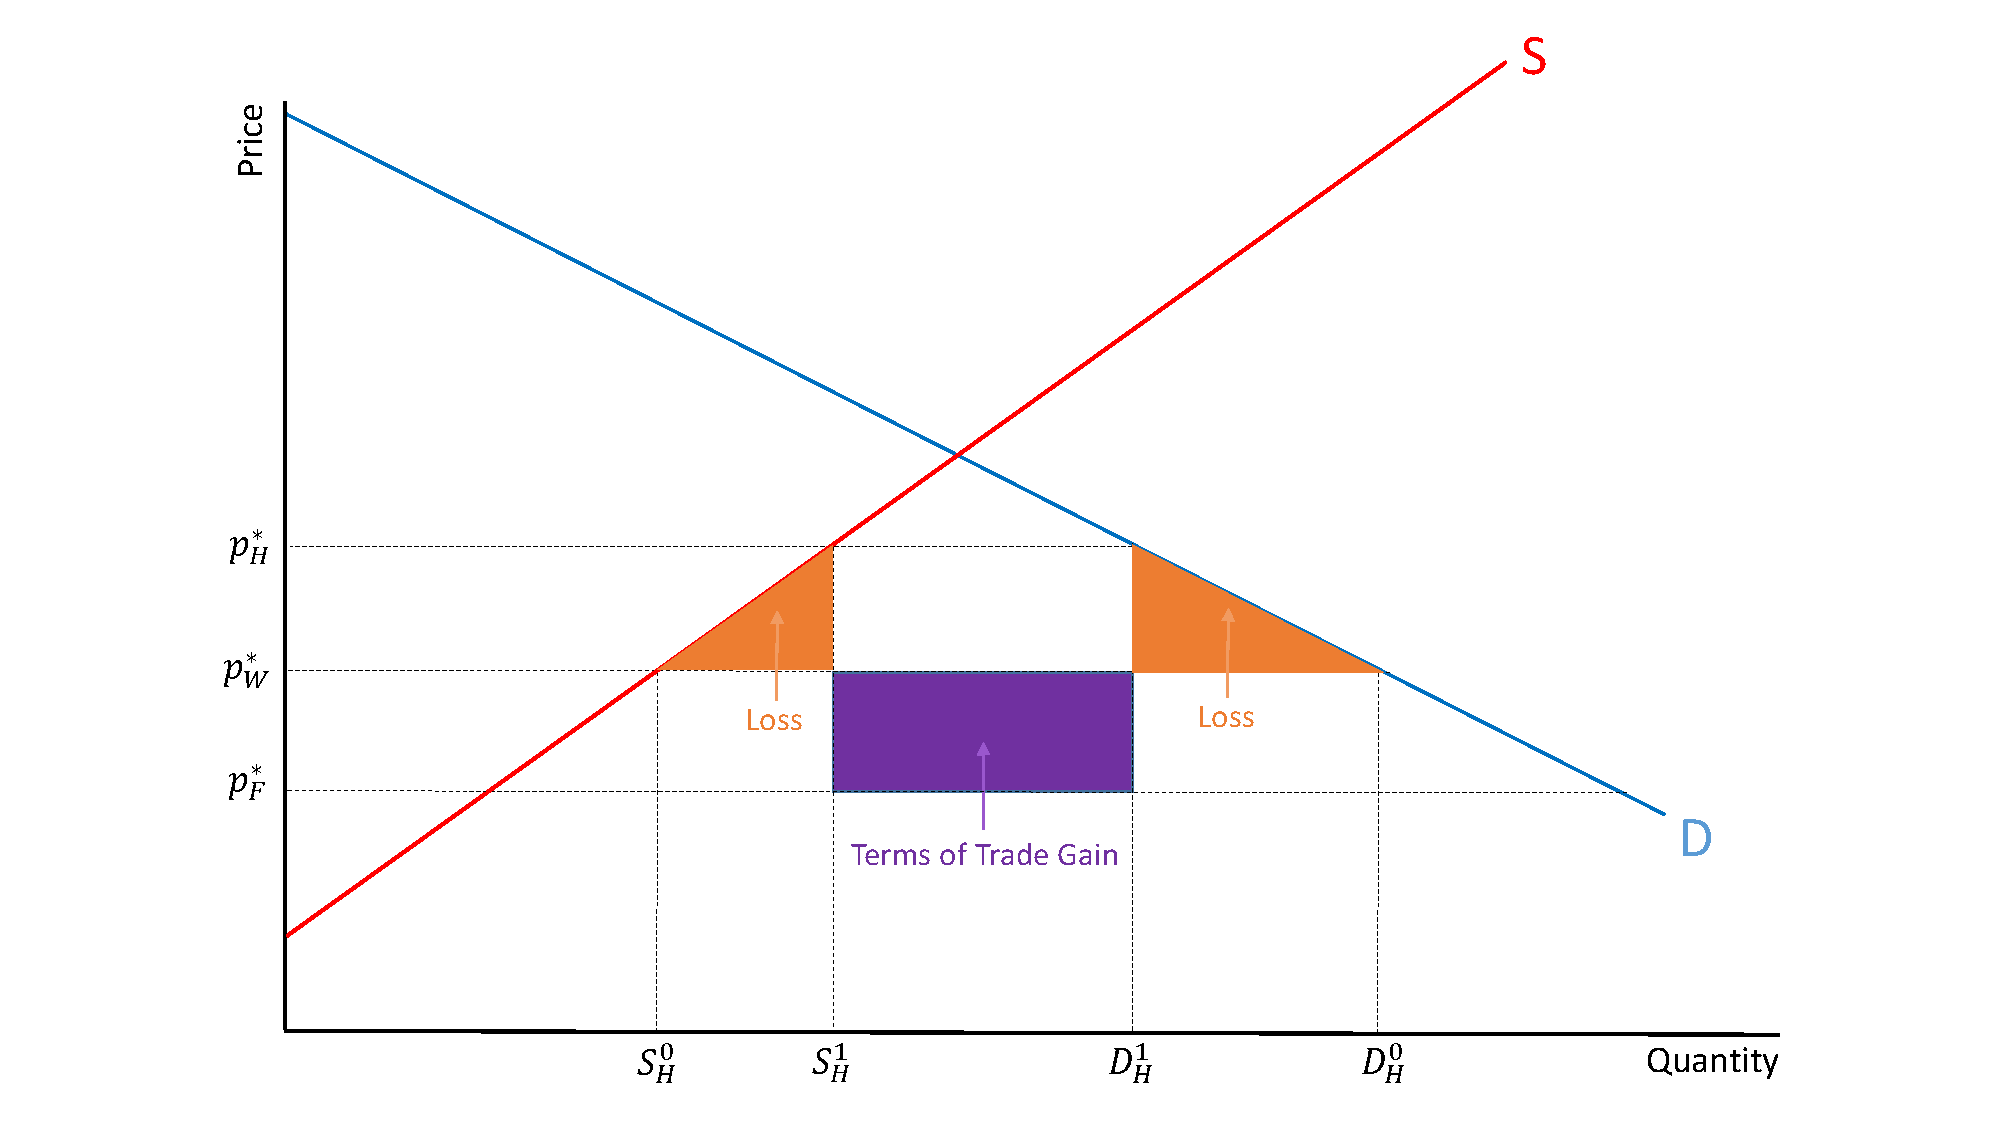
\includegraphics[scale=0.3]{SL_14.pdf}

\end{frame}

\begin{frame}
	\frametitle{Can Tariffs Increase Welfare?}
	\begin{itemize}
		\item Existence of the \emph{terms of trade gains} means that tariffs \emph{could} lead to welfare gains.
			\begin{itemize}
				\item Is the purple region ever bigger than the two orange regions?
			\end{itemize}
		\item We shall now see that there will indeed be welfare gains for some positive levels of tariffs.
				\begin{itemize}
					\item Can we find the \emph{optimal tariff}?
						\begin{itemize}
							\item Straightforward to do when demand and supply are linear.
						\end{itemize}
				\end{itemize}
		\item Reference: Appendix to Chapter 10 in KOM.
	\end{itemize}
\end{frame}

\begin{frame}
	\frametitle{Calculating Welfare}
	
	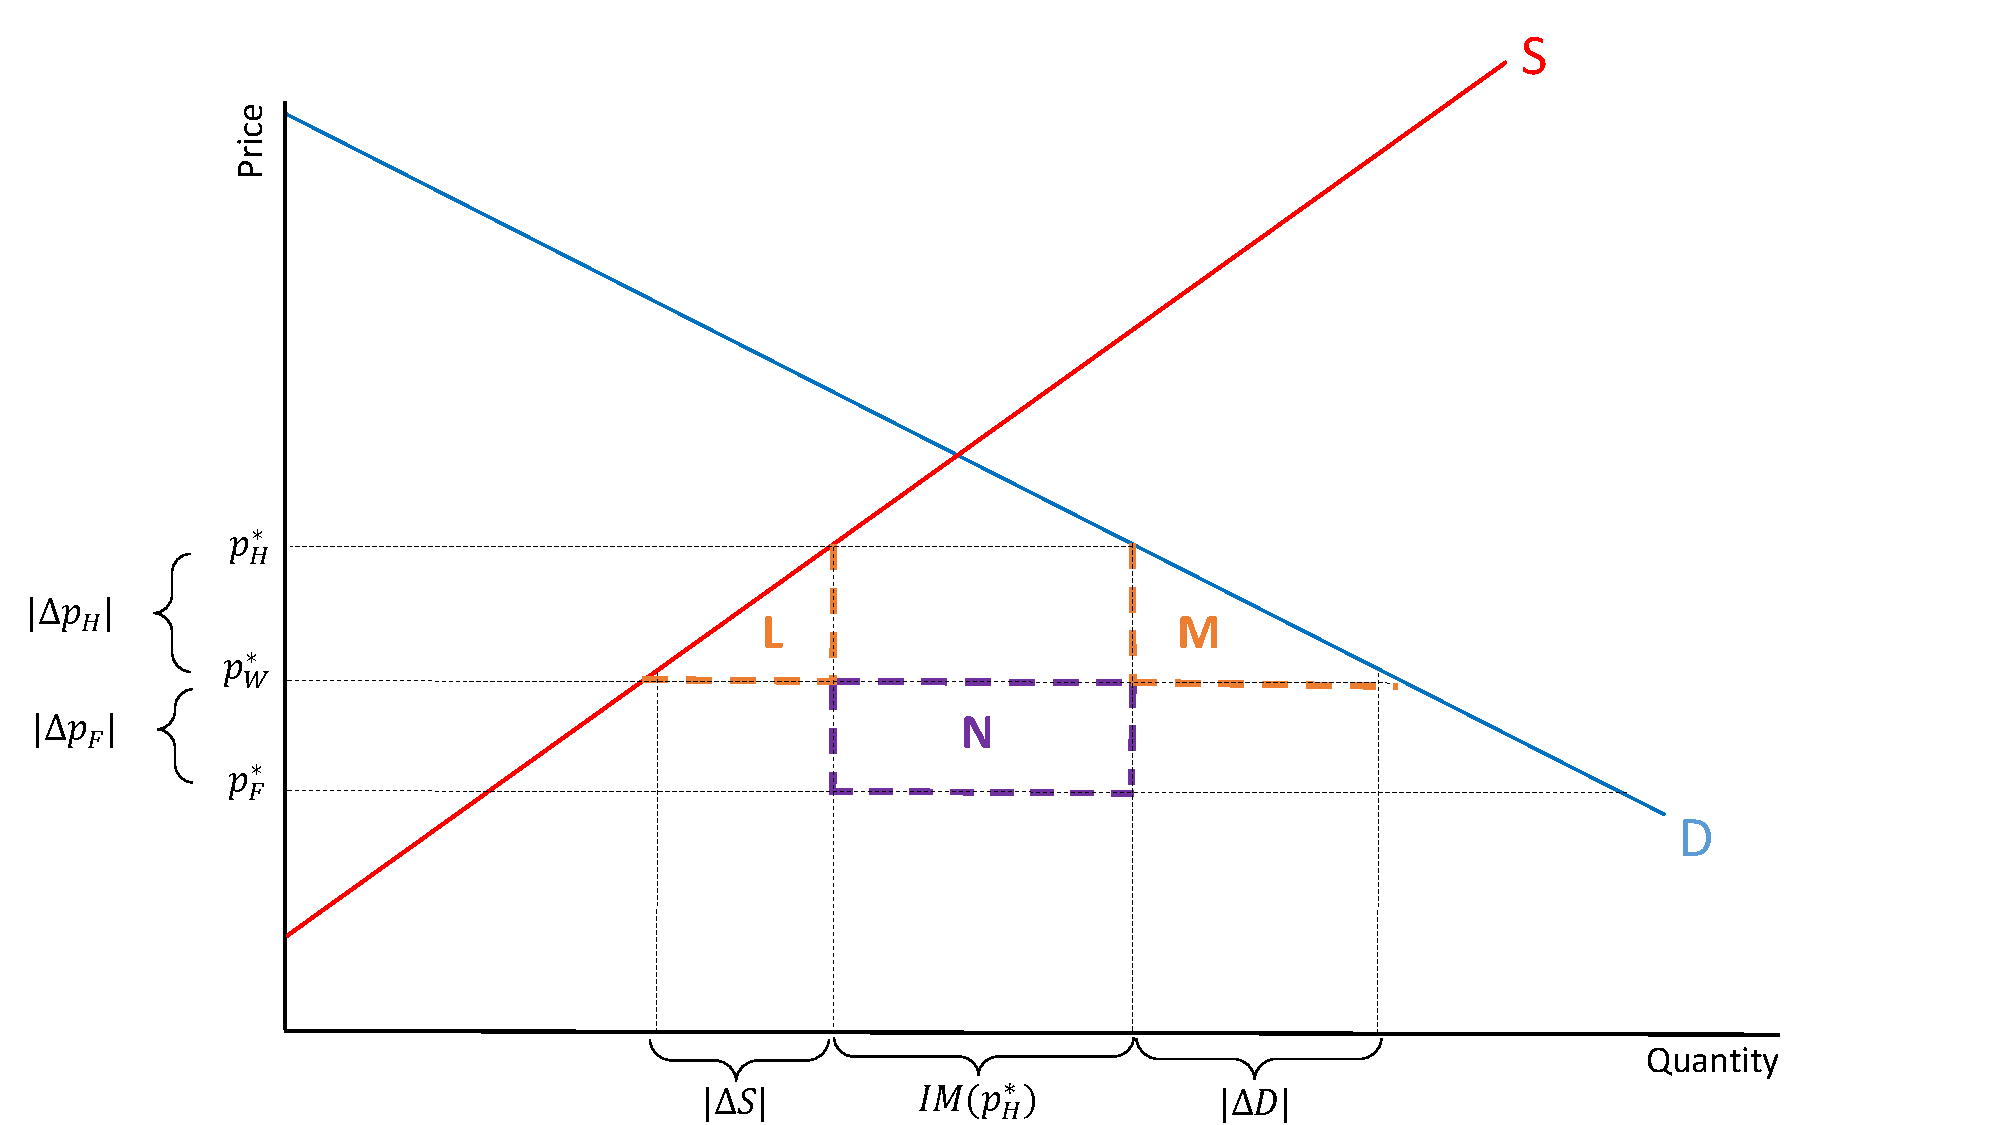
\includegraphics[scale=0.3]{SL_15.pdf}
	
\end{frame}

\begin{frame}
	\frametitle{Can Tariffs Increase Welfare?}
\scriptsize
Suppose:
	\begin{itemize}
		\scriptsize
		\item Home Demand: $D_H(p) = A - B\times p$ 
		\item Home Supply: $S_H(p)  = C\times p$ 
		\item Export Supply: $EX_F = J + K\times p_F=J + K\times (p_H-t)$ 
\end{itemize}
		
Solve for equilibrium prices with free trade and without:
	\begin{itemize}
		\scriptsize
		\item $p^*_w=\frac{A-J}{B+C+K}$ 
		\item $p^*_H=p^*_w + \frac{K}{B+C+K}\times t \rightarrow |\Delta p_H| =\frac{K}{B+C+K}\times t $ 
		\item $p^*_F=p^*_w-\frac{B+C}{B+C+K}\times t  \rightarrow |\Delta p_F| =\frac{B+C}{B+C+K}\times t $ 
	\end{itemize}
Also note:
	\begin{itemize}
		\scriptsize
		\item $|\Delta D| = D_H(p^*_W) - D_H(p^*_H)  =B\times\left(p^*_H -\ p^*_w\right)= \frac{BK}{B+C+K}\times t$ 
		\item $|\Delta S|  = S_H(p^*_H) - S_H(p^*_W) =C\times\left(p^*_H - p^*_w\right)=\frac{CK}{B+C+K}\times t$
		\item $IM(p^*_H)=(A) - (B+C)\times p_H =A - \left(\frac{B+C}{B+C+K}\right)\left(A-J + K\times t\right)$
	\end{itemize}
\end{frame}


\begin{frame}
	\frametitle{Can Tariffs Increase Welfare?}
	\scriptsize

	\begin{itemize}
		\scriptsize
		\item  Part L:  $\frac{1}{2}|\Delta p_H|\times |\Delta S|=\frac{C}{2}\left(\frac{K}{B+C+K}\right)^2\times t^2$ 
		\item  Part M: $\frac{1}{2}|\Delta p_H|\times |\Delta D|= \frac{B}{2}\left(\frac{K}{B+C+K}\right)^2\times t^2$ 
		\item  Part N: $|\Delta p_F| \times IM(p_H)=\frac{B+C}{B+C+K}\times t\times\left(A - \left(\frac{B+C}{B+C+K}\right)\left(A-J + K\times t\right)\right)$ 
	\end{itemize}
Total change in Welfare given by:
	\begin{itemize}
		\scriptsize
		\item  $\Delta W$ = Part N - Part L - Part M
	\end{itemize}
\vspace{3mm}Can Show:
\begin{equation}
\Delta W = Xt - Zt^2 \nonumber
\end{equation}
	\begin{itemize}
		\item Where:
			\begin{itemize}
				\item $X =\frac{(B+C)(AK+JB+JC)}{\left(B+C+K\right)^2}$
				\item $Z = \frac{K(B+C)\left(2B+2C + K \right)}{2\left(B+C+K\right)^2}$
			\end{itemize}
	\end{itemize}

\end{frame}

\begin{frame}
	\frametitle{Can Tariffs Increase Welfare?}
\begin{equation}
\Delta W = Xt - Zt^2 \nonumber
\end{equation}
\begin{itemize}
	\item Note that the change in welfare is a quadratic in $t$ 
	\item Since $Z>0$ (see previous slide), this function is \emph{concave} in $t$, so there is a global maximum for some finite $t$
	\item Is the maximum somewhere with $t>0$?
		\begin{itemize}
			\item Take FOC for maximum:
				\begin{itemize}
					\item $X - 2Zt^*=0 \rightarrow t^*= \frac{X}{2Z}$ 
				\end{itemize}
			\item Yes, since $X>0$.
			
		\end{itemize}
\end{itemize}
\begin{center}
	A large open economy can be better off if they choose to implement an (optimal) positive tariff!
\end{center}

\end{frame}
\begin{frame}
	\frametitle{Tariffs and World Welfare}
\begin{itemize}
	\item While introducing a tariff barrier increases the welfare of Home, it \emph{hurts} Foreign.
		\begin{itemize}
			\item You are asked to show this in assignment 3.
		\end{itemize}
	\item Introducing tariffs problematic for \emph{world} welfare.
	\begin{itemize}
				\item Governments trying to maximize the welfare of their own citizens do not account for the welfare cost on foreign citizens.
	\end{itemize}
	
	\item Moreover, note that by a similar argument, Foreign will want to put a tariff on their imports as well!
		\begin{itemize}
			\item Incentive for trade wars! 
			\item More on this later... (Chapter 10)
		\end{itemize}

\end{itemize}
\end{frame}

\begin{frame}
	\frametitle{A note on the optimal tariff and export supply}
\footnotesize
\begin{center}
		\begin{equation}
		EX_F = J + K\times p_F=J + K\times (p_H-t) \nonumber
		\end{equation}
	\begin{equation}
	 t^*= \frac{X}{2Z}=\frac{AK+J(B+C)}{K(2(B+C)+K)} =\frac{A}{2(B+C)+K}+\frac{J(B+C)}{K(2(B+C)+K)} \nonumber
	\end{equation}
\end{center}

\begin{itemize}
	\item Note that the optimal tariff falls as $K$ rises.
		\begin{itemize}
			\item The more response exports are to price, the \emph{less} you want to use tariffs.
				\begin{itemize}
					\item Why? Less market power!
				\end{itemize}
			\item For \emph{ad-valorem} tariffs, possible to show that in many environments the optimal tariff is given by the reciprocal of the export supply elasticity.
				\begin{itemize}
					\item See Broda, Limao and Weinstein (2008)
				\end{itemize} 
		\end{itemize}
\end{itemize}
	
	
	
\end{frame}

\section{Other Instruments}

\subsection{Export Subsidies}

\begin{frame}
	\frametitle{Export Subsidies}
	\textbf{Export Subsidies}: A payment to firms for shipping a good abroad
	\begin{itemize}
		\item Essentially the opposite of a tariff.
		\item Again, we only consider the impact of specific export subsidies, rather than \emph{ad-valorem} subsidies.
			\begin{itemize}
				\item Revenue per exported good: $(p+s)q$
			\end{itemize}
	\end{itemize}

Suppose Foreign introduces an export subsidy (Where both Home and Foreign are ``large").
		\begin{itemize}
			\item Subsidy introduces a wedge between foreign and home price.
				\begin{itemize}
					\item $p_F=p_H+s$
				\end{itemize}
		\end{itemize}
	
\end{frame}

\begin{frame}
	\frametitle{Export Subsidies}
	
	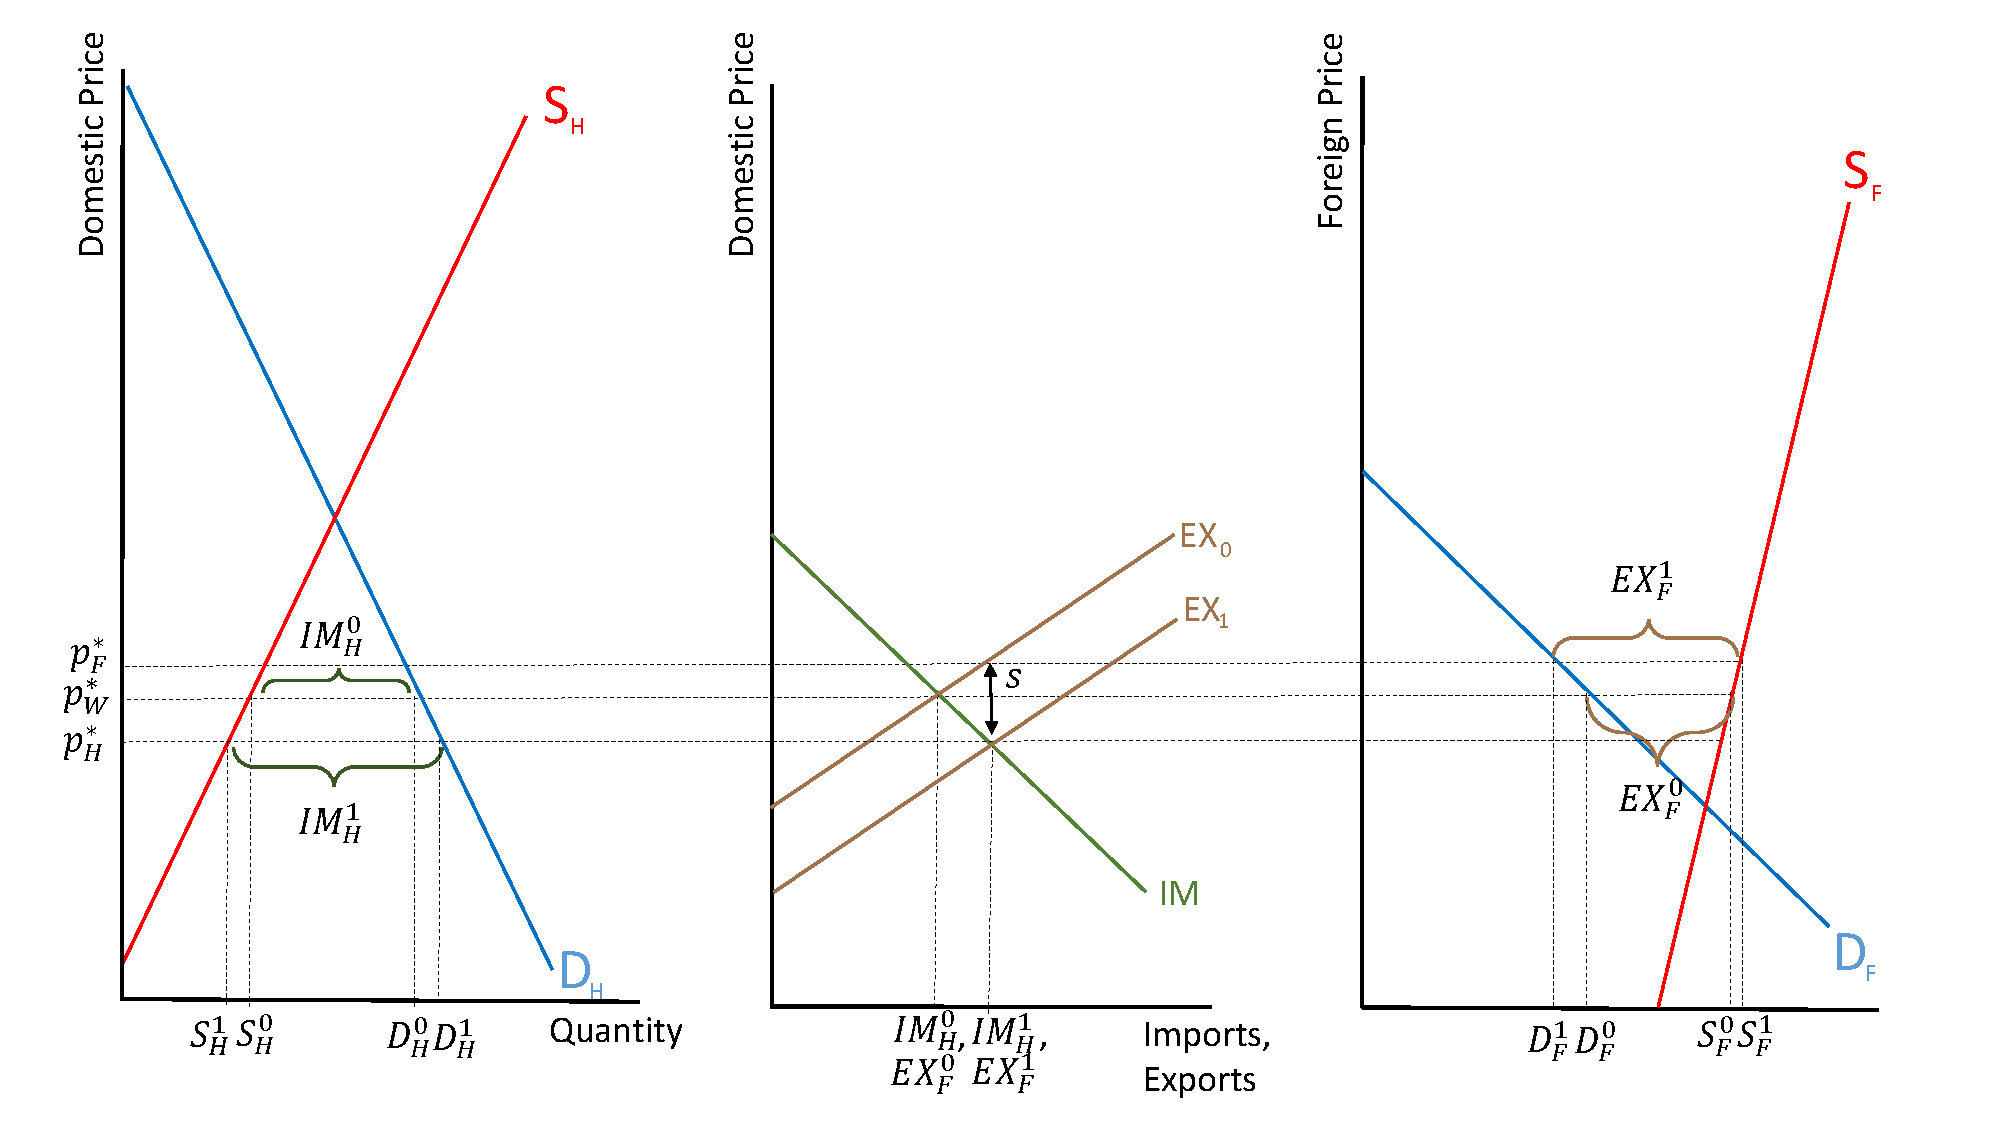
\includegraphics[scale=0.3]{SL_23.pdf}
	
\end{frame}


\begin{frame}
	\frametitle{Export Subsidies and Foreign Welfare: Surplus pre-subsidy}
	
	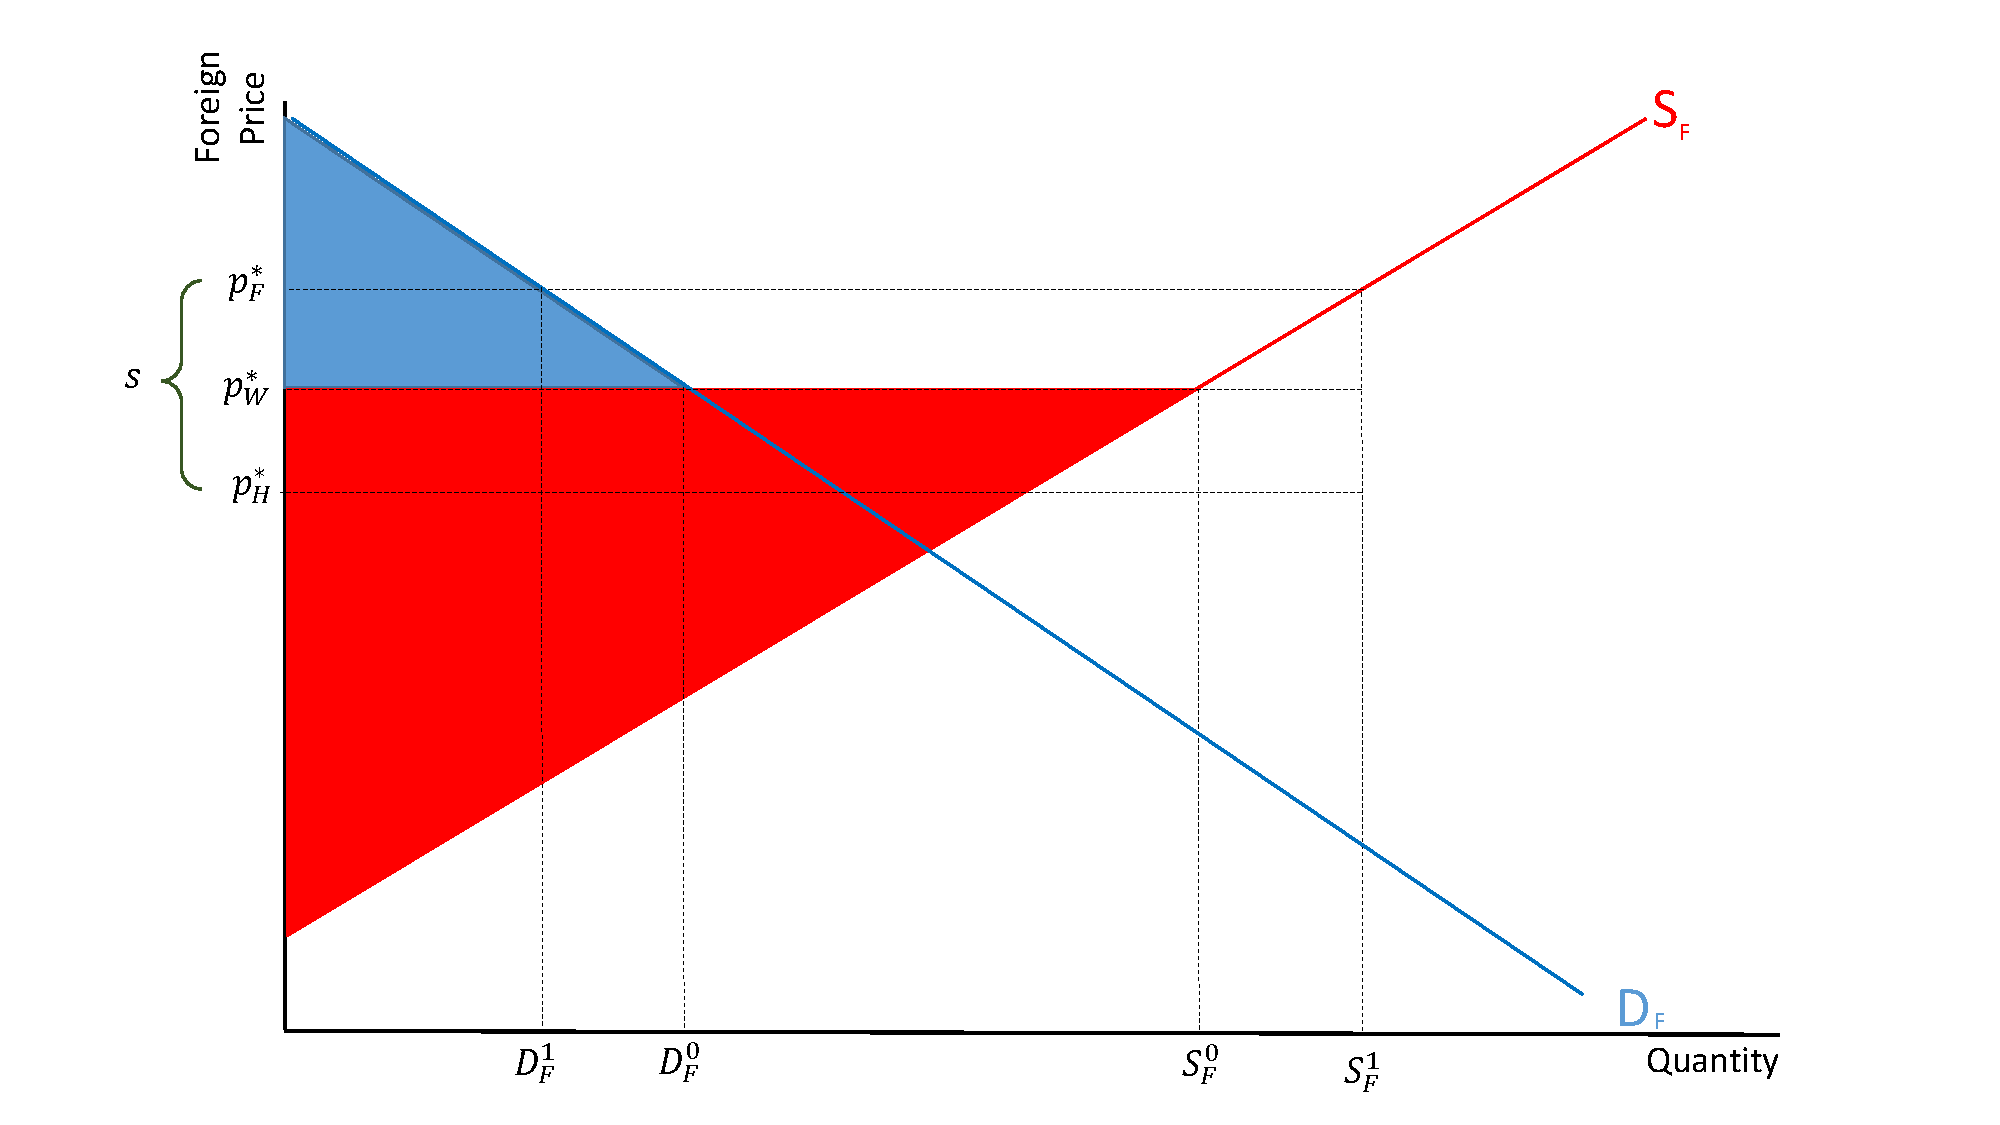
\includegraphics[scale=0.3]{SL_24.pdf}
	
\end{frame}

\begin{frame}
	\frametitle{Export Subsidies and Foreign Welfare: Surplus post-subsidy}
	
	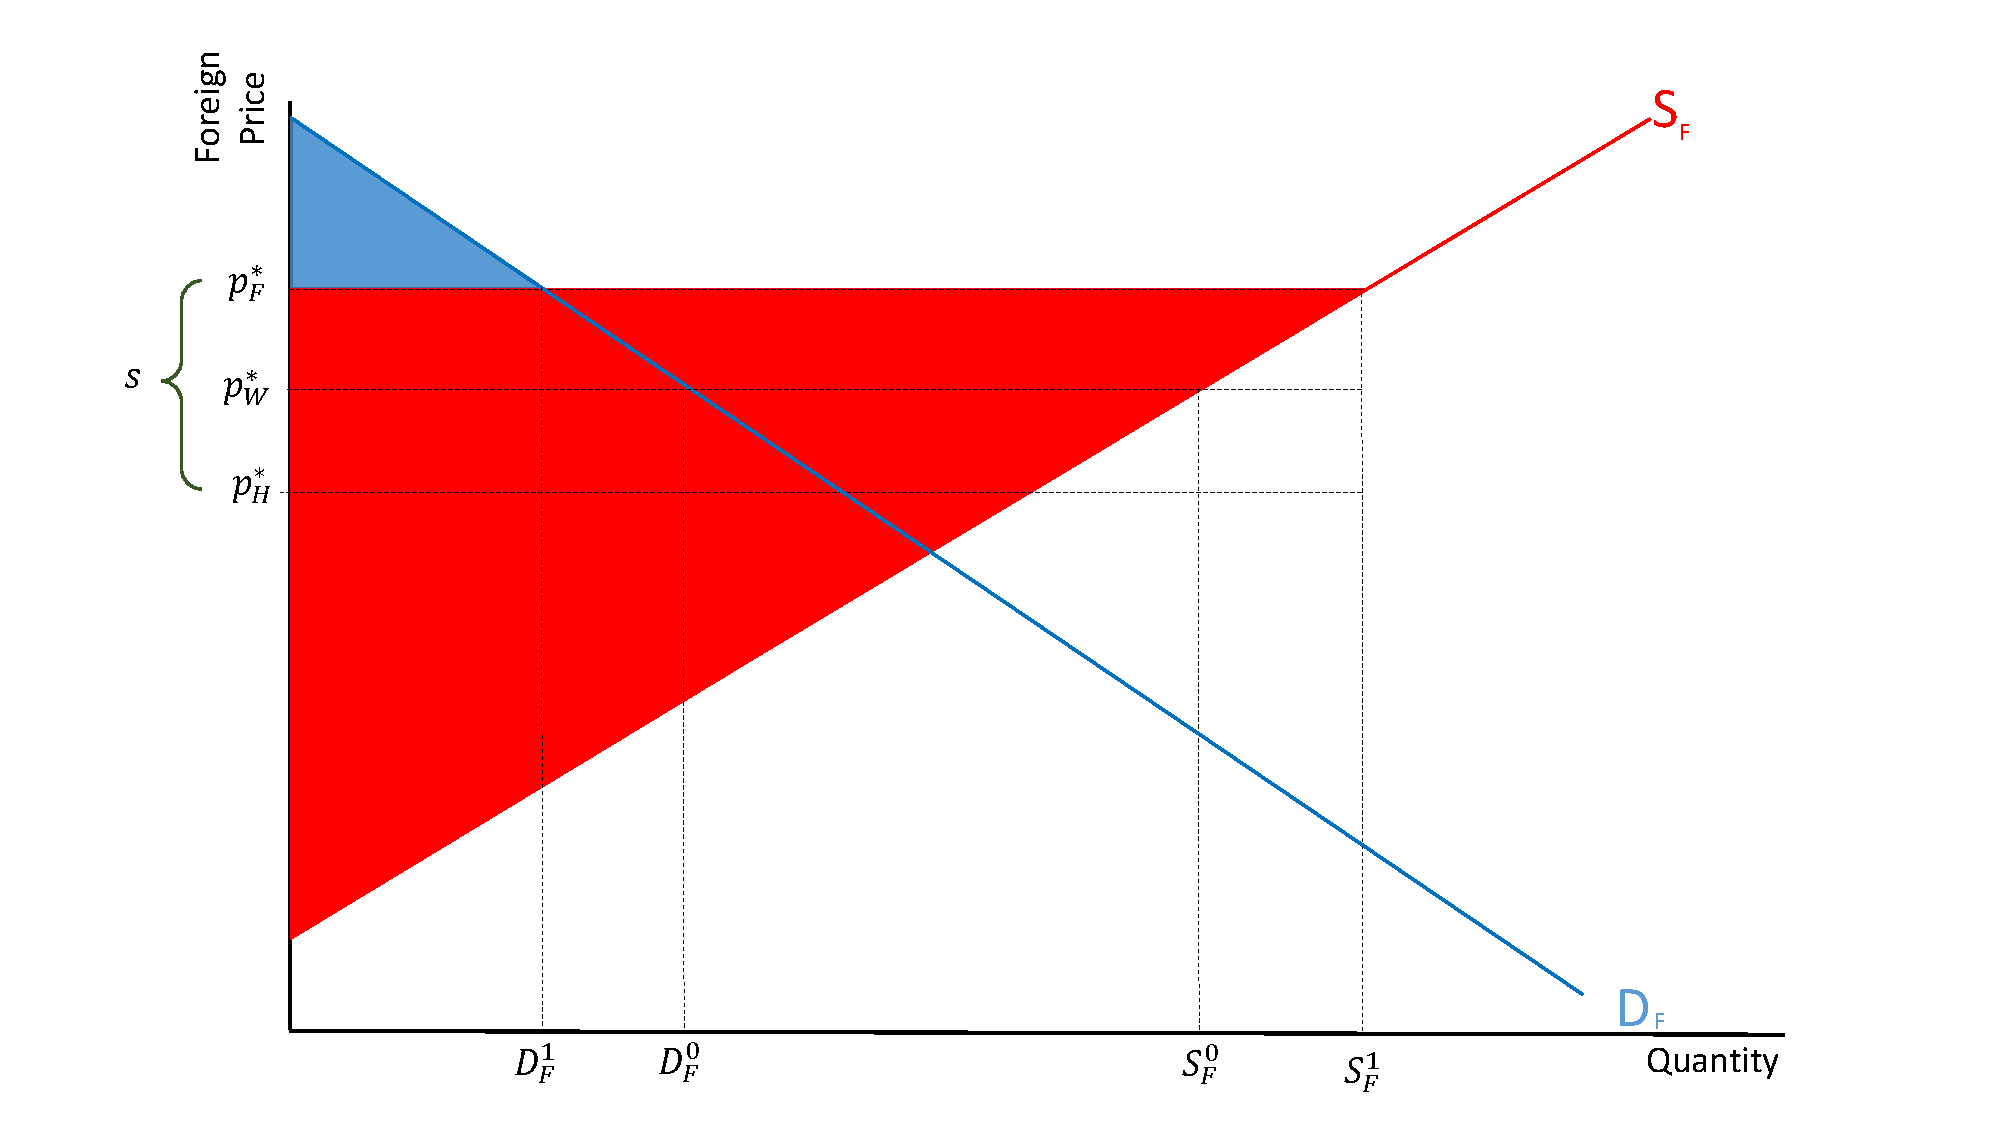
\includegraphics[scale=0.3]{SL_25.pdf}
	
	
	...However, recall that the subsidy must be paid by someone!
	
\end{frame}

\begin{frame}
	\frametitle{Export Subsidies and Foreign Welfare:  Cost of subsidy}
	
	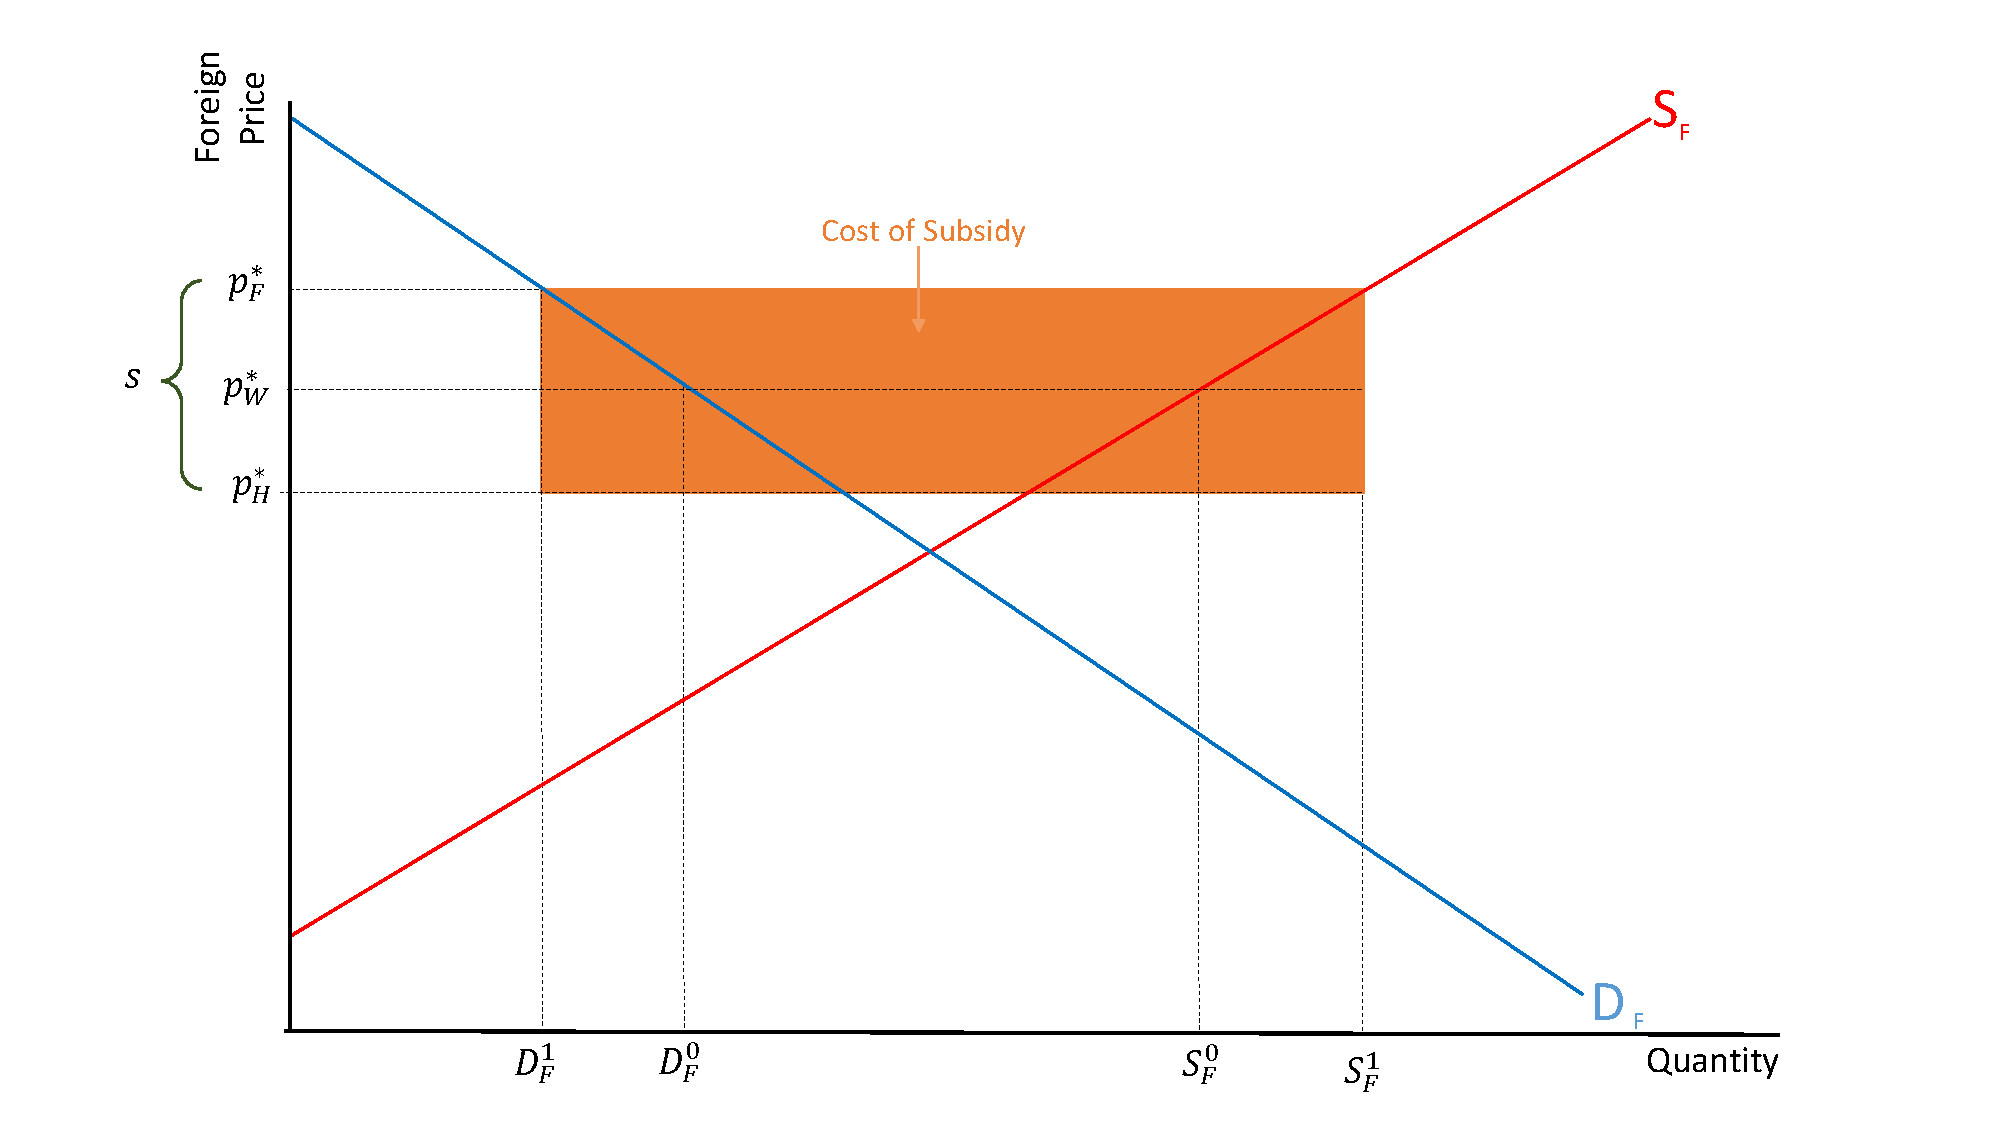
\includegraphics[scale=0.3]{SL_26.pdf}
	
\end{frame}

\begin{frame}
	\frametitle{Export Subsidies and Foreign Welfare:  Change in surplus}
	
	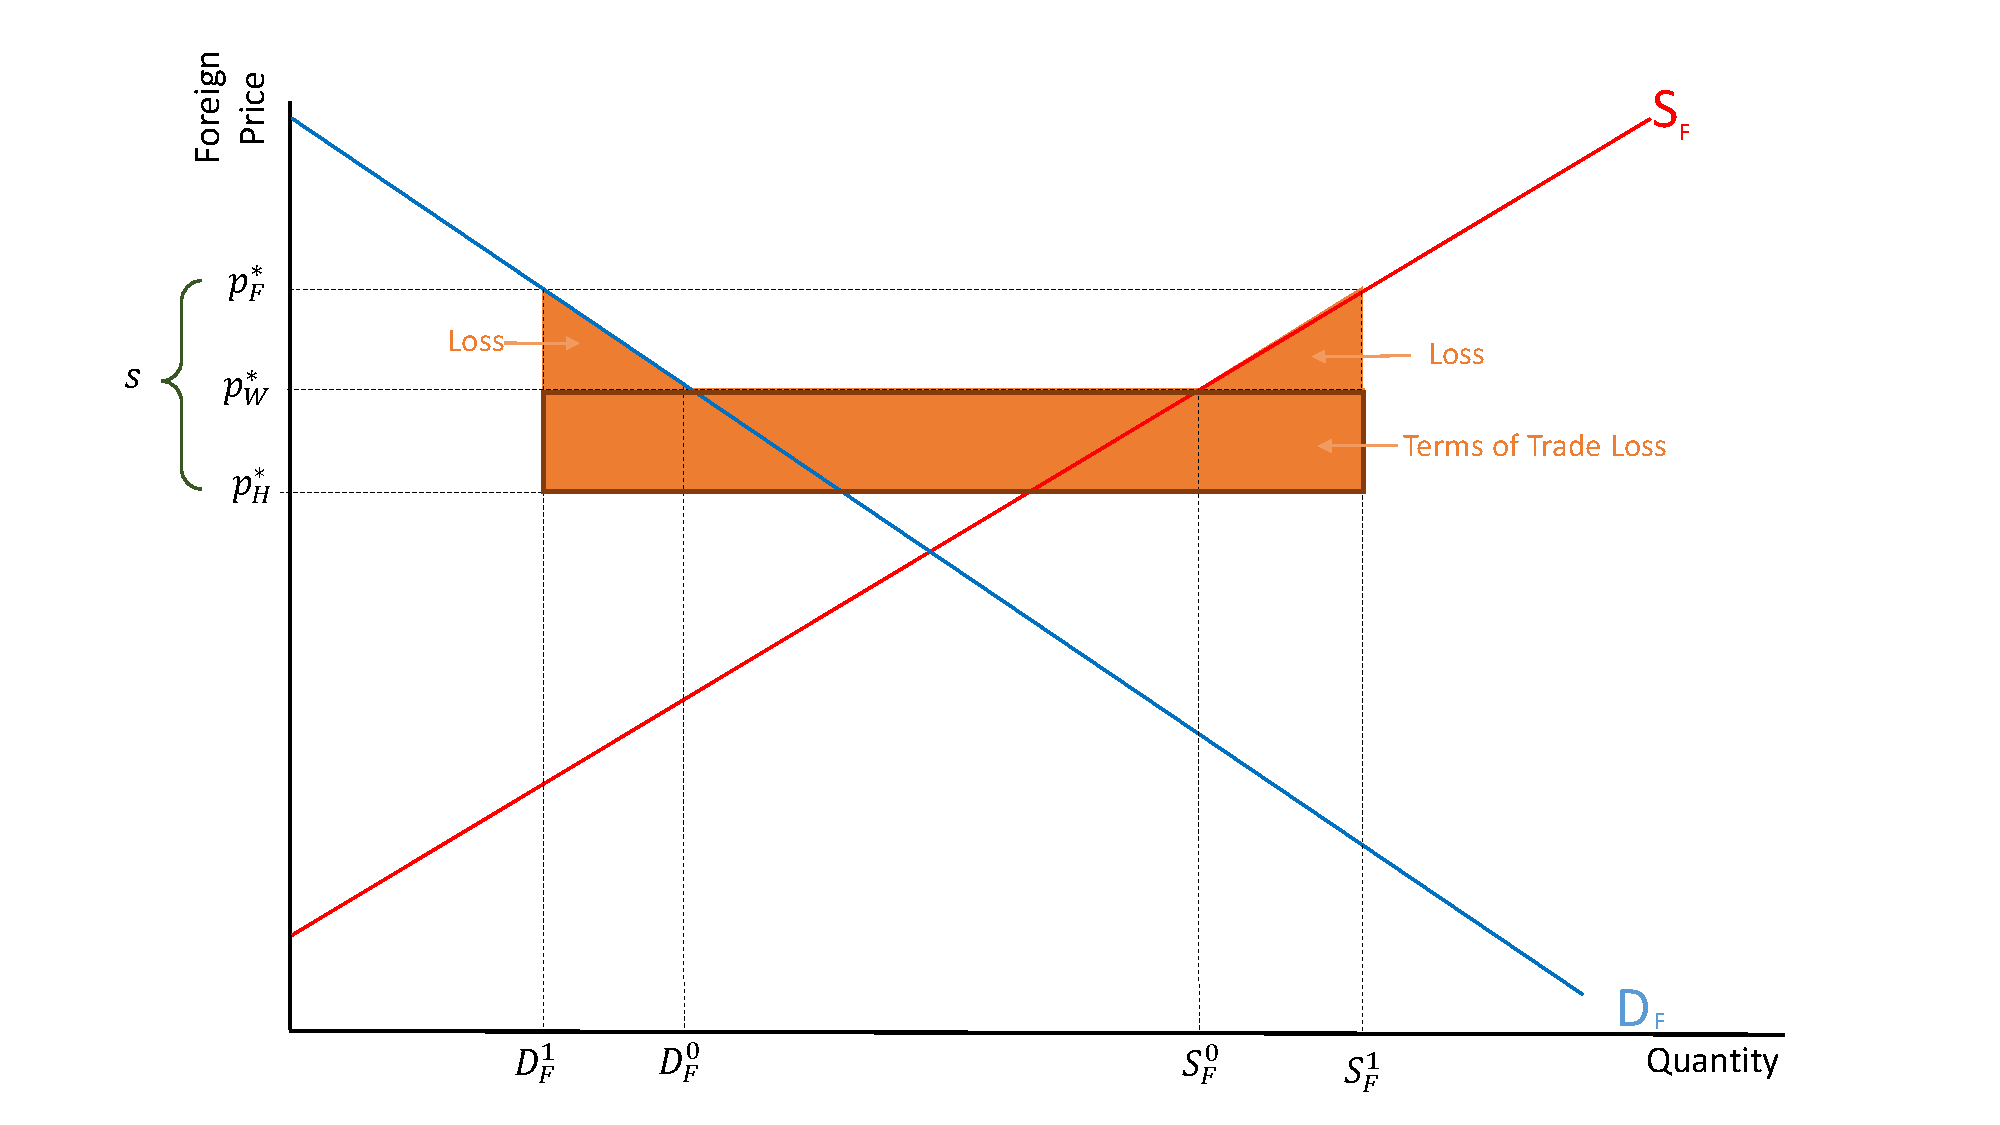
\includegraphics[scale=0.3]{SL_27.pdf}
	
\end{frame}

\begin{frame}
	\frametitle{Export Subsidies:  Summary}
	
	\begin{itemize}
		\item Foreign exports and Home imports rise.
		\item Export subsidies cost the Foreign government money \emph{and decrease} Foreign's terms of trade.
		\begin{itemize}
			\item The Foreign price of the good rises, while the Home price falls.
			\item Leads to an extra welfare cost for the Foreign country.
		\end{itemize}
		\item In general export subsidies do not benefit the exporting country. 
		\begin{itemize}
			\item May be used to achieve distributional goals. 
			\begin{itemize}
				\item Eg. European Common Agricultural Policy.
			\end{itemize} 
		\end{itemize}
		
	\end{itemize}
	
\end{frame}

\subsection{Quotas}
\begin{frame}
	\frametitle{Quotas}
	\textbf{Import Quotas}: A government imposed restriction on the quantity of some good that may imported. 
	\begin{itemize}
		\item Usually enforced issuing import licenses to some limited number of firms.	
		\begin{itemize}
			\item License allows them to import at most some limited quantity of a good. 
		\end{itemize}
		\item Common misconception: Since we are only limiting the quantity of imports, no impact on prices.
		\begin{itemize}
			\item \emph{A (binding) import quota always raises the domestic price of the imported good}
			\begin{itemize}
				\item If import quota binding, then Demand $>$ Supply, domestic prices will be bid up!
			\end{itemize}
		\end{itemize}
	\end{itemize}
	
	
\end{frame}


\begin{frame}
	\frametitle{Quotas: Small Open Economy}
	
	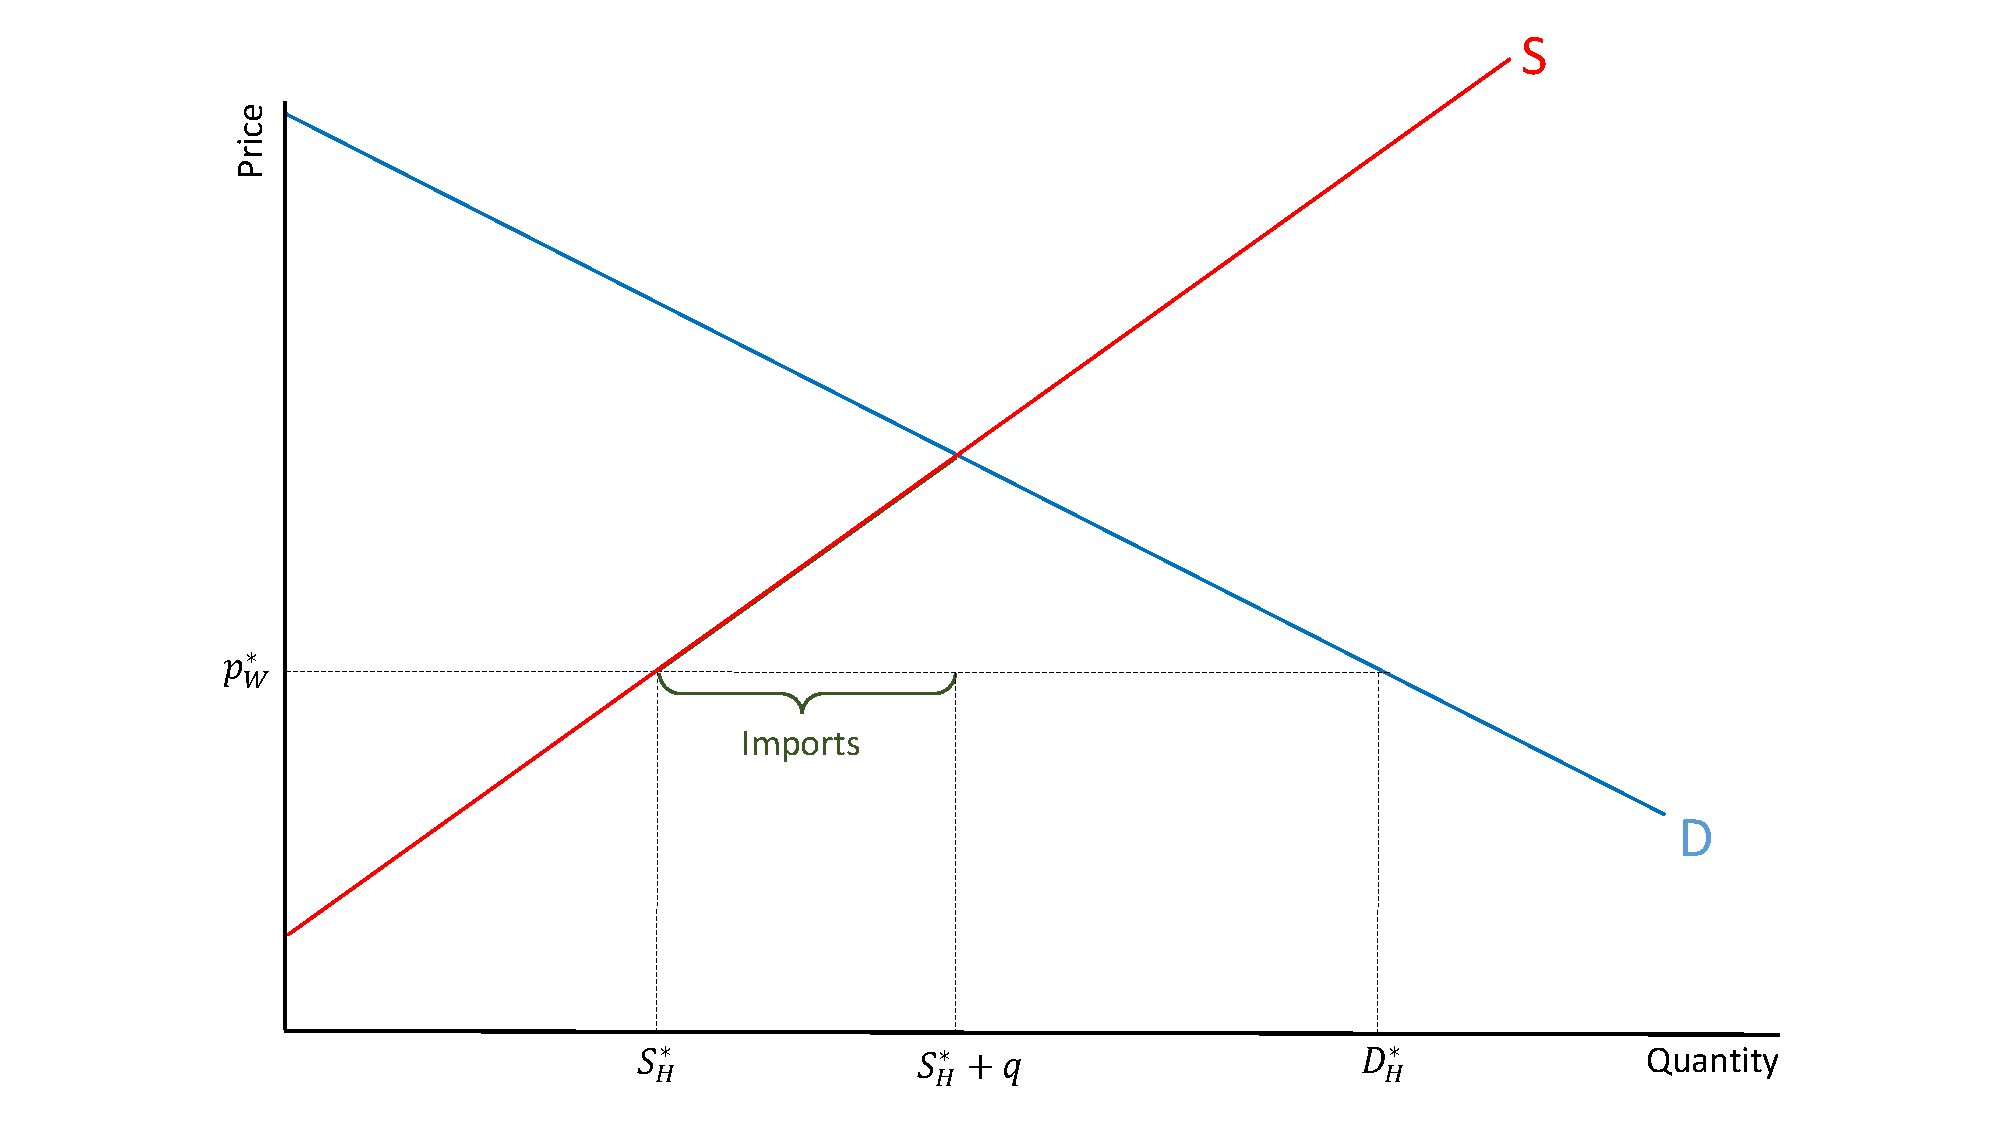
\includegraphics[scale=0.3]{SL_16.pdf}

\end{frame}

\begin{frame}
	\frametitle{Quotas: Small Open Economy}
	
	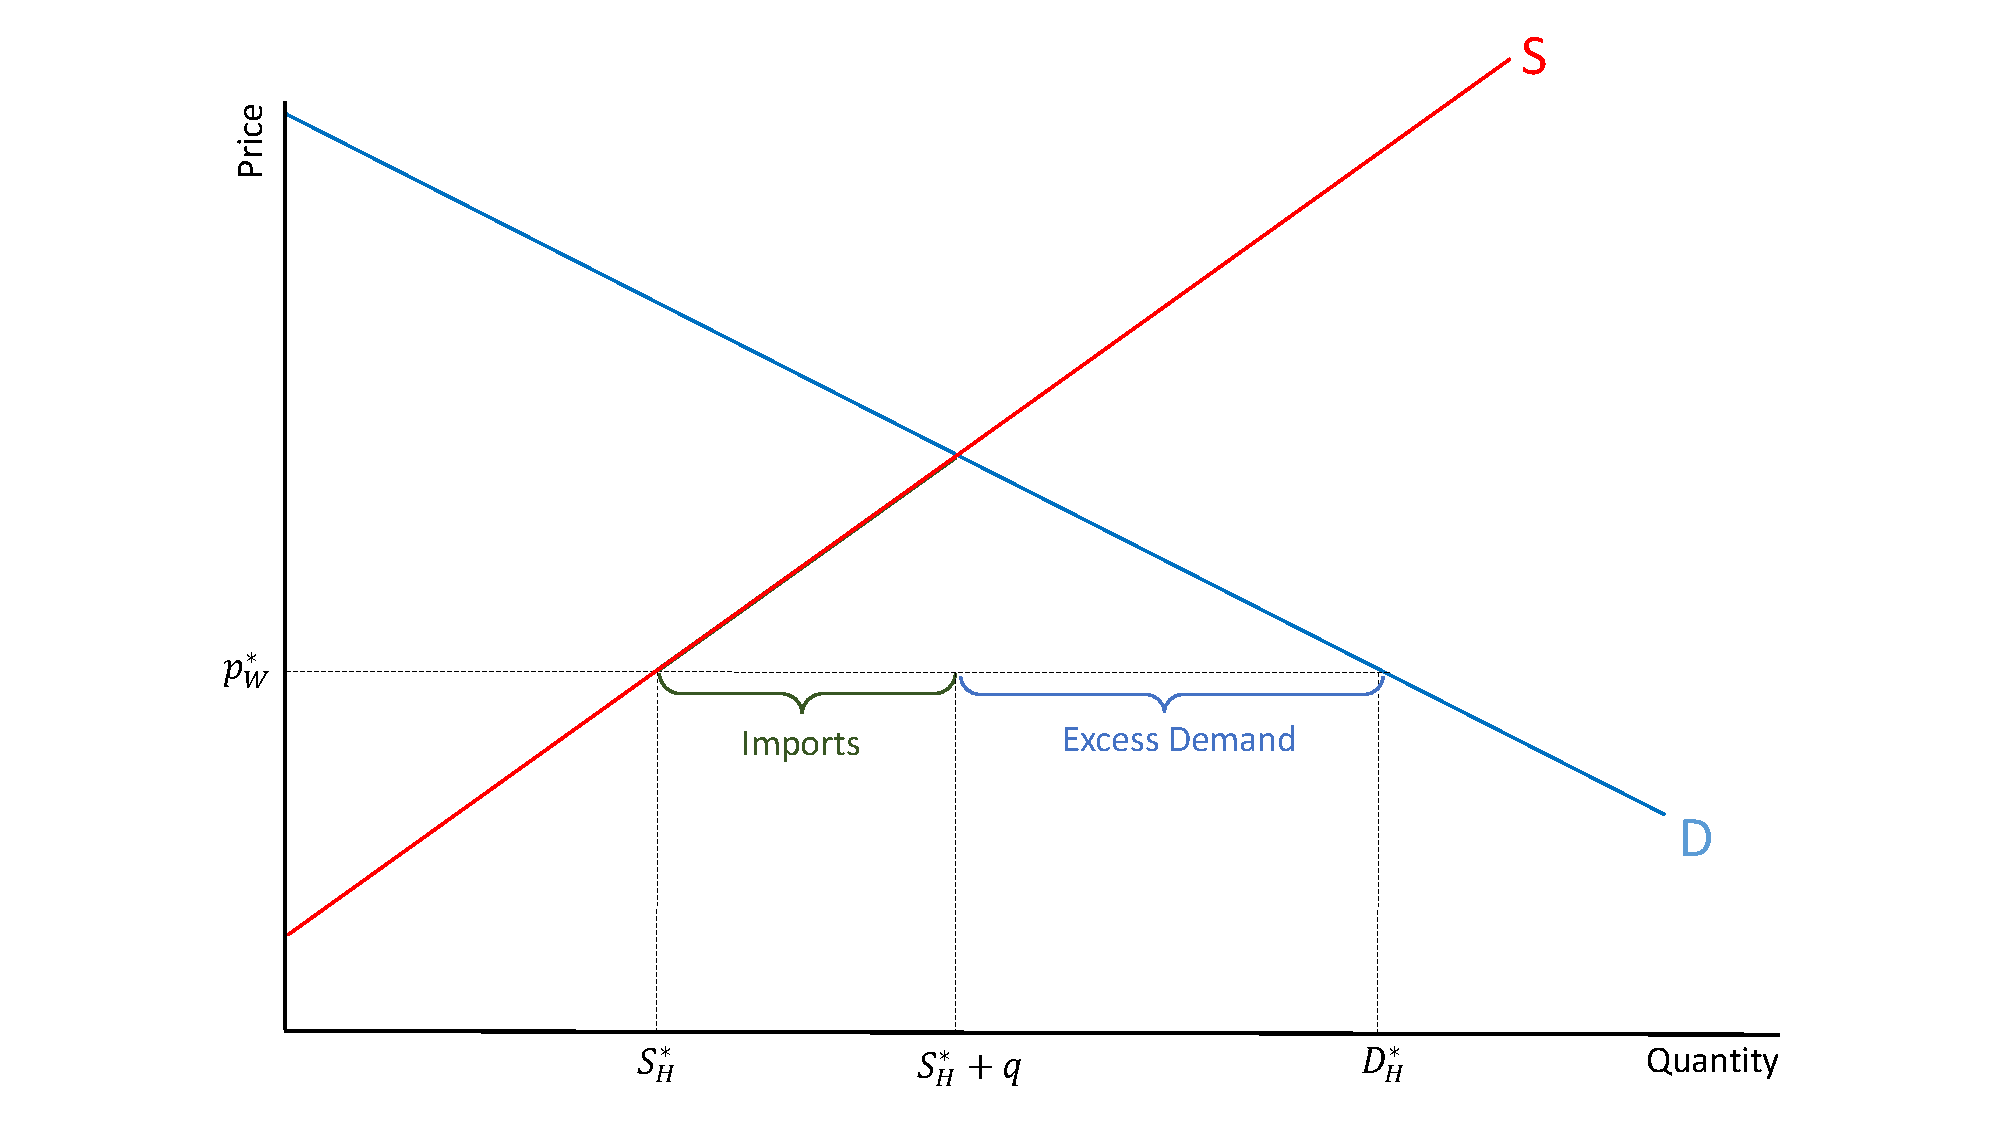
\includegraphics[scale=0.3]{SL_17.pdf}
	
\end{frame}

\begin{frame}
	\frametitle{Quotas: Small Open Economy}
	
	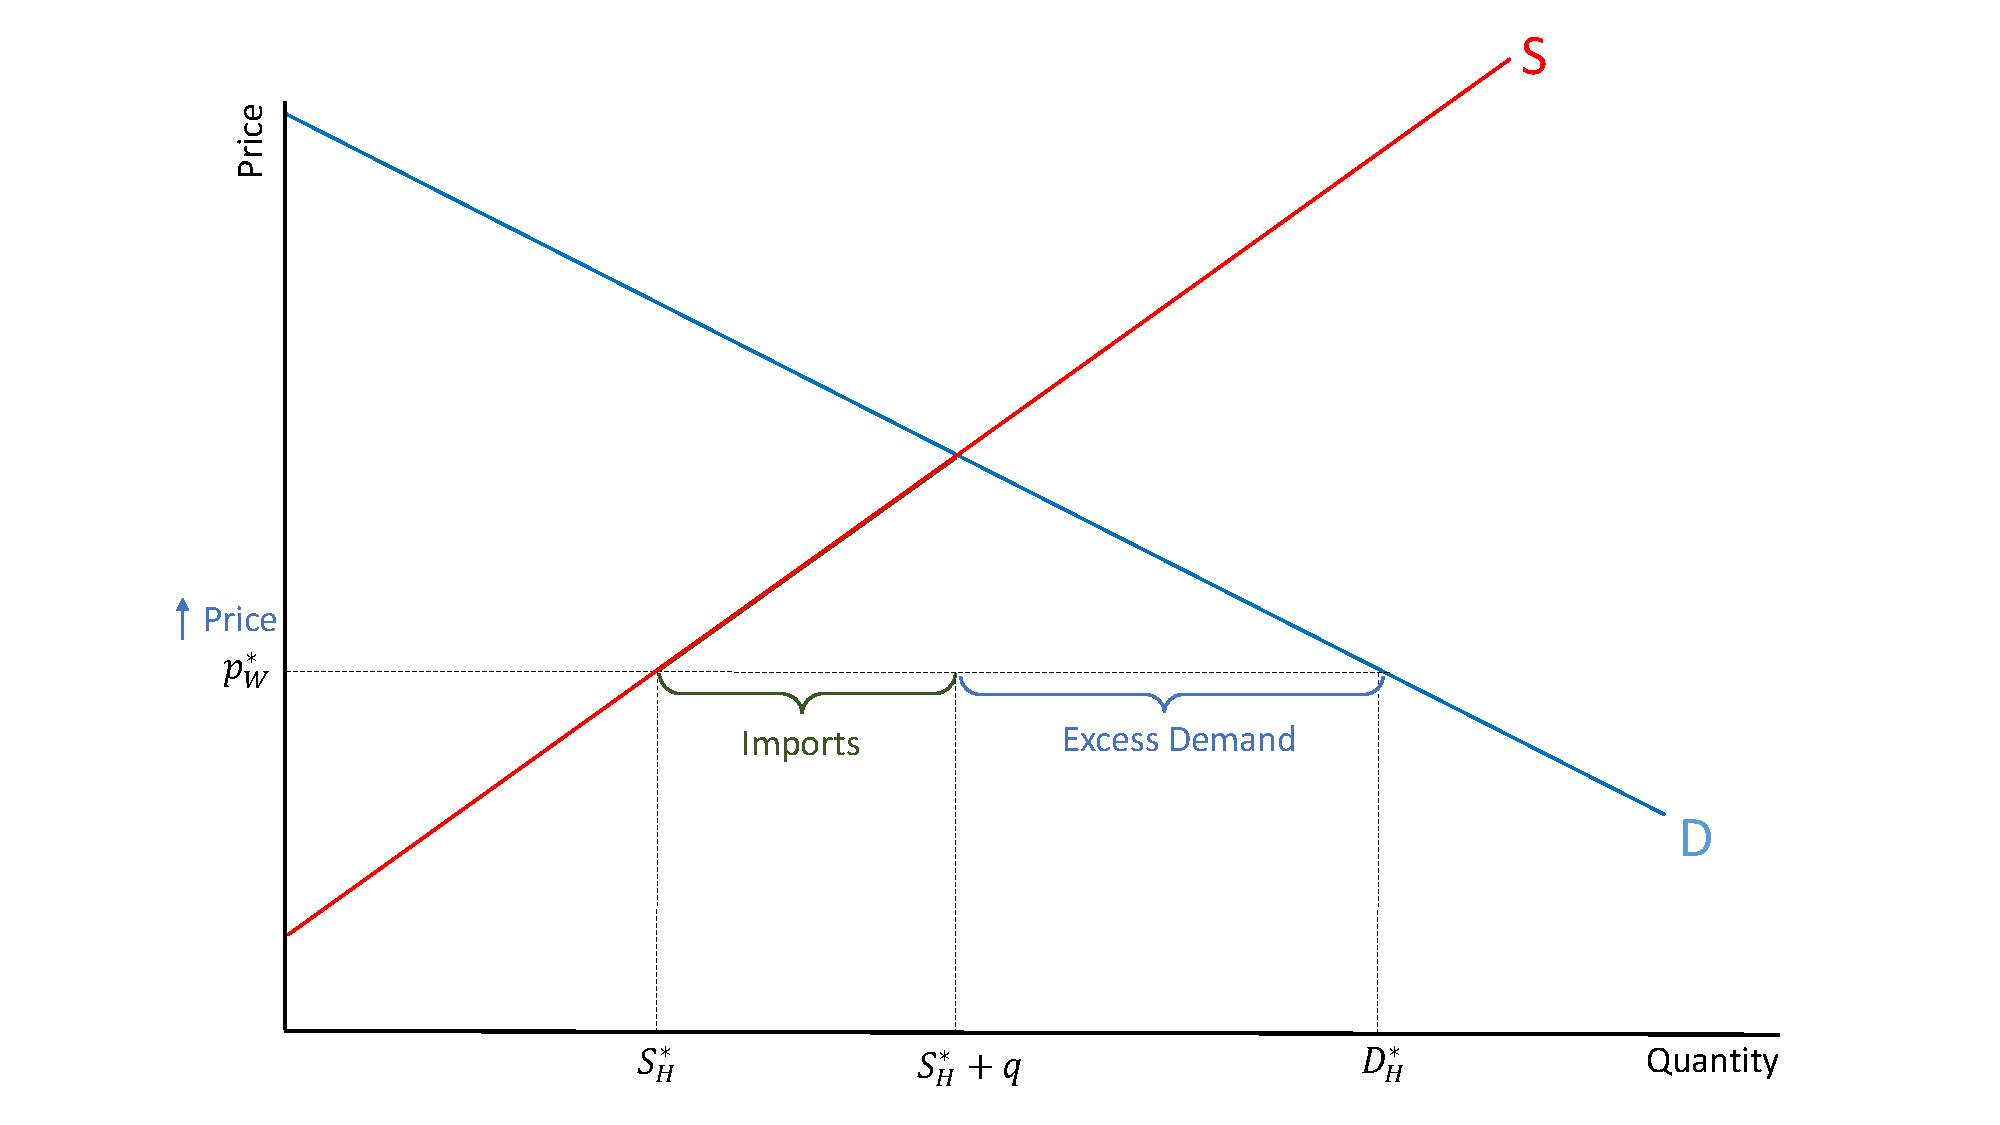
\includegraphics[scale=0.3]{SL_18.pdf}
	
\end{frame}

\begin{frame}
	\frametitle{Quotas: Small Open Economy}
	
	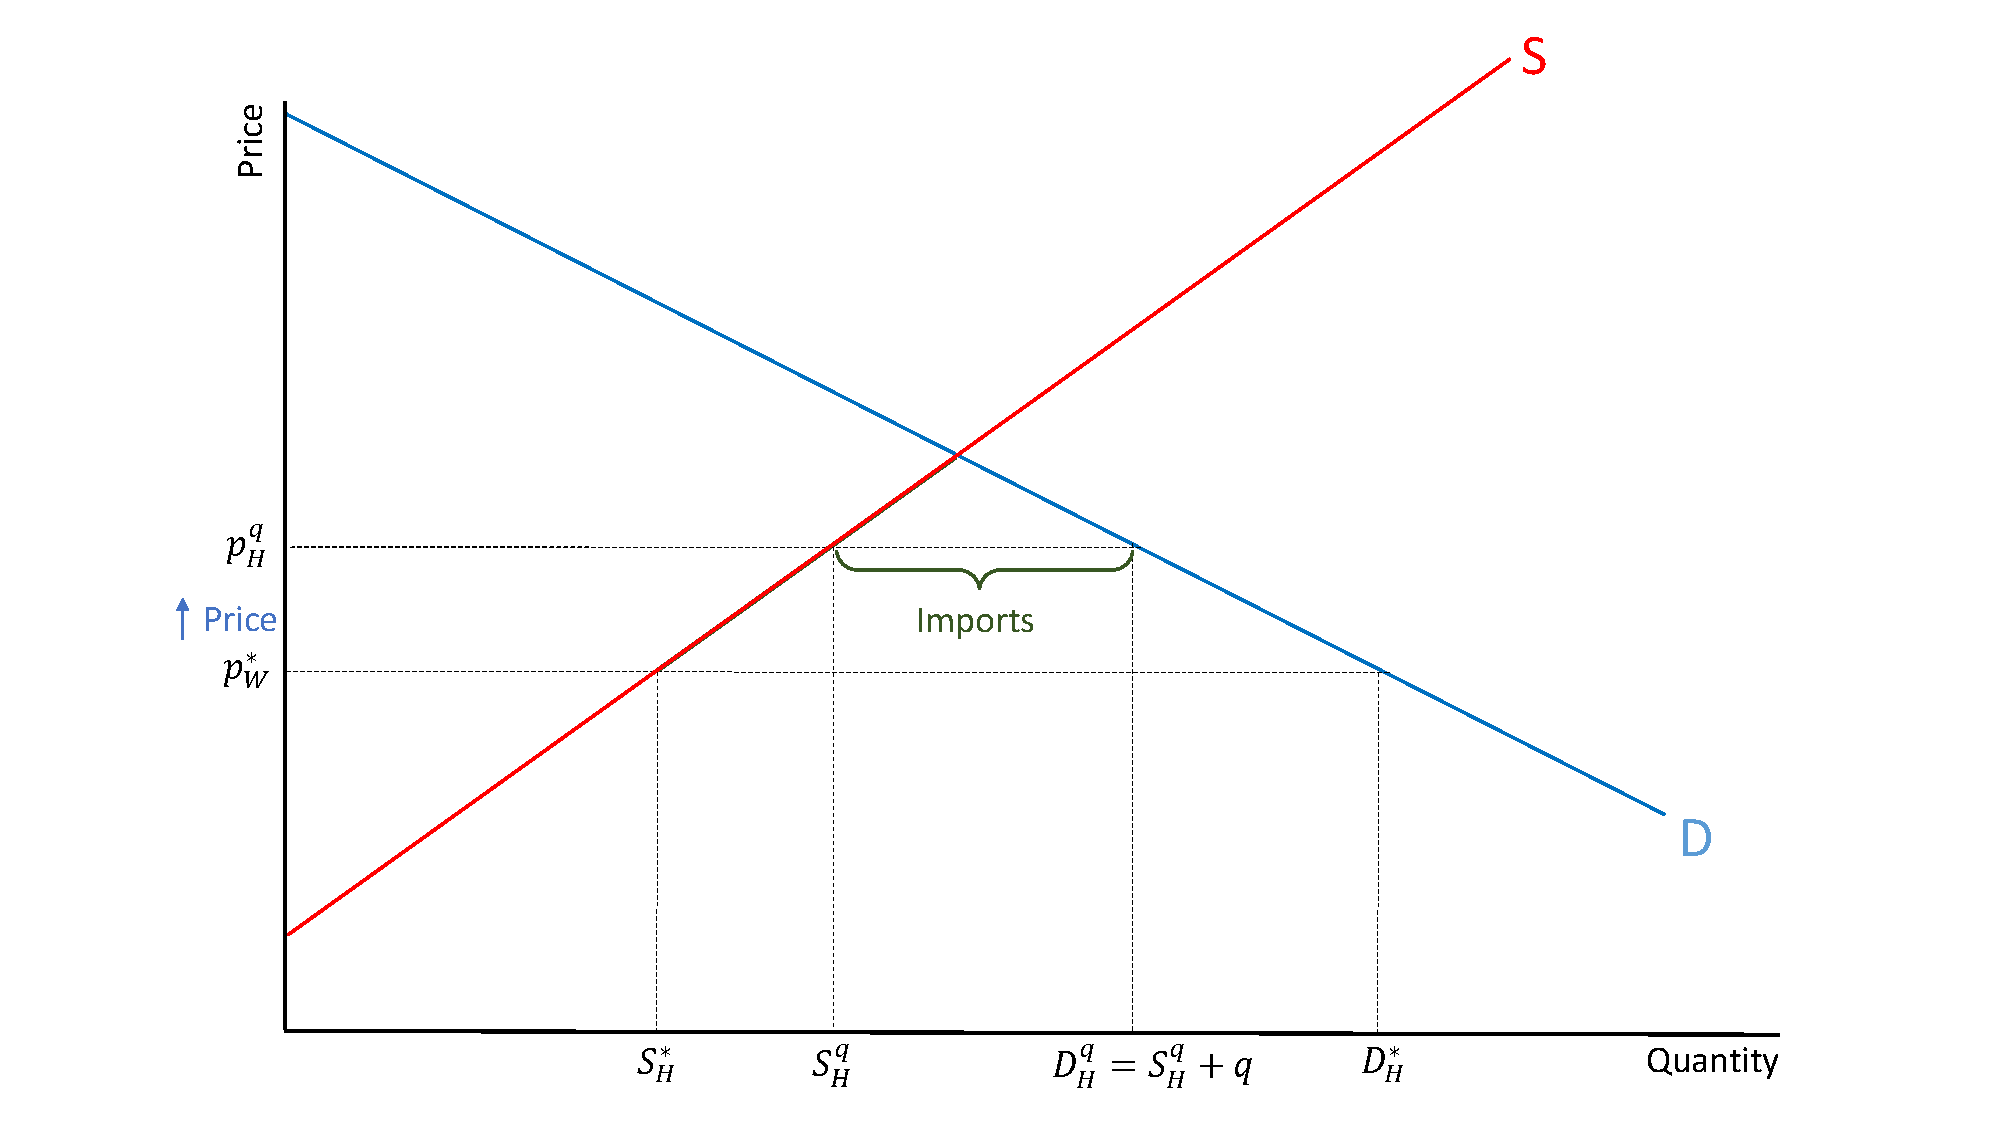
\includegraphics[scale=0.3]{SL_19.pdf}
	
\end{frame}

\begin{frame}
	\frametitle{Quotas and Welfare for SOE: Surplus Pre-Quota}
	
	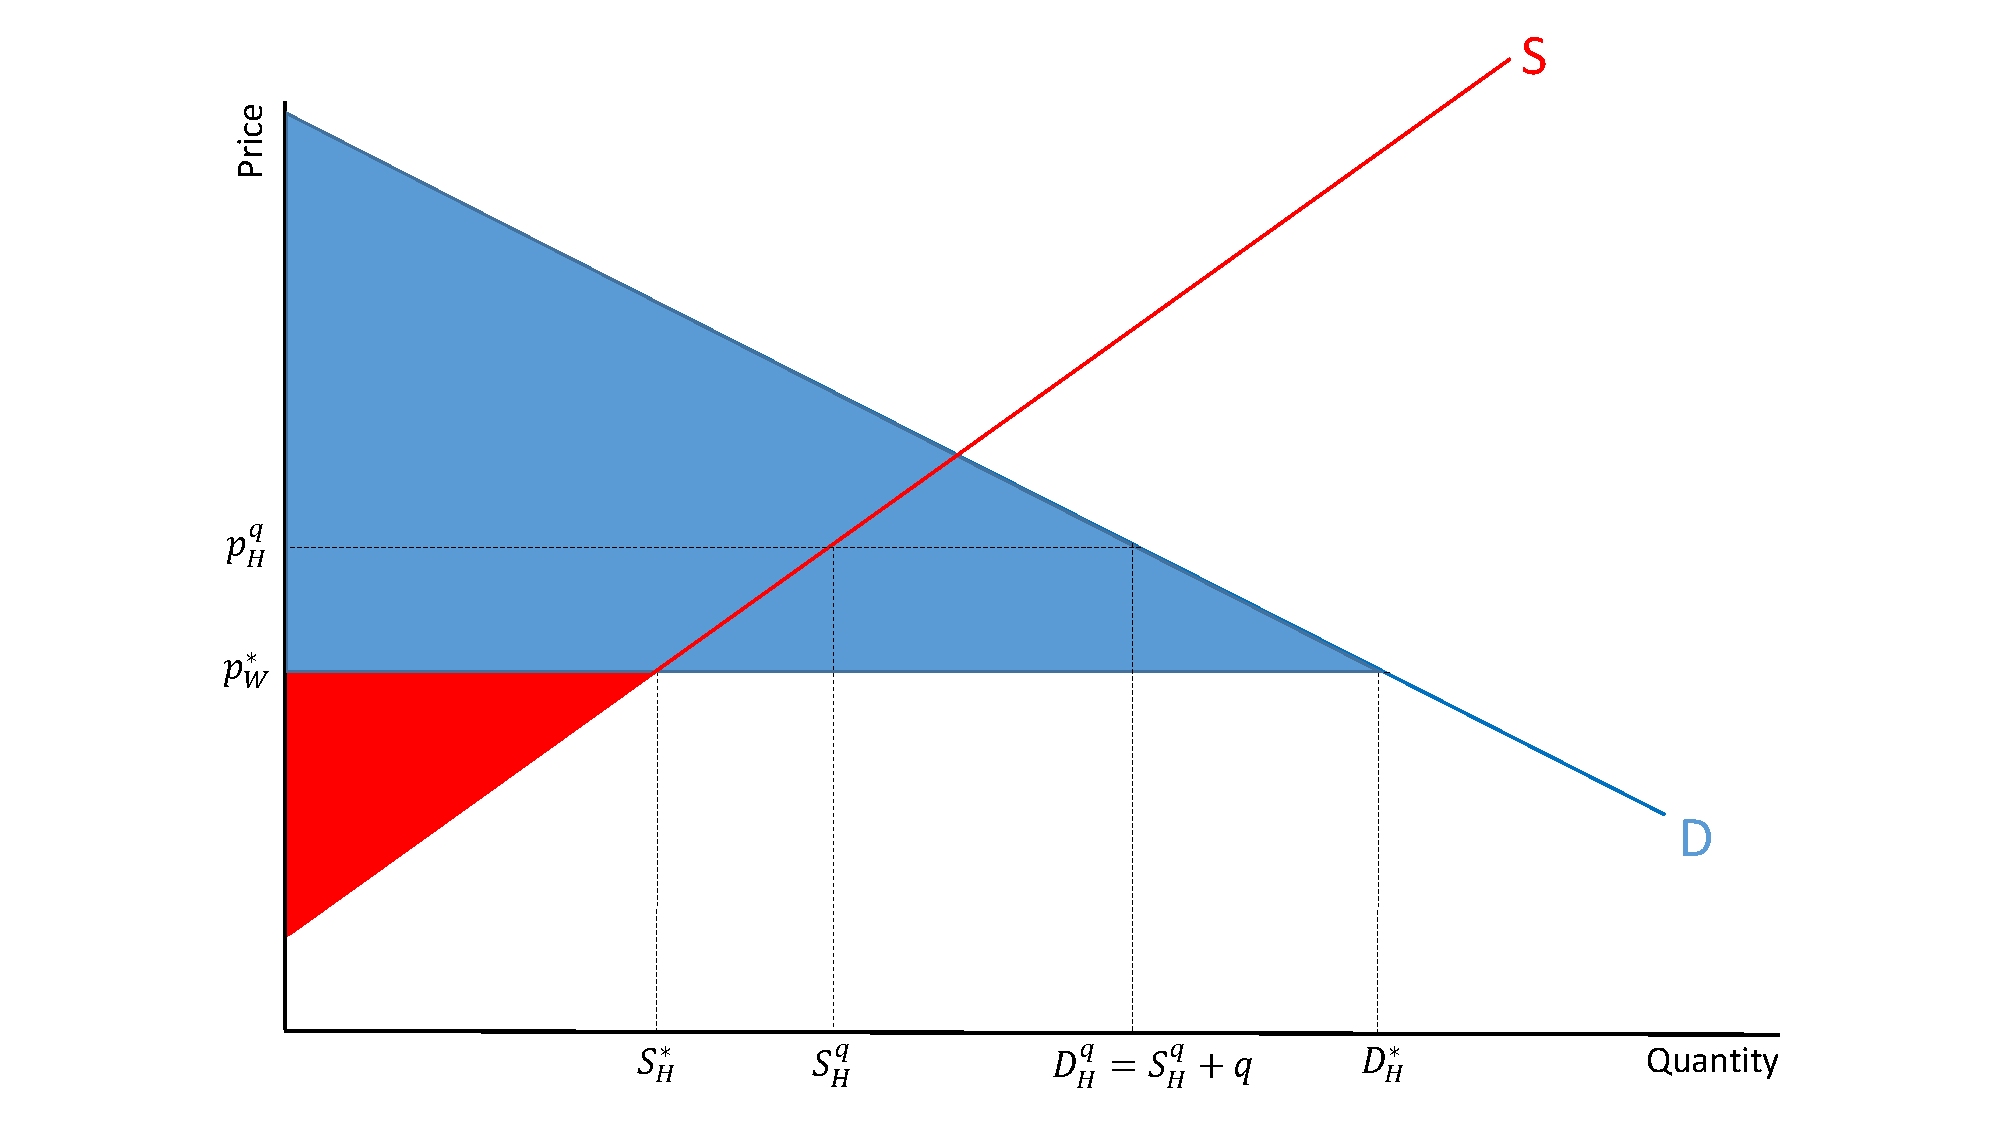
\includegraphics[scale=0.3]{SL_20.pdf}
	
\end{frame}

\begin{frame}
	\frametitle{Quotas and Welfare for SOE: Surplus Post-Quota}
	
	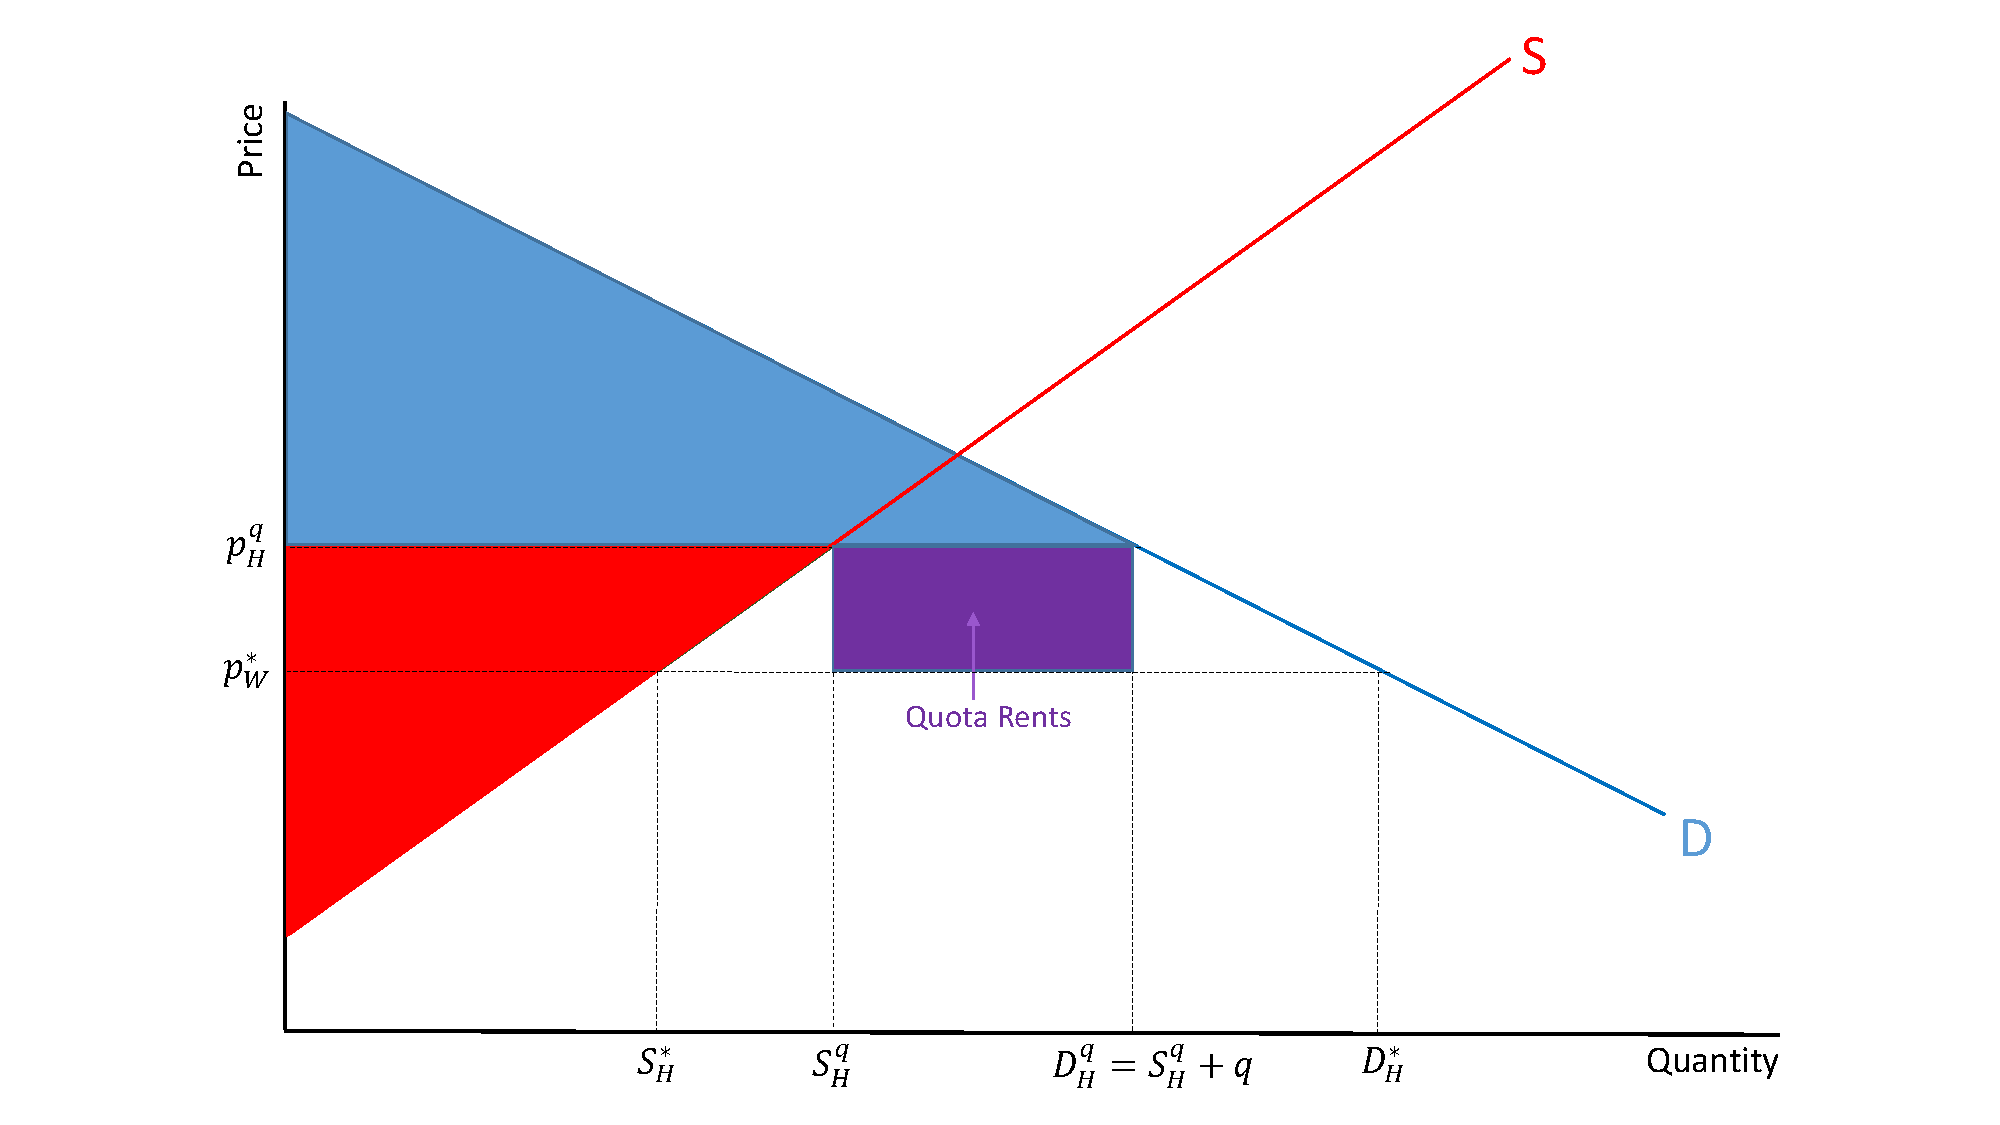
\includegraphics[scale=0.3]{SL_21.pdf}
	
\end{frame}

\begin{frame}
	\frametitle{Quotas and Welfare for SOE: Change in Surplus}
	
	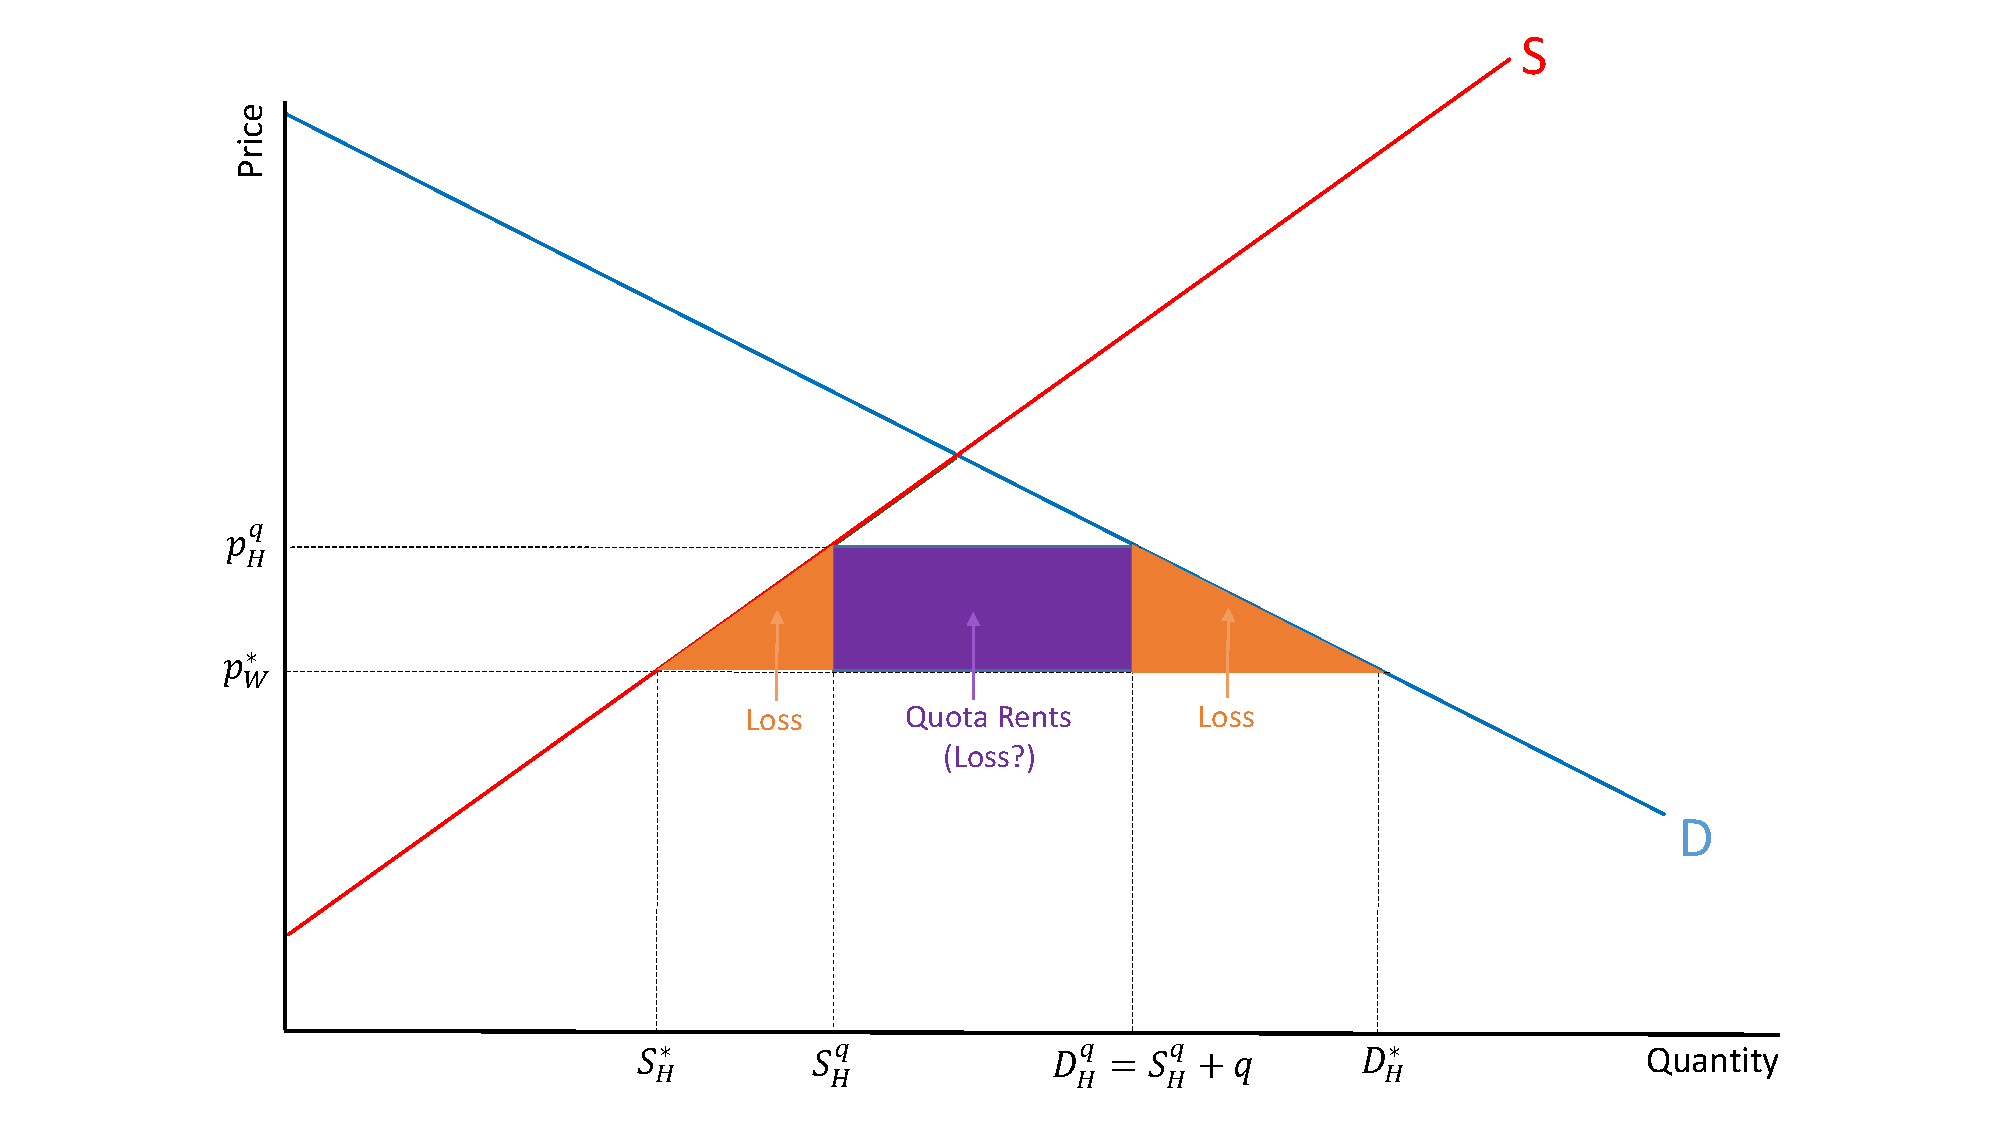
\includegraphics[scale=0.3]{SL_22.pdf}
	
\end{frame}

\begin{frame}
	\frametitle{Summary: Effect of Quotas on SOE}

\begin{itemize}
	\item Imports Fall
	\item Domestic Prices Rise
	\item Welfare Falls
		\begin{itemize}
			\item Welfare falls by less if import licenses given to domestic firms, rather than foreign firms.
		\end{itemize}
\end{itemize}

\begin{center}
What would happen if this was a large open economy? 
\end{center}
	
\end{frame}

\subsection{VERs}

\begin{frame}
	\frametitle{Voluntary Export Restraints (VERs)}
	\begin{itemize}
		\item Essentially a quota imposed on the side of exporting country.
		\item The impact on Home is identical to the quota considered before.
			\begin{itemize}
				\item Except foreign country gets the quota (VER) rents.
				\item Rather than implement a quota, convince exporter to voluntarily restrict trade by giving them some of the rents.
					\begin{itemize}
						\item Less likely to lead to trade war?
						\item Japanese exports of cars to U.S. in 1980s.
					\end{itemize}
			\end{itemize}
	\end{itemize}
	

\end{frame}


\begin{frame}
	\frametitle{Summary}
	\begin{itemize}
		\item Tariffs
		\begin{itemize}
			\item Theory: Small country
				\begin{itemize}
					\item Tariffs tend to hurt small open economies
				\end{itemize}
			\item Theory: Large country
				\begin{itemize}
				\item An optimally chosen tariff will benefit a large country
				\item ... But will hurt other countries (Problem Set 3)
				\end{itemize}
		\end{itemize}
		\item Other Instruments
		\begin{itemize}
			\item Export subsidies
				\begin{itemize}
					\item Hurt large open exporters!
				\end{itemize}
			\item Quotas
				\begin{itemize}
					\item Tends to increase domestic prices, hurts small open economies
				\end{itemize}
			\item Voluntary Export Restraints (VERs)
				\begin{itemize}
					\item A quota imposed by a foreign country.
				\end{itemize}
		\end{itemize}
	\end{itemize}
	
\end{frame}








\begin{comment}


\begin{frame}
\frametitle{How to generate linear demand}
\begin{itemize}
\item Eg: Suppose there are $S$ consumers in this economy, each of whom has (exogenous) income $y$. They wish to allocate their income between food, which costs 1\$ per unit, or (possibly) a car.
\begin{itemize}
\item Each consumer buys at most one car. 
\item All cars are identical, with cost $p$. 
\item Consumers value cars heterogeneously. Let $A_i$ denote the utility consumer $i$ attaches to a car. 
\end{itemize} 
\item Consumer $i$ solves:
\begin{equation}
\max\{A_i + \alpha F;\alpha F\} \qquad \qquad s.t. F + p \leq y 
\end{equation}
\end{itemize}
\end{frame}




\newpage


\noindent  \emph{Total surplus} is the sum of producer and consumer surplus. Note that: \\

\begin{itemize}
  \item Surpluses can be added.
  \item This ignores distributional issues.
 \begin{itemize}
 \item Is this reasonable?
 \end{itemize}
\end{itemize}

\newpage

\begin{center}
\textbf{Analysis of a Tariff in a Large Country}
\end{center}

\noindent Consider two countries, Home and Foreign, and a good that (i) is produced competitively and (ii) traded costlessly. Assume that \emph{Home} imports the good from \emph{Foreign}.

\noindent Two new concepts needed:
\begin{itemize}
  \item Import demand
  \item Export supply
  \item Note: With two goods, \emph{Home} will export the other good under balanced trade.
\end{itemize}

\noindent \emph{Import demand} measures for each price, the excess of what Home consumers demand over what Home producers supply.

\newpage

\begin{center}
Deriving the Import Demand Curve
\end{center}

\begin{figure}
  \begin{center}
\resizebox{!}{5in}{\includegraphics{slide93}}
  \end{center}
\end{figure}

\newpage

\noindent Properties of the import demand curve:
\begin{itemize}
  \item It intersects the vertical axis at the closed economy price of the
  importing country.
  \item It is downward sloping.
\end{itemize}

\noindent\emph{Export supply} measures for each price, the excess of what Foreign producers supply over what Foreign consumers demand.

\newpage

\begin{center}
Deriving the Export Supply Curve
\end{center}

\begin{figure}
  \begin{center}
\resizebox{!}{5in}{\includegraphics{slide94}}
  \end{center}
\end{figure}

\newpage

\noindent Properties of the export supply curve:
\begin{itemize}
\item It intersects the vertical axis at the closed economy price of the exporting country.
\item It is upward sloping.
\end{itemize}

\newpage

\begin{center}
Definitions
\end{center}
\begin{itemize}
\item Assume that for a given good, home pays price $p^{H}$ and foreign pays price $p^{F}$.
\item Assume that the ``world price", $p^{W}$, is the price without tariffs.
\begin{itemize}
\item Without tariffs, $p^{H}=p^{F}=p^{W}$.
\end{itemize}
\item Define a \textbf{large} country as one that can affect the world price level.
\item Define a \textbf{small} country as one that cannot affect the world price level.
\end{itemize}

\newpage

\noindent Effect of a tariff in a Large Country.
\begin{figure}
  \begin{center}
\resizebox{!}{5in}{\includegraphics{slide95}}
  \end{center}
\end{figure}

\newpage

\begin{itemize}
  \item Under free trade, prices are equalized across countries.
  \item With a tariff, the price in Home rises from $P^W$ to $P^{H}$
  \begin{itemize}
    \item Home producers supply more and consumers demand less.
  \item Home imports decline
  \end{itemize}
  \item With a tariff, the price in Foreign decreases.
\begin{itemize}
  \item Foreign producers supply less and consumers demand more.
    \item Foreign exports decline
  \end{itemize}
  \item The increase in $p^{H}$ is less than the tariff, because part of the tariff is reflected in a decline in $p^{F}$.
\end{itemize}

\newpage

\begin{itemize}
\item Solving for prices and trade under free trade:
\begin{enumerate}
\item Calculate autarky free trade prices for each country. The country with the lower autarky price will be the exporter of that good.\\
\item Set excess/export  supply for the exporter ($S^{*}(p^{W})-D^{*}(p^{W})$) equal to excess/import demand for the importer ($D(p^{W})-S(p^{W})$). \\
\item Solve for $p^{W}$. \\
\begin{itemize}
\item This is the world free trade equilibrium price.\\
\end{itemize}
\item Substitute equilibrium world prices back into the export supply and import demand functions to solve for equilibrium trade.\\
\end{enumerate}
\end{itemize}

\newpage

\begin{itemize}
\item Solving for prices and trade with tariffs:
\begin{enumerate}
\item Define $p^{F}$ as the price that foreign suppliers receive.\\
\item The home price will be $p^{F}+\tau$ where $\tau$ is the specific tariff.\\
\item Set excess/export  supply for the exporter ($S^{*}(p^{F})-D^{*}(p^{F})$) equal to excess/import demand for the importer ($D(p^{F}+\tau)-S(p^{F}+\tau)$). \\
\item Solve for $p^{F}$.\\
\begin{itemize}
\item $p^{F}$ will be the world price that foreign exporters receive. \\
\item $p^{H}=p^{F}+\tau$ will be the home price.\\
\end{itemize}
\end{enumerate}
\item What are the welfare effects of such a tariff?
\end{itemize}

\newpage

\begin{center}
Free Trade (importing country's point of view)
\end{center}

\begin{figure}
  \begin{center}
\resizebox{!}{4.5in}{\includegraphics{slide96}}
  \end{center}
\end{figure}

\newpage

\begin{figure}
  \begin{center}
\resizebox{!}{5in}{\includegraphics{slide97}}
  \end{center}
\end{figure}

\newpage


\noindent Ambiguous net welfare effect of Tariffs in a large country.

\begin{figure}
  \begin{center}
\resizebox{!}{5in}{\includegraphics{slide98}}
  \end{center}
\end{figure}

\newpage

\begin{figure}
  \begin{center}
\resizebox{!}{5in}{\includegraphics{slide99}}
  \end{center}
\end{figure}

\newpage

\begin{center}
Interpretation
\end{center}
\noindent Following a tariff:

\begin{itemize}
  \item Producer surplus increases (a)
  \item Consumers surplus decreases (a+b+c+d)
  \item Government surplus arises (c+e)
  \item total change in surplus (e-b-d)
\end{itemize}

\newpage

\noindent A tariff in a large country:
\begin{itemize}
\item has its incidence born \emph{jointly} by both the home and foreign countries,
  \item raises the price of the good in the importing country,
  \begin{itemize}
     \item consumers lose in that country
     \item producers gain in that country
  \end{itemize}
  \item creates tariff revenue in the importing country,
  \begin{itemize}
  \item Assume that tariff revenue is returned to the population.
  \end{itemize}
  \item lowers the price of the good in the exporting country.
  \begin{itemize}
     \item Consumers gain in that country
     \item Producers lose in that country
  \end{itemize}
\end{itemize}

\newpage

\noindent Overall in the importing country:
\begin{itemize}
  \item deadweight loss,
  \item term of trade gain,
  \item overall net effect is ambiguous.
  \begin{itemize}
  \item Depends on the slope of the export supply curve for Foreign. The tariff may benefit the importing country if the terms of trade effect is strong enough with a very steep export supply curve.
  \end{itemize}
\end{itemize}

\newpage

\noindent Overall in the exporting country:
\begin{itemize}
  \item producers lose,
  \item consumers gain,
  \item overall welfare falls for the foreign country.
\end{itemize}

\newpage

\begin{center}
Optimal Tariffs Under Perfect Competition for a Large Country
\end{center}

\begin{itemize}
\item An ``optimal" tariff maximizes the terms of trade gain net of the deadweight loss.
\item We can derive the deadweight loss areas and the terms of trade gain in terms of model parameters.
\item With equations for demand and supply for Home and Foreign countries, we can calculate the optimal tariff.\\
\end{itemize}

\newpage

\begin{figure}
  \begin{center}
\resizebox{!}{5in}{\includegraphics{slide99}}
  \end{center}
\end{figure}

\newpage

\begin{itemize}
\item Export supply curve for the exporting country: $EX\left(P^{F}\right)=g+hP^{F}$
\item Import demand curve for the importing country
\begin{itemize}
\item $D\left(P^{H}\right)=a-dP^{H}$ \   \   \ $S\left(P^{H}\right)=c+eP^{H}$
\item $IM\left(P^{H}\right)=D(P^{H})-S(P^{H})=(a-c)-(d+e)P^{H}$
\item $IM\left(P^{H}\right)=b-fP^{H}$
\end{itemize}
\item World Price without tariffs
\begin{itemize}
\item $P^{W}=\frac{b-g}{f+h}$.
\end{itemize}
\item Prices with tariffs
\begin{itemize}
\item $P^{F}=P^{W}-\tau\frac{f}{f+h}=\frac{b-g-f\tau}{f+h}$
\item $P^{H}=P^{W}+\tau\frac{h}{f+h}=\frac{b-g+h\tau}{f+h}$.
\end{itemize}
\end{itemize}

\newpage
\begin{center}
Incidence of a Tariff imposed by a large economy
\end{center}
\begin{itemize}
\item $P^{F}=P^{W}-\tau\frac{f}{f+h}$
\item $P^{H}=P^{W}+\tau\frac{h}{f+h}$.
\item As imports demand becomes more elastic ($f\uparrow$), the exporter bears a higher incidence of the tariff. 
\item As export supply becomes more elastic ($h\uparrow$), the importer bears a higher incidence of the tariff.
\end{itemize}
\newpage

\begin{itemize}
\item Area $e$ equals $IM\left(P^{H}\right)\left(P^{W}-P^{F}\right)$.
\item Area $b$ equals $\frac{1}{2}e\left(P^{H}-P^{W}\right)^{2}$.
\item Area $d$ equals $\frac{1}{2}d\left(P^{H}-P^{W}\right)^{2}$.

\begin{center}
\begin{large}
$e-b-d$=$\left[b-f\left[\frac{b-g+h\tau}{f+h}\right]\right]\frac{f\tau}{f+h}-\frac{(e+d)h^{2}\tau^{2}}{2(f+h)^{2}}$.
\end{large}
\end{center}
\newpage
\item The net gain from the tariff will look like $tU-t^{2}V$ where $U$ and $V$ are functions of the constants above. Consequently, it will be quadratic, and the optimal tariff is where the slope and derivative are equal to zero.
\item $\tau^{*}=\frac{U}{2V}=\frac{bfh+gf^{2}}{2hf^{2}+(e+d)h^{2}}$
\item Note: This is solved out explicitly in the appendix to Ch. 9 and appears on the tariffs practice problems.
\item Notice that the optimal tariff for the importing country is falling in the elasticity of export supply ($h$).
\end{itemize}

\newpage

\begin{figure}
  \begin{center}
\resizebox{!}{5in}{\includegraphics{slide107}}
  \end{center}
\end{figure}

\begin{center}
Analysis of a tariff in small country
\end{center}

\begin{figure}
  \begin{center}
\resizebox{!}{5in}{\includegraphics{slide100}}
  \end{center}
\end{figure}


\newpage

\noindent Equilibrium with a tariff

\begin{figure}
  \begin{center}
\resizebox{!}{5in}{\includegraphics{slide101}}
  \end{center}
\end{figure}

\newpage

\noindent Welfare gain/loss with a tariff

\begin{figure}
  \begin{center}
\resizebox{!}{5in}{\includegraphics{slide102}}
  \end{center}
\end{figure}


\newpage

\begin{itemize}
\item Because the world price is now fixed, home consumers absorb the entire incidence of the tariff.
\item Deadweight loss no longer offset by terms of trade appreciation.
\item Small countries (by definition) cannot affect world prices.
\item Welfare loss.
\item Optimal tariff for a small country is $0\%$.
\end{itemize}

\newpage



\begin{center}
The Effective Rate of Protection
\end{center}

\begin{itemize}
\item Suppose now that we are talking about an \emph{ad valorem} (percentage) tariff.
\item How much protection does a tariff provide? 
\item Problem 1:
\begin{itemize}
\item Usually thought of as the difference in the price in a country with the tariff versus that price in the same country without the tariff.
\item For a large country, this will only capture the amount that the home price rises and not the amount that the foreign price falls $\left(P^{H}-P{W}=\frac{th}{f+h}<t\right)$.
\end{itemize}
 \newpage
  \item Problem 2: Intermediate goods and the difference between output and value added.
  \begin{itemize}
  \item This will be a problem for both small and large countries.
  \item key insight: tariffs are imposed on the entire value of the good, not just the value added in the good.
  \end{itemize}
\item Let's focus on problem 2.
\item Define the \textbf{effective protection rate}
\begin{center}
$f=\left(\frac{V_{T}-V_{W}}{V_{W}}\right)100$.
\end{center}
\item Define $V_{T}$ and $V_{W}$ as value added with and without the tariff, respectively. 
\end{itemize}

\newpage

\begin{itemize}
\item Imagine a Canadian car sold \$20,000 in Canada (a ``small" country). This car contains \$15,000 worth of intermediate inputs from the U.S.
\item Canada imposes a 25\% tariff on car imports from the \textsc{US} that raises the price of cars in Canada to \$25,000.
\item What rate of protection do Canadian car producers really receive?


\item Effective protection rate:$\left(\frac{(25,000-15,000)-(20,000-15,000)}{20,000-15,000}\right)100=100\%>25\%$.


\end{itemize}

\newpage

\begin{itemize}
\item For another example of the second problem, Canada places a 20\% tariff on car intermediate inputs from the \textsc{us}.\\
\begin{itemize}
\item Canadian intermediate input providers benefit.
\item What is Canada's protection for \emph{car producers}?\\
\item Assume that the price of cars is fixed based on world markets.\\
\item  A tariff of $20\%$ on components raises their price to \$18,000.\\
\item $(\frac{(20,000-18,000)-(20,000-15,000)}{20,000-15,000})100=-60\%<0\%$.\\
\end{itemize}
\end{itemize}

\newpage
\begin{center}
\item Real life example: U.S. steel protection in 2002.
\end{center}
\begin{itemize}
\item In 2002, George W. Bush imposed 8\%-30\% steel tariffs.
\item Large and important ``Rust Belt" swing states of Pennsylvania and West Virginia would benefit from the tariffs. 
\item The tariffs would harm consumers and U.S. businesses that relied on steel imports, and would cost more jobs in industries that relied on steel than it would save in steel industries.
\item Tariffs lifted in 2003.
\end{itemize}

\newpage

\newpage
 
\noindent Ad-valorem tariff has similar effects as specific tariffs.

\begin{center}
\includegraphics[scale=0.6]{Tariff_1}
\end{center}

\newpage

\begin{figure*}
\begin{center}
\caption{Effects of an Export Subsidy in a large country}
\includegraphics[scale=0.7]{Tariff_2}
\end{center}
\end{figure*}

\newpage

\begin{itemize}
\item An \textbf{export subsidy} is a payment to a firm or individual that ships a good abroad.
\item It raises prices in the exporting country while lowering them in the importing country.
\item Producer gain (a+b+c)
\item Consumer loss (a+b)
\item Cost of government subsidy (b+c+d+e+f+g)
\item Net welfare loss (b+d+e+f+g)
\item In contrast to a tariff, the export subsidy \emph{worsens} the terms of trade (e+f+g)
\end{itemize}

\newpage

\begin{figure*}
\begin{center}
\caption{Effect of an Import Quota in a small country}
\includegraphics[scale=0.7]{Tariff_3}
\end{center}
\end{figure*}

\newpage

\begin{itemize}
\item An \textbf{import quota} is a direct restriction on the quantity of some good that may be imported.
\item It \emph{always raises the domestic price of the imported good}.
\item The difference between a quota and a tariff is that with a quota, the government receives no revenue. 
\item  The sum of money that would have appeared with a tariff as government revenue is collected by whoever receives at the import license.
\item Consumer loss (a+b+c+d)
\item Producer gain (a)
\item Quota rents (c)
\end{itemize}

\newpage

\begin{itemize}
\item A variant on the import quota is the \textbf{voluntary export restraint (VER)}
\item A VER is a quota on trade imposed from the exporting country's side instead of the importer's.
\item The most famous example is the limitation on auto exports to the U.S. enforced by Japan after 1981.
\item Certain political and legal advantages have made VERs preferred instruments of trade policy in some cases.
\item From en economics point of view, however, a VER is exactly like an import quota.
\item What would have been revenue under a tariff becomes rents earned by foreigners under the VER.\
\end{itemize}


%-=-=-=-=-=-=-=-=-=-=-=-=-=-=-=-=-=-=-=-=-=-=-=-=-=-=-=-=-=-=-=-=-=-=-=-=
\foilhead[-.7in]{Trade and Politics}
%-=-=-=-=-=-=-=-=-=-=-=-=-=-=-=-=-=-=-=-=-=-=-=-=-=-=-=-=-=-=-=-=-=-=-=-=

\begin{itemize}
\item In this topic, we try to examine the reasons why governments should not, or do not base their trade policy on economists cost-benefit calculations.
\item Objectives and Agenda
\begin{itemize}
\item The cases for free trade\\
\item The cases against free trade\\
\item The political economy of trade
\begin{itemize}
\item collective action problems,
\item who lobbies for protection in each industry\\
\end{itemize}
\item Trade institutions (e.g. The World Trade Organization (WTO)).
\end{itemize}
\end{itemize}

%-=-=-=-=-=-=-=-=-=-=-=-=-=-=-=-=-=-=-=-=-=-=-=-=-=-=-=-=-=-=-=-=-=-=-=-=
\foilhead[-.7in]{\small{The Case for Free Trade 1: Free Trade and Efficiency}}
%-=-=-=-=-=-=-=-=-=-=-=-=-=-=-=-=-=-=-=-=-=-=-=-=-=-=-=-=-=-=-=-=-=-=-=-=

\begin{itemize}
\item A tariff causes a net loss to the economy measured by the area of the two triangles:
\end{itemize}

\begin{figure*}
\begin{center}
\includegraphics[scale=0.5]{Tariff_4}
\end{center}
\end{figure*}

\newpage

\begin{itemize}
\item Is it important quantitatively?
\item In the modern world, tariff rates are generally low and import quotas relatively rare.
\item As a result, estimates of the total costs of distortions due to tarisdds and import quotas tend to me modest in size.
\item For most countries, the gains from further trade liberalization may be small ($1\%$ \textsc{gdp}?)
\end{itemize}

\begin{table*}
\caption{\textbf{Benefits of a Move to Worldwide Free Trade}}
\vspace{0.5in}
\begin{center}
\begin{tabular}{c c c }
Country & & Gain (\% of GDP) \\
\hline
United States & &  0.57 \\
European Union & &   0.61 \\
Japan & &   0.85\\
Developing Countries & &   1.4\\
World & &   0.93\\
\hline
\multicolumn{3}{c}{Source: Cline (2004) as in Krugman and Obstfeld.}
\end{tabular}
\end{center}
\label{default}
\end{table*}%

\begin{itemize}
\item Larger or smaller numbers can be derived with more elaborate models but the general magnitudes and patterns are generally robust.
\end{itemize}


%-=-=-=-=-=-=-=-=-=-=-=-=-=-=-=-=-=-=-=-=-=-=-=-=-=-=-=-=-=-=-=-=-=-=-=-=-=-=-=-=-=-=-=-=
\foilhead[-.7in]{\small{The Case for Free Trade 2: Additional Gains from Free Trade}}
%-=-=-=-=-=-=-=-=-=-=-=-=-=-=-=-=-=-=-=-=-=-=-=-=-=-=-=-=-=-=-=-=-=-=-=-=-=-=-=-=-=-=-=-=

\begin{itemize}
\item Better exploitation of internal and existing external economies of scale.
\item Competition with imports incentivizes learning and innovation.
\item Cleansing effect of export selection improves the efficiency of the economy as a whole.
\end{itemize}

%-=-=-=-=-=-=-=-=-=-=-=-=-=-=-=-=-=-=-=-=-=-=-=-=-=-=-=-=-=-=-=-=-=-=-=-=
\foilhead[-.7in]{\small{The Case for Free Trade 3: Rent-seeking}}
%-=-=-=-=-=-=-=-=-=-=-=-=-=-=-=-=-=-=-=-=-=-=-=-=-=-=-=-=-=-=-=-=-=-=-=-=

\begin{itemize}
\item When imports are restricted with a quota rather than a tariff, the cost is sometimes magnified by a process known as \textbf{rent-seeking}.
\item To enforce a quota, the government has to issue import licenses. In some cases, individuals and companies incur substantial costs in an effort to get import licenses. 
\item To conclude, even though there might be better policies than free trade, they may always end up being manipulated by special interests
\item It may be better to promote free trade without exceptions.
\end{itemize}

\newpage
 
%-=-=-=-=-=-=-=-=-=-=-=-=-=-=-=-=-=-=-=-=-=-=-=-=-=-=-=-=-=-=-=-=-=-=-=-=
\foilhead[-.7in]{National Welfare Argument Against Free Trade}
%-=-=-=-=-=-=-=-=-=-=-=-=-=-=-=-=-=-=-=-=-=-=-=-=-=-=-=-=-=-=-=-=-=-=-=-=

\begin{itemize}
\item Most tariffs, import quotas, and other trade policy measures are undertaken primarily to protect the income of particular interest groups.
\item Although they are often claimed to be undertaken in the interest of the nation as a whole.
\item Although economists often argue against deviations from free trade, there are some theoretical grounds for believing that activist trade policies can sometimes increase the welfare of the nation as a whole:
\begin{enumerate}
\item The terms of trade argument
\item The domestic market failure argument
\item The strategic trade policy argument 
\end{enumerate}
\end{itemize}

%-=-=-=-=-=-=-=-=-=-=-=-=-=-=-=-=-=-=-=-=-=-=-=-=-=-=-=-=-=-=-=-=-=-=-=-=
\foilhead[-.7in]{The Terms of Trade Argument Against Free Trade}
%-=-=-=-=-=-=-=-=-=-=-=-=-=-=-=-=-=-=-=-=-=-=-=-=-=-=-=-=-=-=-=-=-=-=-=-=

\begin{itemize}
\item Optimal tariff (on both the import and export sectors)
\item Important limitations:
  \begin{itemize}
  \item For small countries, they have little power to affect the world price of either their imports or exports. 
  \item For large countries, such predatory policy might result in retaliation.
  \item Generally not seen in relevant policy discussions.
  \item Tariffs tend to be higher in developing countries.
  \end{itemize}
\end{itemize}

%-=-=-=-=-=-=-=-=-=-=-=-=-=-=-=-=-=-=-=-=-=-=-=-=-=-=-=-=-=-=-=-=-=-=-=-=
\foilhead[-.7in]{The Domestic Market Failure Argument Against Free Trade}
%-=-=-=-=-=-=-=-=-=-=-=-=-=-=-=-=-=-=-=-=-=-=-=-=-=-=-=-=-=-=-=-=-=-=-=-=

\begin{itemize}
\item The labor market and capital market may not be as well-functioning as the theory assumes (domestic market failure).
\item To mitigate the short run costs of these malfunctioning market, trade policy may be a good instrument.
\item For example, labor market inefficiency makes it difficult for unemployed workers to find a new job. Then trade policy protecting the import-competing industry seems like a good idea, at least in the short run. 
\item In this sense, rather than a cost, trade is less of a cause of the protectionist policy, but rather a "second-best" alternative.
\end{itemize}

%-=-=-=-=-=-=-=-=-=-=-=-=-=-=-=-=-=-=-=-=-=-=-=-=-=-=-=-=-=-=-=-=-=-=-=-=
\foilhead[-.7in]{Strategic Trade Policy Argument Against Free Trade}
%-=-=-=-=-=-=-=-=-=-=-=-=-=-=-=-=-=-=-=-=-=-=-=-=-=-=-=-=-=-=-=-=-=-=-=-=

\begin{itemize}
\item Strategic trade policy\\
\begin{itemize}
\item With a foreign monopoly, the home government can use trade policy to capture some of the monopoly rents.\\
\item Under imperfect competition with both home and foreign producers, trade policy can be used to shift profits to the home firm.\\
\end{itemize}

\newpage

\item Infant industry\\
\begin{itemize}
\item A country may have a comparative advantage but cannot initially compete with established industries in other countries.\\
\item To foster their development, governments can temporarily support them until they have grown strong enough.\\
\end{itemize}
\item Objections:
\begin{itemize}
\item The short-run cost of protection may outweigh the long-run gain even if the policy is successful.
\item In addition, ``temporary" protection is often renegotiated. 
\item Protection may not foster productivity growth
\item Why does the government need to become involved?
\end{itemize}
\end{itemize}

\newpage

\begin{center}
Overall
\end{center}

\noindent A good case for free trade, but why does it meet so much resistance?\\[3ex]
\noindent Difficult question
\begin{itemize}
\item Trade issues are very badly understood
\item Trade policies are determined by the political process
\begin{itemize}
\item Those who are harmed by trade tend to be very concentrated.
\item Those who benefit from trade tend to be very diffuse.
\end{itemize}
 \end{itemize}
 
 
%-=-=-=-=-=-=-=-=-=-=-=-=-=-=-=-=-=-=-=-=-=-=-=-=-=-=-=-=-=-=-=-=-=-=-=-=
\foilhead[-.7in]{Trade and politics: Collective Action Problem}
%-=-=-=-=-=-=-=-=-=-=-=-=-=-=-=-=-=-=-=-=-=-=-=-=-=-=-=-=-=-=-=-=-=-=-=-=

\begin{itemize}
\item Why do small groups who are hurt by a policy lobby so hard against the policy and large groups who benefit from it so unlikely to lobby for it?
\item Suppose that each consumer gains relatively little from trade.
\item With many consumers though, the aggregate gains can be large.
\item Despite the large aggregate gains, each individual expends very little effort lobbying for free trade.
\end{itemize}

\newpage

\begin{itemize}
\item Losers from trade are often hurt dramatically from import competition.
\begin{itemize}
\item Ontario and Michigan auto makes.
\item Quebec and European diary farmers.
\end{itemize}
\item However, there are relatively few of them.
\item Aggregate losses are small but these are the agents who end up doing all of the lobbying.
\item Heckscher-Ohlin.
\end{itemize}

\newpage
\begin{center}
Numerical Example
\end{center}
\begin{itemize}

\item Suppose that there is some policy that a government is considering.
\item There are 100 ``winners" who each win 2 and 10 ``losers" who each lose 15 if the policy is enacted.
\item Aggregate gains from this policy are 200 and aggregate losses are 150.
\item If welfare is summable across agents, the policy should be enacted.
\end{itemize}


\newpage

\begin{center}
Numerical Example
\end{center}

\begin{itemize}
\item There are 100 ``winners" who each win 2 and 10 ``losers" who each lose 15 if the policy is enacted.
\item ``Lobbying" requires each lobbyist to incur a cost of \$10.
\item This government will make its decision based on public opinion as manifested by how much individuals ``lobby" for or against the policy.
\item Although the aggregate net gain is  50, none of the ``winners" will be willing (by themselves!) to incur the cost of lobbying for the policy and all of the ``losers" will be willing.
\end{itemize}


\newpage


\newpage

\begin{center}
Numerical Example
\end{center}

\begin{itemize}
\item ``Lobbying" requires each lobbyist to incur a cost of \$10.
\item If they could act collectively, the losers would be willing to hire up to 15 lobbyists.
\item If they could act collectively, the winners would be willing to hire up to 20 lobbyists.
\item It is easier for the small group that has large individual changes to welfare to get to closer to its ``collective" outcome than the large group with small changes.
\end{itemize}


\newpage

\begin{center}
$MB_{ind}\neq MB_{group}\rightarrow$ underprovision of lobbying
\end{center}

\begin{figure}
\begin{center}
\resizebox{!}{4.7in}{\includegraphics{slide118}}
 \end{center}
\end{figure}

\newpage

\begin{center}
$MB_{ind}\neq MB_{group}\rightarrow$ underprovision of lobbying
\end{center}

\begin{figure}
\begin{center}
\resizebox{!}{4.7in}{\includegraphics{slide119}}
 \end{center}
\end{figure}

\newpage

\begin{itemize}
\item A group that may suffer a large loss or is more homogenous is more easily organized.
\item A small group will face lower co-ordination costs (``North American car drivers for free trade" is more difficult to set up than ``North American car producers for protection")
\item Agriculture and textile manufacturers are good examples.
\end{itemize}

\newpage

\begin{center}
Who Lobbies for Protection in Each industry?
\end{center}

\begin{itemize}
\item No unemployment in these models
\item Can we map ``protection" into the Heckscher-Ohlin Model?
\item Suppose that ``unskilled" labor feels that their wage is too low
\begin{itemize}
\item e.g. Due to trade with developing countries
\end{itemize}
\item In which sector will they lobby for protection?


\newpage

\item A tariff in the unskilled labor intensive sector will increase the relative price of the unskilled labor intensive good
\item Consequently, the relative wage of unskilled labor to skilled labor  ($\frac{w_{u}}{w_{s}}$) will \emph{rise} by the Stolper-Samuelson theorem.
\item According to the HO model, workers will generally lobby for policies that drive up the relative price of the good that uses their own factor relatively intensively.

\end{itemize}


%-=-=-=-=-=-=-=-=-=-=-=-=-=-=-=-=-=-=-=-=-=-=-=-=-=-=-=-=-=-=-=-=-=-=-=-=
\foilhead[-.7in]{Trade and politics: Institutions}
%-=-=-=-=-=-=-=-=-=-=-=-=-=-=-=-=-=-=-=-=-=-=-=-=-=-=-=-=-=-=-=-=-=-=-=-=

\begin{itemize}
\item Generally, speaking there are two possible outcomes when countries adopt policies but other countries are allowed to react to these policies:
\begin{itemize}
\item Cooperative Outcomes (negotiation)\
\item Non-Cooperative Outcomes (``trade wars")
\end{itemize}
\end{itemize}


\newpage


\begin{itemize}
\item Perfectly competitive models with full information show that the socially optimal outcome will be achieved without any need for ``coordination" or government intervention.
\item Game theory and models of asymmetric information have shown that countries who are acting in their own self interest might not lead to socially optimal outcomes.
\item The ``prisoners' dilemma" is the classic example of this.
\item Easiy extended to trade negotiations between two countries.
\end{itemize}

\newpage

\begin{figure}
\begin{center}
\resizebox{!}{5in}{\includegraphics{slide120}}
 \end{center}
\end{figure}

\newpage

\begin{itemize}
\item ``Institutions" can facilitate countries to act cooperatively
\item Consequently, there are cases where these institutions can move the world from the non-cooperative (``bad") outcome to the cooperative (``good") outcome
\item the World Trade Organization (WTO) plays this role.
\item But first a little history.
\end{itemize}

%-=-=-=-=-=-=-=-=-=-=-=-=-=-=-=-=-=-=-=-=-=-=-=-=-=-=-=-=-=-=-=-=-=-=-=-=
\foilhead[-.7in]{A Brief History of Trade Organizations}
%-=-=-=-=-=-=-=-=-=-=-=-=-=-=-=-=-=-=-=-=-=-=-=-=-=-=-=-=-=-=-=-=-=-=-=-=

\begin{itemize}
\item Substantial liberalization until the Great Depression which ``started" in 1929.
\item Many countries increased protection in an effort to ``save domestic jobs."
\item Substantial retaliatory tariffs then killed off international demand and further deepened the depression.
\end{itemize}

\newpage

\begin{itemize}
\item The Smoot-Hawley Tariffs in the United States raised tariifs on 20,000 goods.
\item Obviousy, Canada was the country most harmed by this and it raised tariffs in retaliation.
\item Canada and Great Britian (with others) engaged in a system of Commonwealth Protection (1931-1932).
\item Canadian exports to England doubled between 1929-1939.
\end{itemize}

\newpage

\begin{itemize}
\item 1947: General Agreement on Tariffs and Trade introduced.\\
\begin{itemize}
\item An interim agreement while the International Trade Organization (ITO) was being negotiated.\\
\item ITO never was established.\\
\item This set of agreements lasted until 1995.\\
\item Part of a larger effort for economic reconstruction following WWII that included the Bretton-Woods (1944) agreement that founded the World Bank and the International Monetary Fund.
\end{itemize}

\newpage

\item 1995: the World Trade Organization (WTO) was established.\\
\begin{itemize}
\item Allows for dispute resolution and establishes ``rules."\\
\item allows for tariff cuts to be ``binding"\\
\item ``non-discrimination": countries cannot be treated differently\\
\end{itemize}
\item Preferential trade agreements are generally illegal between sets of two countries...\\
\begin{itemize}
\item ...but free trade areas and customs unions are allowed\\
\end{itemize}
\end{itemize}

%-=-=-=-=-=-=-=-=-=-=-=-=-=-=-=-=-=-=-=-=-=-=-=-=-=-=-=-=-=-=-=-=-=-=-=-=
\foilhead[-.7in]{Free Trade Areas and Customs Unions}
%-=-=-=-=-=-=-=-=-=-=-=-=-=-=-=-=-=-=-=-=-=-=-=-=-=-=-=-=-=-=-=-=-=-=-=-=

\begin{itemize}
\item Free trade areas are where countries largely remove all tariffs on trade within borders.\\
\begin{itemize}
\item e.g. North American Free Trade Agreement (NAFTA).\\
\item Countries do not harmonize/equalize external tariffs (against outside countries).\\
\end{itemize}
\item In a customs union, there is free trade within the union and all external tariffs are harmonized/equalized.\\
\begin{itemize}
\item e.g. European Union
\end{itemize}
\end{itemize}


\newpage

\begin{center}
Does Membership in WTO Facilitate Trade Among Members?
\end{center}

\begin{itemize}
\item Does WTO actually increase trade?\\
\begin{itemize}
\item Difficult to say.\\
\item Rose (2004) uses regression analysis and finds that it does not!\\
\item Key question: how do we define membership?\\
\begin{itemize}
\item Many non-members act like members.\\
\item Many members act like non-members.
\end{itemize}
\end{itemize}
\end{itemize}
\end{comment}
%-=-=-=-=-=-=-=-=-=-=-=-=-=-=-=-=-=-=-=-=-=-=-=-=-=-=-=-=-=-=-=-=-=-=-=-=
\end{document}
%-=-=-=-=-=-=-=-=-=-=-=-=-=-=-=-=-=-=-=-=-=-=-=-=-=-=-=-=-=-=-=-=-=-=-=-=
